\documentclass[11pt, italian]{report}
\usepackage[british]{babel}
\usepackage[utf8x]{inputenc}
\usepackage{amsmath, amsthm, amssymb}
\usepackage{graphicx}
\usepackage{siunitx}
\usepackage[table]{xcolor}% http://ctan.org/pkg/xcolor
\usepackage{units}
\usepackage{verbatim}
\usepackage{color}
%\usepackage{subfigure}
%\usepackage{subcaption}
\usepackage{pdflscape}
\usepackage{bm}
%\usepackage{tabularx}
\usepackage{array}
%\usepackage{subfigure}
\usepackage{epstopdf}
\usepackage{listings}
\usepackage{multirow}
\usepackage{booktabs}
%\usepackage{longtable}
\usepackage{enumitem}
\usepackage{hyperref}
%\usepackage{tablefootnote}
\usepackage{setspace}
\usepackage{titlesec}
\usepackage{fancyhdr}
\usepackage{siunitx}
\usepackage{subcaption}
\usepackage[british]{babel}
\usepackage[utf8x]{inputenc}
\usepackage{amsmath, amsthm, amssymb}
\usepackage{graphicx}
\usepackage{siunitx}
\usepackage[table]{xcolor}% http://ctan.org/pkg/xcolor
\usepackage{units}
\usepackage{verbatim}
\usepackage{subcaption}
\usepackage{pdflscape}
\usepackage{listings}
\usepackage{bm}
\usepackage{hyperref}
\usepackage{booktabs}
\usepackage{subcaption}
\usepackage{titlesec}
\usepackage{lipsum}




%\pagestyle{fancy}
%\fancyhf{}

\titleformat{\chapter}{\normalfont\huge}{\thechapter.}{15pt}{\huge\bf}

\begin{document}
	\begin{titlepage}
	
	\newcommand{\HRule}{\rule{\linewidth}{0.5mm}} % Defines a new command for the horizontal lines, change thickness here
	
	\center % Center everything on the page
	
	%----------------------------------------------------------------------------------------
	%	LOGO SECTION
	%----------------------------------------------------------------------------------------
	
\includegraphics[height=4cm]{immagini/polito.jpg}\\[1cm] % Include a department/university logo - this will require the graphicx package
	
	%----------------------------------------------------------------------------------------
	%	HEADING SECTIONS
	%----------------------------------------------------------------------------------------
	
\emph{{\Large Laurea Magistrale in Ingegneria Elettronica}}\\[0.25cm]
	\emph{{\large Anno Accademico 2018/2019}}\\[0.5cm] % Minor heading such as course title
	{\huge\LARGE Sistemi Elettronici a basso consumo}\\[0.8cm] % Major heading such as course name
	\emph{{prof. Maurizio Zamboni, prof. Mariagrazia Graziano, prof. Marco Vacca}}\\[0.5cm] % Minor heading such as course title
	
	
	%----------------------------------------------------------------------------------------
	%	TITLE SECTION
	%----------------------------------------------------------------------------------------
\begin{center}
			
\includegraphics[height=3cm]{immagini/battery.jpg}
\end{center}

	{ \Huge \textsf{Relazione Laboratori}}\\[0.7 cm] % Title of your document
\\
\\
\\
\begin{flushright}
	Raffaele Tuzzo 263722
\end{flushright}
\begin{flushright}
	Giulio Pecoraro	266391
\end{flushright}
\begin{flushright}
	Luigi Massari	265396
\end{flushright}


	
	%----------------------------------------------------------------------------------------
	%	DATE SECTION
	%----------------------------------------------------------------------------------------
	%----------------------------------------------------------------------------------------
	\vfill % Fill the rest of the page with whitespace
	\thispagestyle{empty}
\end{titlepage}
	\thispagestyle{empty}
	
	\onehalfspace % interlinea 1.5
	\begingroup 
	\makeatletter\let\ps@plain\ps@empty\makeatother 
	\tableofcontents
	\thispagestyle{empty} % elimino il numero di pagina nell'indice
	\cleardoublepage 
	\thispagestyle{empty} % elimino il numero di pagina nell'indice
	\endgroup
	
	\pagestyle{fancy}
	\fancyhf{} % azzeriamo i campi
	
	\fancyhead[LO]{\nouppercase{\rightmark}}	
	\pagenumbering{arabic}
	\fancyfoot[C]{\thepage}
	
	\pagenumbering{arabic}
	%qui vanno i capitoli nel formato \include {capitoli/nome cap}
	\chapter{Laboratorio 1: \\Power Estimation: probabilistic techniques}
\section{Probability and Activity Calculation: Simple Logic Gates}
Durante la prima parte dell'esercitazione è stato richiesto di calcolare la probabilità di avere '1' logico in uscita di alcuni gate elementari, con la relativa Switching Activity.
\begin{figure}[!htb]
	\centering
	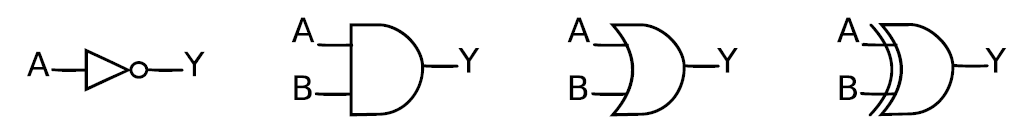
\includegraphics[scale=0.8]{immagini/gate}
	\caption{\textit{Gate elementari}}
	\label{fig1_1}
\end{figure} \\
La probabilità di '1' logico è stata stimata semplicemente andando a valutare il rapporto fra il numero di possibili combinazioni con '1' logico diviso il numero di combinazioni totali. Invece per il calcolo della Switching Activity è stata utilizzata la formula vista a lezione:
\begin{center}
	$ A=E_{SW}=P_{1}P_{0}+P_{1}P_{0}=2P_{1}(1-P_{1}) $
\end{center}
Dove $P_{1}$ e $P_{0}$ sono le probabilità di avere '1' e '0' logici in uscita dalla mia porta. \\
Di seguito si riportano i procedimenti matematici per ottenere le probabilità e le Switching Activity dei gate elementari visti in Figura \ref{fig1_1}.\\
\begin{itemize}
	\item \textit{Inverter} \\
	$P_{1}(Y)=P_{0}(A)=\frac{1}{2}$ \\
	$P_{0}(Y)=P_{1}(A)=\frac{1}{2}$ \\
	$E_{SW}=2P_{1}(Y)(1-P_{1}(Y))=2\frac{1}{2}\frac{1}{2}=\frac{1}{2}$\\
	\item \textit{AND} \\
	$P_{1}(Y)=P_{1}(A)P_{1}(B)=\frac{1}{2}\frac{1}{2}=\frac{1}{4}$ \\
	$E_{SW}=2P_{1}(Y)(1-P_{1}(Y))=2\frac{1}{4}\frac{3}{4}=\frac{3}{8}$\\
	\item \textit{OR} \\
	$P_{1}(Y)=P_{1}(A)P_{1}(B)+P_{0}(A)P_{1}(B)+P_{1}(A)P_{0}(B)=\frac{1}{2}\frac{1}{2}+\frac{1}{2}\frac{1}{2}+\frac{1}{2}\frac{1}{2}=\frac{3}{4}$ \\
	$E_{SW}=2P_{1}(Y)(1-P_{1}(Y))=2\frac{3}{4}\frac{1}{4}=\frac{3}{8}$\\
	\item \textit{XOR} \\
	$P_{1}(Y)=P_{1}(A)P_{0}(B)+P_{0}(A)P_{1}(B)=\frac{1}{2}\frac{1}{2}+\frac{1}{2}\frac{1}{2}=\frac{1}{2}$ \\
	$E_{SW}=2P_{1}(Y)(1-P_{1}(Y))=2\frac{1}{2}\frac{1}{2}=\frac{1}{2}$\\
\end{itemize}
Per maggiore chiarezza, i risultati sono raccolti nella Tabella \ref{Tab1_1}. \\
\begin{table}[!h]\footnotesize
	\centering
	\begin{tabular}{|c|c|c|c|c|}
		\hline
		 & \textbf{INVERTER}& \textbf{AND}& \textbf{OR} &\textbf{XOR}\\
		\hline
		$P_{1}(Y)$ & $1/2$  & $1/4$& $3/4$&$1/2$\\
		\hline
		$E_{SW}$& $1/2$ &$3/8$&$3/8$& $1/2$\\
		\hline
	\end{tabular}
	\caption{\textit{Risultati ottenuti manualmente}}
	\label{Tab1_1}
\end{table}\\
In seguito, tramite il programma \textit{ModelSim} è stato analizzato il numero di toogle delle varie porte utilizzando un testbench sviluppato appositamente dai docenti. Si è andato a variare il numero di colpi di clock, come richiesto dalla traccia ed in seguito si sono comparati i valori ottenuti dalla simulazione con ciò che si era calcolato manualmente.\\
Tramite appositi comandi di Modelsim (\textbf{-power report}), sono stati stilati dei report relativi ad una stima delle commutazioni delle varie porte, della quale se ne riporta un esempio in Figura \ref{fig1_2}. Questi report consentono di stimare l'attività delle porte come verrà descritto in seguito.\\
\begin{figure}[!htb]
	\centering
	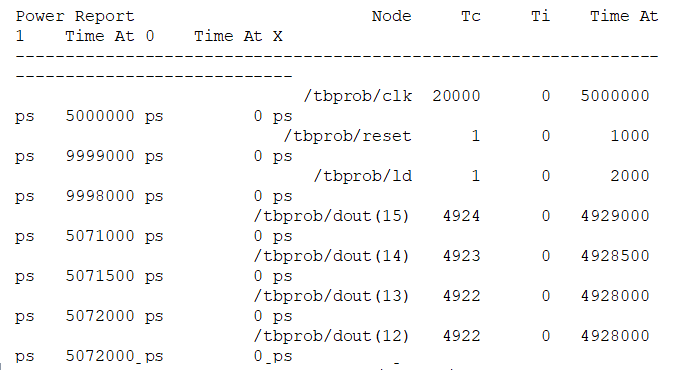
\includegraphics[scale=1]{immagini/fig1_2}
	\caption{\textit{Probabilità e Switching Activity stimati dal simulatore}}
	\label{fig1_2}
\end{figure} \\
Si riportano nella tabella \ref{tab1}, i risultati ottenuti dalle varie simulazioni.
\begin{table}[!h]\footnotesize
	\centering
	\begin{tabular}{|c|c|c|c|c|}
		\hline
		\textbf{Tc(CK)} & \textbf{Tc(INV)}& \textbf{Tc(AND)}& \textbf{Tc(OR)} &\textbf{Tc(XOR)}\\
		\hline
		20 & 1  & 5& 4&4\\
		\hline
		200 &  43 &40&42& 44\\
		\hline
		2000& 533& 418&352&470\\
		\hline
		20000& 4916& 3606&3784&4876\\
		\hline
	\end{tabular}
	\caption{\textit{Risultati simulazione}}
	\label{tab1}
\end{table}\\
Dai seguenti valori è facile ricavare i valori di Switching Activity simulate, in quanto si possono stimare da:
\begin{center}
	$ A=E_{SW}=\frac{Tc(PORT)}{T_{CLK}} $
\end{center}
Come ci si aspettava, essendo la Switching Activity il numero di toggle avvenuti in un periodo, i valori delle simulazioni vengono molto simili ai valori calcolati analiticamente. Aumentando il tempo di simulazione, i valori di Switching Activity diventano sempre più precisi, arrivando ad avere un errore tra 0.01-0.5. I vari valori sono stati calcolati e raccolti nella Tabella \ref{Tab1_2}
\begin{table}[!h]\footnotesize
	\centering
	\begin{tabular}{|c|c|c|c|c|}
		\hline
		\textbf{$N_{CLOCK}$} & \textbf{$E_{SW}(INV)$}& \textbf{$E_{SW}(AND)$}& \textbf{$E_{SW}(OR)$} &\textbf{$E_{SW}(XOR)$}\\
		\hline
		10 & 0.1  & 0.5& 0.4&0.4\\
		\hline
		100 &  0.43 &0.40&0.42& 0.44\\
		\hline
		1000& 0.533& 0.418&0.352&0.470\\
		\hline
		10000& 0.492& 0.36&0.378&0.487\\
		\hline
	\end{tabular}
	\caption{\textit{Switching activities calcolate}}
	\label{Tab1_2}
\end{table}\\

\section{Probability and Activity Calculation: Half and Full adder}
Nella seconda parte dell'esercitazione viene richiesto di analizzare le probabilità e la Switching Activity di un Half Adder e di un Full Adder, sia per quanto riguarda l'uscita $S$ sia per quanto riguarda il carry out $C_{OUT}$, dei quali se ne riporta lo schema circuitale rispettivamente in Figura \ref{half_adder} e \ref{full_adder}.
\begin{figure}[!htb]
	\centering
	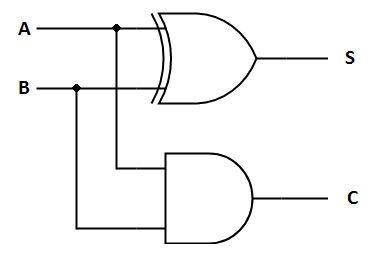
\includegraphics[scale=0.4]{immagini/half_adder}
	\caption{\textit{Schema circuitale Half Adder}}
	\label{half_adder}
\end{figure} \\
\begin{figure}[!htb]
	\centering
	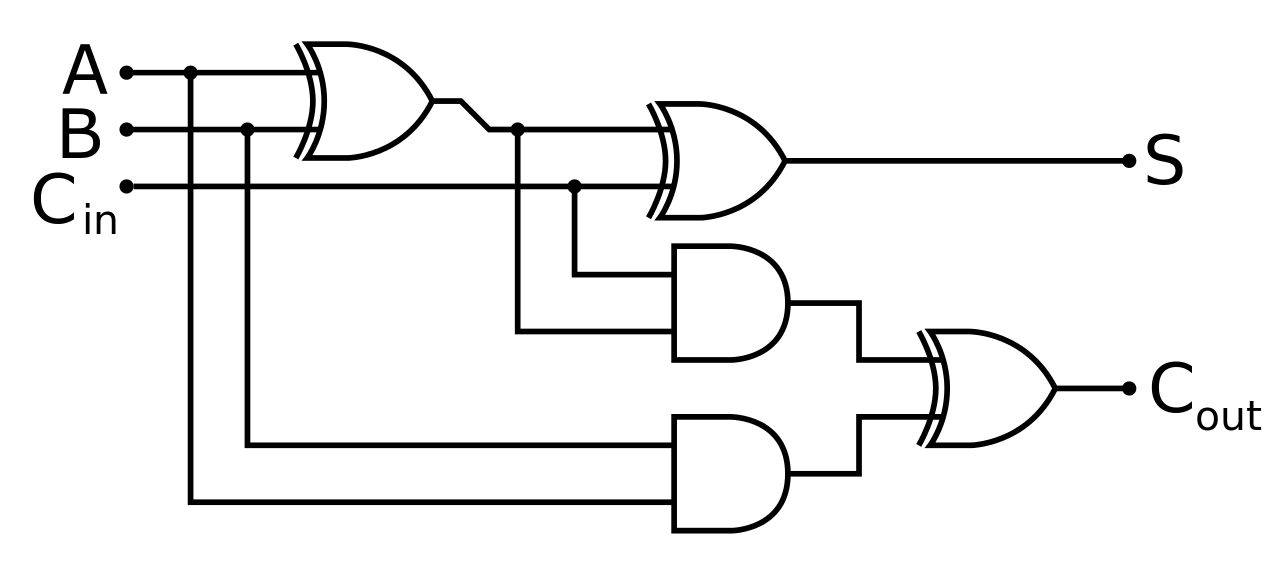
\includegraphics[scale=0.2]{immagini/full_adder}
	\caption{\textit{Schema circuitale Full Adder}}
	\label{full_adder}
\end{figure} \\
Il calcolo è stato effettuato in entrambi in casi, analizzando il blocco come un unico gate e andando a studiare la rispettiva Tavola di Verità. Anche in questa sezione, si considerano gli ingressi equiprobabili e scorrelati, con probabilità $P('input')=0.5$ Il risultato è stato il seguente:\\
\begin{itemize}
	\item \textit{Half-Adder} \\
	$P_{1}(S)=P_{1}(A)P_{0}(B)+P_{0}(A)P_{1}(B)=\frac{1}{2}\frac{1}{2}+\frac{1}{2}\frac{1}{2}=\frac{1}{2}$ \\
	$E_{SW}(S)=2P_{1}(S)(1-P_{1}(S))=2\frac{1}{2}\frac{1}{2}=\frac{1}{2}$\\
	$P_{1}(C_{OUT})=P_{1}(A)P_{1}(B)=\frac{1}{2}\frac{1}{2}=\frac{1}{4}$ \\
	$E_{SW}(C_{OUT})=2P_{1}(C_{OUT})(1-P_{1}(C_{OUT}))=2\frac{1}{4}\frac{3}{4}=\frac{3}{8}$\\
	\item \textit{Full-Adder} \\
	$P_{1}(S)=
	P_{0}(A)P_{0}(B)P_{1}(C_{IN})+
	P_{0}(A)P_{1}(B)P_{0}(C_{IN})+
	P_{1}(A)P_{0}(B)P_{0}(C_{IN})++
	P_{1}(A)P_{1}(B)P_{1}(C_{IN})
	=\frac{1}{2}\frac{1}{2}\frac{1}{2}+
	\frac{1}{2}\frac{1}{2}\frac{1}{2}+
	\frac{1}{2}\frac{1}{2}\frac{1}{2}+
	\frac{1}{2}\frac{1}{2}\frac{1}{2}=\frac{1}{2}$ \\
	$E_{SW}(S)=2P_{1}(S)(1-P_{1}(S))=2\frac{1}{2}\frac{1}{2}=\frac{1}{2}$\\
	$P_{1}(C_{OUT})=
	P_{0}(A)P_{1}(B)P_{1}(C_{IN})+
	P_{1}(A)P_{0}(B)P_{1}(C_{IN})+
	P_{1}(A)P_{1}(B)P_{0}(C_{IN})++
	P_{1}(A)P_{1}(B)P_{1}(C_{IN})+
	=\frac{1}{2}\frac{1}{2}\frac{1}{2}+
	\frac{1}{2}\frac{1}{2}\frac{1}{2}+
	\frac{1}{2}\frac{1}{2}\frac{1}{2}+
	\frac{1}{2}\frac{1}{2}\frac{1}{2}=\frac{1}{2}$ \\
	$E_{SW}(C_{OUT})=2P_{1}(C_{OUT})(1-P_{1}(C_{OUT}))=2\frac{1}{2}\frac{1}{2}=\frac{1}{2}$\\
\end{itemize}
I risultati sono sintetizzati nella Tabella \ref{Tab1_4}
\begin{table}[!h]\footnotesize
	\centering
	\begin{tabular}{|c|c|c|c|c|}
		\hline
		& $P(S=1)$&$P(C_{OUT}=1)$& $E_{SW}(S=1)$&$E_{SW}(C_{OUT}=1)$\\
		\hline
		\textbf{Half-Adder} & 1/2  & 1/4&1/2&3/8\\
		\hline
		\textbf{Full-Adder} &  1/2 &1/2&1/2& 1/2\\
		\hline
	\end{tabular}
	\caption{\textit{Risultati ottenuti manualmente}}
	\label{Tab1_4}
\end{table}\\

\noindent In seguito si sono calcolate, sempre analiticamente, le probabilità di uscita con le rispettive switching activities del Ripple Carry Adder, riportato in Figura \ref{ripple}, utilizzando i dati calcolati in precedenza per il singolo Full-Adder. Anche per questo calcolo iniziale gli ingressi sono stati considerati scorrelati ed equiprobabili.
\begin{figure}[!htb]
	\centering
	\includegraphics[scale=0.9]{immagini/ripple}
	\caption{\textit{Ripple Carry Adder}}
	\label{ripple}
\end{figure} \\
I risultati sono riportati nella Tabella \ref{Tab1_3}.\\
\begin{table}[!h]\footnotesize
	\centering
	\begin{tabular}{|c|c|c|c|c|c|c|c|c|}
		\hline
		&\textbf{FA7}& \textbf{FA6}& \textbf{FA5} &\textbf{FA4}&\textbf{FA3}&\textbf{FA2}&\textbf{FA1}&\textbf{FA0}\\
		\hline
		$P(S=1)$&1/2 &1/2&1/2&1/2&1/2&1/2&1/2&1/2\\
		\hline
		$E_{SW}$&1/2&1/2&1/2&1/2&1/2&1/2&1/2&1/2\\
		\hline
	\end{tabular}
	\caption{\textit{Probabilità e Switching Activity stimati manualmente con ingressi equiprobabili}}
	\label{Tab1_3}
\end{table}
\\
\noindent Se invece si considerano gli ingressi non equiprobabili, ma comunque scorrelati, con probabilità rispettivamente $P(A='1')=0.4$ e $P(B='1')=0.6 $, ci si aspetta un risultato differente, infatti le probabilità dei nodi di uscita trovate sono: $P(S ='1')=0.52$ e $P(Co ='1')=0.24$ \\
In seguito, tramite il programma \textit{ModelSim} è stato simulato il Ripple Carry Adder utilizzando un testbench sviluppato appositamente dai docenti e utilizzando le procedure viste nel paragrafo 1.1.\\
La simulazione viene fatta andando ad inserire dei ritardi sulle uscite $S$ e $C_{OUT}$ dei singoli Full-Adder. Inizialmente si setta esclusivamente un ritardo di 25 ps esclusivamente sul segnale $S$, mentre in secondo luogo si introduce un ritardo uguale anche sul segnale di $C_{OUT}$.\\
Il testbench è stato costruito appositamente per assegnare ritardi diversi al bit di somma, DRCAS, e al bit di carry, DRCAC. Inoltre per garantire una simulazione generale si è utilizzato l'LFSR per generare ingressi randomici. Per una corretta visualizzazione dei risultati si è impostata una risoluzione di 1ps. Dopo aver visualizzato il power report, come fatto già in precedenza, si sono comparati i valori ottenuti dalla simulazione con ciò che si era calcolato manualmente, seguendo lo stesso ragionamento del punto precedente.\\
	\begin{figure}[!htb]
		\centering
		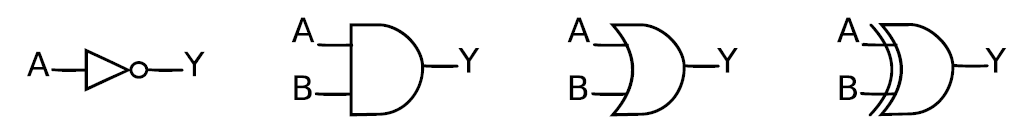
\includegraphics[scale=1]{immagini/gate}
		\caption{\textit{Power report}}
		\label{fig1_3}
	\end{figure} \\
	(cosa noto?) e bisogna mettere le waveforms?\\                                <- ATTENZIONE
Si è poi simulato il caso in cui i due ritardi riguardanti il bit di somma e il bit di carry fossero uguali, e anche per questo è stato visualizzato il power report.   
\begin{figure}[!htb]
		\centering
		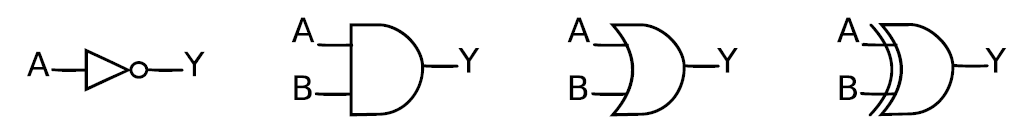
\includegraphics[scale=1]{immagini/gate}
		\caption{\textit{Power report con ritardi uguali}}
		\label{fig1_4}
	\end{figure} \\
	Da un analisi e confronto tra i risultati ottenuti manualmente e quelli ottenuti con le simulazioni, si nota come questi coincidano dato che avendo uguali ritardi, non riesco a simulare la presenza di eventuali glitch.\\
	In seguito si è calcolata la switching activity totale dei due sommatori, utilizzanso la seguente formula:
	\begin{center}
		$ A=\sum_{i=1}^{N-1}{A(S_i)} $  %<- risultato??
	\end{center}
What is the overhead computation of the second adder?  $<$- cioè? \\
Come ultima cosa è stato simulato il secondo testbench che ci è stato fornito, dove si simulava sempre un Ripple carry adder, ma questa volta in maniera puramente combinatoria.Analizzando i risultati, si può concludere come non avendo un segnale di temporizzazione, lavoro alla massima velocità ma ho la presenza di glitch.

\section{RCA synthesis and power analysis}
Nella seguente sezione dell'esercitazione è stata analizzata la potenza del sommatore RCA già analizzato in precedenza, tramite il software \textit{Synopsys}. Dopo aver analizzato ed elaborato i file che descrivono la struttura dell'RCA, il tutto è stato sintetizzato e sono stati raccolti i vari report relativi alla potenza.
Un primo report di potenza, riportato in Figura \ref{report_power1}, descrive i contributi di potenza relativi alle 8 istanze dei Full-Adder che compongono il somamtore RCA. \\
\begin{figure}[!htb]
	\centering
	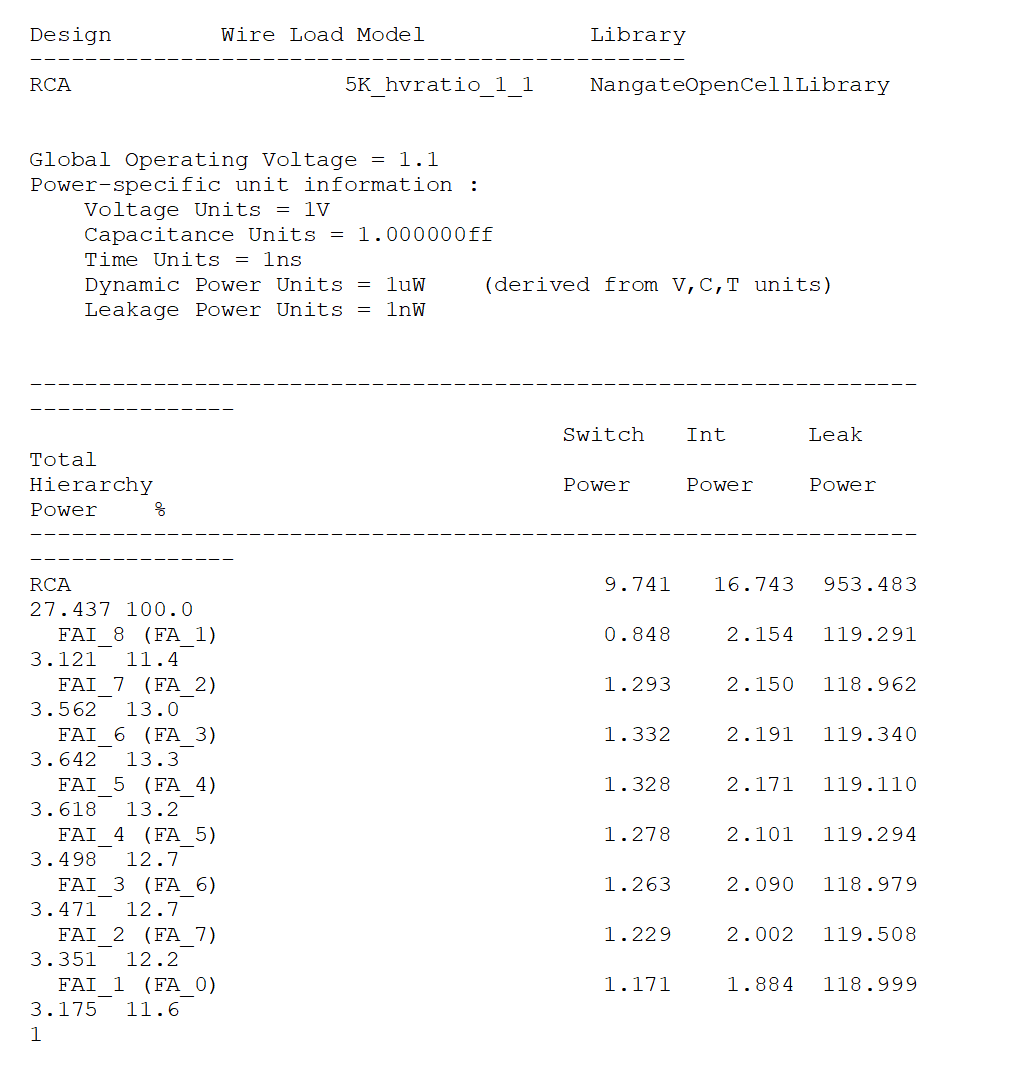
\includegraphics[scale=0.7]{immagini/report_power1}
	\caption{\textit{Power report}}
	\label{report_power1}
\end{figure}
\\
Come ci si aspettava, i contributi dei vari Full Adder sono tutti simili tra di loro, ad eccezione dell'istanza \textit{FAI\_8}: il motivo consiste nel fatto che il Carry Out dell'ultimo Full Adder non è connesso a nessun altra porta, dunque il carico da pilotare è decisamente minore.\\
Diventa ora interessante andare ad analizzare la singola istanza, per andare a valutare l'origine dei singoli contributi di potenza. Tramite il comando \textit{current\_instance FAI\_1} si va ad analizzare l'istanza relativa al primo Full Adder. Viene riportato il report in Figura \ref{reportFA1}.\\
\begin{figure}[!htb]
	\centering
	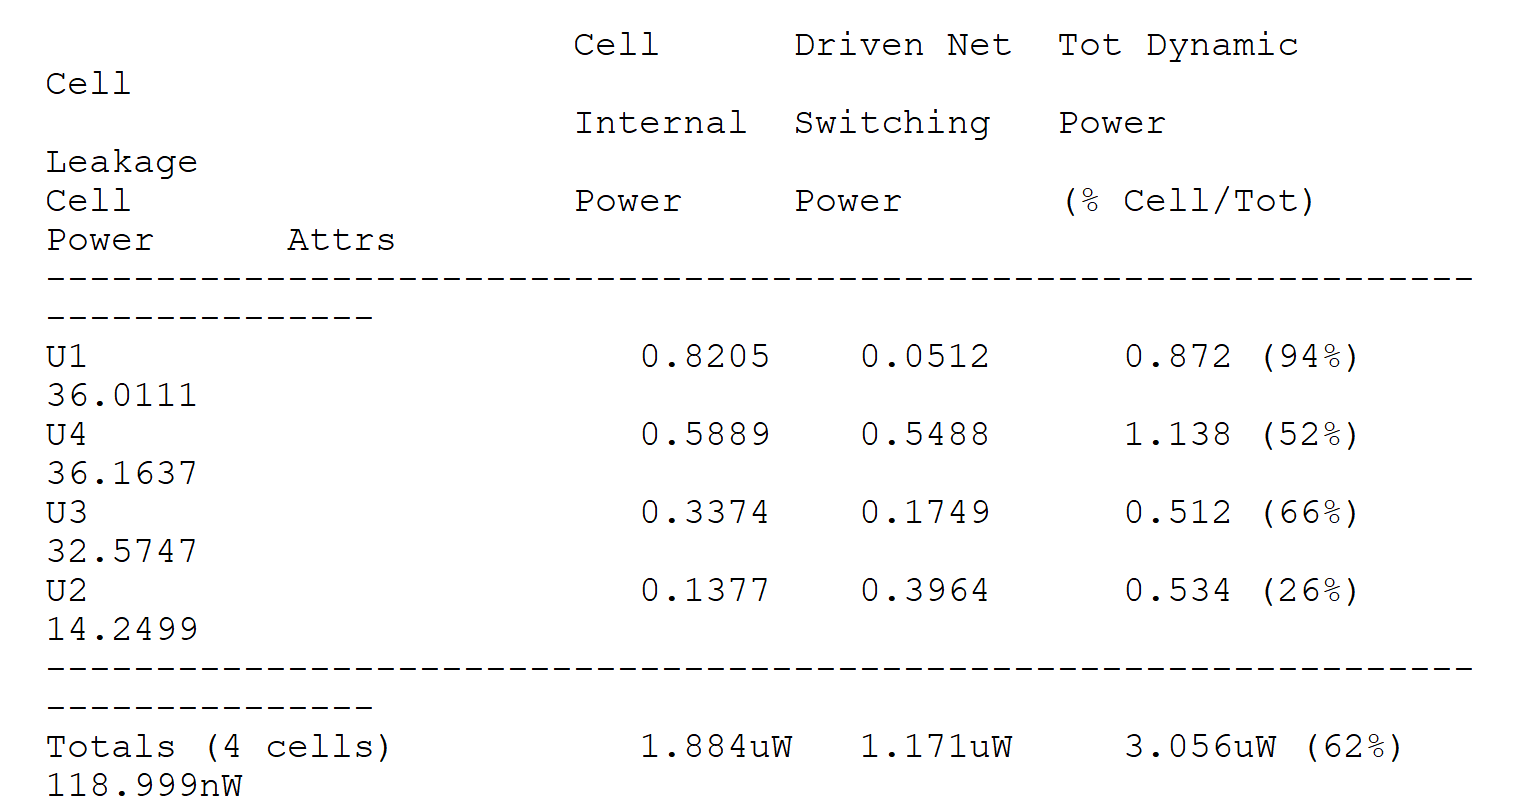
\includegraphics[scale=0.6]{immagini/reportFA1}
	\caption{\textit{Power report -current\_istance}}
	\label{reportFA1}
\end{figure}
\\
\\
\\
Come ci si aspettava i valori di potenza risultano assolutamente identici al report trovato in precendenza e riportato in Figura \ref{report_power1}.
Il passo successivo è comprendere come avvenga la stima della potenza dinamica (\textit{switching power}) dei singoli nodi del FA, dato che la potenza interna e quella di leakage dipendono solo dal gate e non dal circuito. Si utilizza a questo scopo il comando \textit{report\_power -net -verbose} e si riporta il report risultante in Figura \ref{verbose1}.
\begin{figure}[!htb]
	\centering
	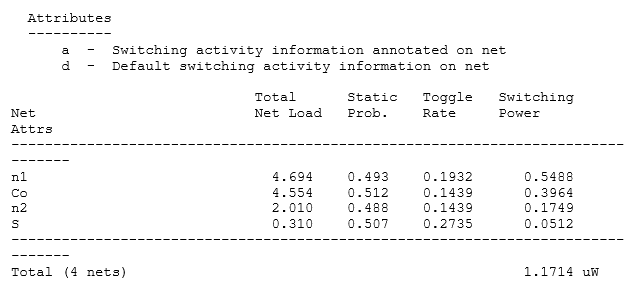
\includegraphics[scale=0.6]{immagini/verbose1}
	\caption{\textit{Power report -net -verbose}}
	\label{verbose1}
\end{figure}
\\
Si può notare come la potenza dinamica consumata dal nodo di uscita S sia praticamente nulla, in quanto essa non deve pilotare alcun carico, a meno della potenza che il software considera per le varie capacità parassite. \\
Con questa analisi, il software si preoccupa anche di fare un'analisi probabilistica delle varie attività dei nodi. Dal report si può notare come siano assolutamenti concordi con i valori teorici trovati in precedenza.\\
Si ritorna ora al circuito complessivo, salendo di livello logico e si analizzano i nodi anche in questa situazione utilizzando lo stesso comando utilizzato in precedenza. Il report viene raffigurato in Figura 1.11.
\begin{figure}[!htb]
	\centering
	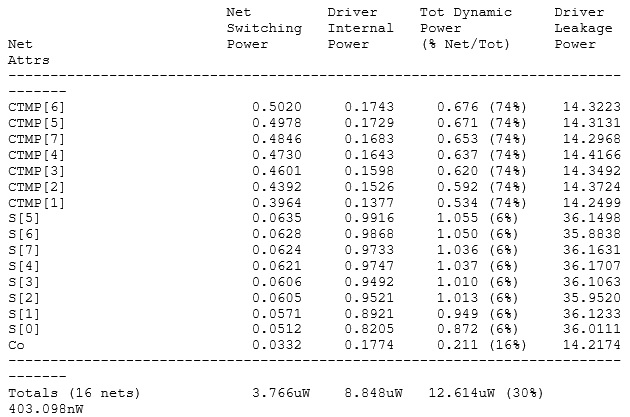
\includegraphics[scale=0.6]{immagini/verbose_2}
	\caption{\textit{Power report -net -verbose Full Adder}}
	\label{verbose_2}
\end{figure}

\section{A simple MUX: glitch generation and propagation}
\begin{figure}[!htb]
	\centering
	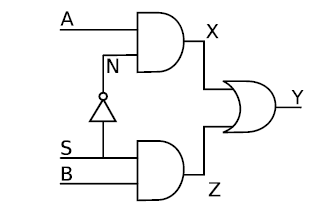
\includegraphics[scale=0.8]{immagini/mux}
	\caption{\textit{Mux}}
	\label{mux}
\end{figure}
\noindent Durante questa sezione, viene chiesto di analizzare il comportamento di un Multiplexer, riportato in Figura \ref{mux}, dove si assume che i ritardi delle varie porte elementari siano nulli, ad eccezione dell'Inverter che presenta un ritardo pari a 0,1 ns. Inizialmente si simula il circuito utilizzando \textit{ModelSim} e si riportano le one in Figura \ref{model_mux}.
\begin{figure}[!htb]
	\centering
	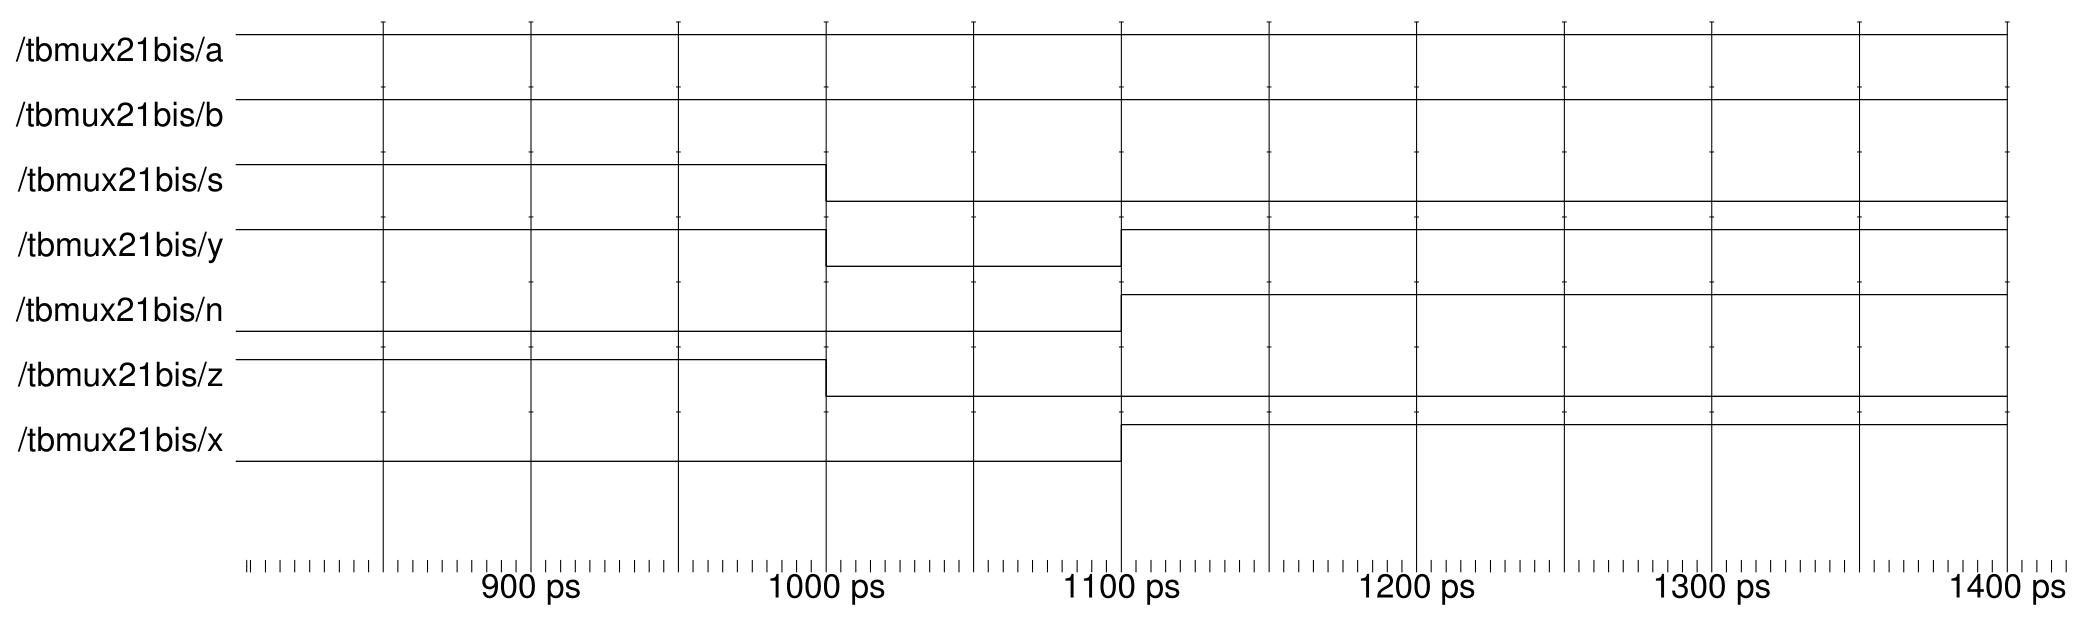
\includegraphics[scale=0.25]{immagini/model_mux}
	\caption{\textit{Mux's waves}}
	\label{model_mux}
\end{figure}
Si può notare benissimo come l'uscita Y abbia un glitch tra 1000 ps e 1100 ps, in quanto effettua una transizione 0-1 non voluta. Il tutto è causato dal ritardo introdotto dall'Inverter, che si può notare dal segnale 'n', che commuta al suo valore corretto dopo un ritardo di 0,1 ns, rispetto all'istante in cui cambiano tutti i restanti gate del circuito, ossia 1000 ps. Si verifica dunque un intervallo di tempo, ossia quello compreso tra 1000 ps e 1100 ps in cui la porta OR ha entrambi gli ingressi bassi e dunque produce un'uscita Y errata. \\
Questo produce quindi un glitch in uscita: in generale i glitch sono problematici a livello di potenza, in quanto si tratta di commutazioni spurie all'interno del mio circuito, che causano uno spreco di potenza. L'energia consumata per ogni doppia commutazione indesiderata è
\begin{center}
	$ E=C_{L}V_{DD}^{2}$
\end{center}
considerando $C_{L}$ come il carico che viene pilotato e $V_{DD}$ la tensione di alimentazione alla quale si lavora. 

\section{Probability and Activity Calculation: Syncronous Counter}
\begin{figure}[!htb]
	\centering
	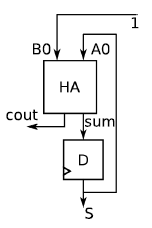
\includegraphics[scale=0.6]{immagini/counter}
	\caption{\textit{Counter 1 bit}}
	\label{counter}
\end{figure}
\noindent Si analizza in questa sezione un \textit{Syncronous Counter} ad 1 bit, realizzato con una Half Adder e un D-FlipFlop, riportato in Figura \ref{counter}. Il primo ingresso \textit{A0} dell'Half Adder è l'uscita del D-FlipFlop, mentre il secondo ingresso \textit{B0} viene collegato fisso ad 1. Si riporta il timing diagram del circuito in Figura \ref{timing_counter1}.
%%MANCA TIMING DA FARE
Si può dedurre dal timing, che il segnale \textit{S} ha una transizione per ogni colpo di clock, di conseguenza la sua Switching Activity sarà metà dell'attività del segnale di clock. Nel caso in cui il segnale B0 vada a 0, il valore del nodo S dipenderà esclusivamente dall'ultimo valore presente all'uscita del Flip-Flop, in quanto l'Half Adder sommerà l'ultimo valore presente nel Flip Flop con uno '0'. Quindi non si verificheranno più transizioni sul nodo S e di conseguenza neanche sul nodo $C_{OUT}$.
\begin{figure}[!htb]
	\centering
	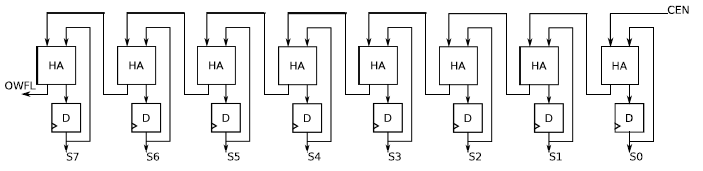
\includegraphics[scale=0.6]{immagini/counter2}
	\caption{\textit{Counter 8 bit}}
	\label{counter2}
\end{figure}
In seguito viene chiesto di analizzare la struttura presente in Figura \ref{counter2}. Questo circuito permette di ottenere un contatore sincrono ad 8 bit, utilizzando in cascata 8 celle del circuito precedente. Anche in questo si riporta, in Figura \ref{timing_counter2}, il timing diagram del funzionamento del circuito.
%MANCA TIMING
In Tabella \ref{trans_uscita}, vengono ora riportati il numero di commutazioni di tutti i segnali di uscita ricavati in modo analitico, considerando un intervallo di tempo compreso da quando il circuito parte dal valore '00000000', fino a quando non arriva al valore '11111111'.
\begin{table}[!h]\footnotesize
	\centering
	\begin{tabular}{|c|c|}
		\hline
		\textbf{Signal} & \textbf{Number of Transitions}\\
		\hline
		Clock & 511  \\
		S0 &  255 \\
		S1&127\\
		S2& 63\\
		S3& 31\\
		S4& 15\\
		S5& 7\\
		S6& 3\\
		S7& 1\\
		\hline
	\end{tabular}
	\caption{\textit{Risultati simulazione}}
	\label{trans_uscita}
\end{table}\\

Il segnale \textit{CEN}, rappresenta l'enable del contatore, mentre il segnale \textit{OWFL} va ad 1 in presenza di overflow, dunque quando si supera la massima dinamica del contatore. Il segnale CEN è l'ingresso B0 del primo Half-Adder, mentre il segnale OWFL è il carry out dell'ultimo Half-Adder. \\
Il Segnale OWFL farà solo una transizione per ogni ciclo di conta, dunque andrà ad '1', solo quando le uscite S7-S0 andranno dal valore '11111111' al valore '00000000'. Di conseguenza avrò che la Switching Activity sarà:
\begin{center}
	$E_{SW}=\frac{1}{2^{8}-1}=$
\end{center}
Si vuole ora confrontare i risultati analitici ricavati in precedenza ed i risultati ottenuti sfruttando le simulazione di \textit{Synopsis}. In Figura \ref{report_counter}, viene riportata la simulazione ottenuta.\\
\begin{figure}[!htb]
	\centering
	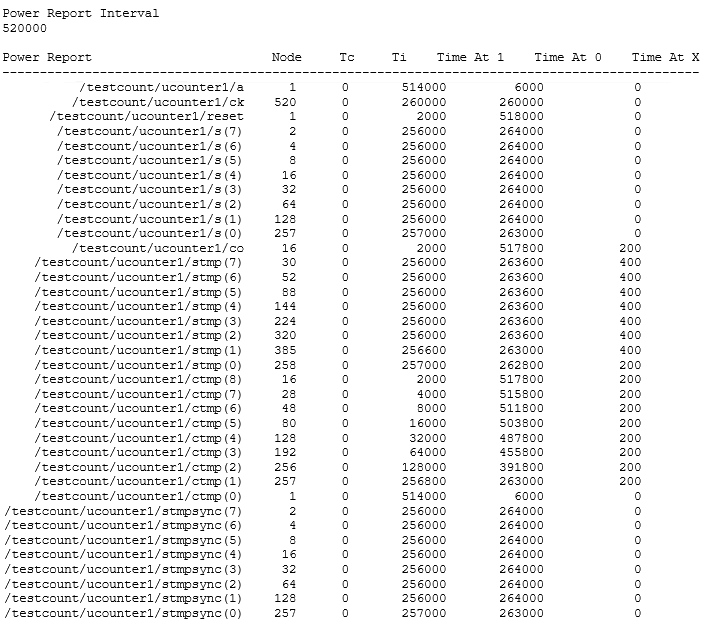
\includegraphics[scale=0.6]{immagini/report_counter}
	\caption{\textit{Power report}}
	\label{report_counter}
\end{figure}
Viene chiesto di confrontare i valori analitici calcolati e riportati nella Tabella \ref{trans_uscita}, con quelli derivanti da una simulazione \textit{Synopsis}. Si simula il comportamento del circuito utilizzando un $T_{CLK}=2 ns$, per un periodo pari a 260 colpi di clock. Il report risultante è presente in Figura \ref{report_counter}.
Andando a studiare i file di testbench riportati, si può notare come vengano introdotti dei ritardi di 0.2 ns nelle uscite dell'Half Adder: questo provoca dei glitch che si andranno a propagare lungo la rete ed avranno effetti sul segnale OWFL, che invece di andare ad '1' solo una volta a fine conteggio, andrà ad '1' per tre volte (DA VERIFICARE!!!).\\
Tramite il power report si può notare come, in generale, il numero di commutazioni della simulazione sia superiore a quello ottenuto analiticamente: si può notare questo fenomeno nei segnali \textit{stmp(n)}, ossia le uscite non sincrone dei Flip Flop, e nei segnali di Carry Out. Il tutto è dovuto ai glitch che si propagano interamente al contatore a causa del ritardo di 0.2 ns di ciascun Half Adder. \\
Fortunatamente, questi glitch vengono filtrati dai Flip-FLop, in quanto il $T_{CLK}$ è superiore al ritardo introdotto dalla rete combinatoria.

	\chapter{Laboratorio 2: \\FSM State Assignment and VHDL Synthesis}
\section{FSM State Assignment}
Durante la prima parte dell'esercitazione di laboratorio, viene richiesto di implementare un circuito per sommare 6 numeri
\begin{center}
	$s=a+b+c+d+e+f $
\end{center}
utilizzando un unico sommatore, due multiplexer e un registro. Viene richiesto di valutare e minimizzare il consumo di potenza, andando a modificare la connessione degli input A-H, considerando esclusivamente l'attività della FSM e i bit di selezione del MUX S0-S3.\\
Il circuito completo è riportato in Figura \ref{datapath}, mentre la FSM è presente in Figura \ref{fsm}.\\
\begin{figure}[!htb]
	\centering
	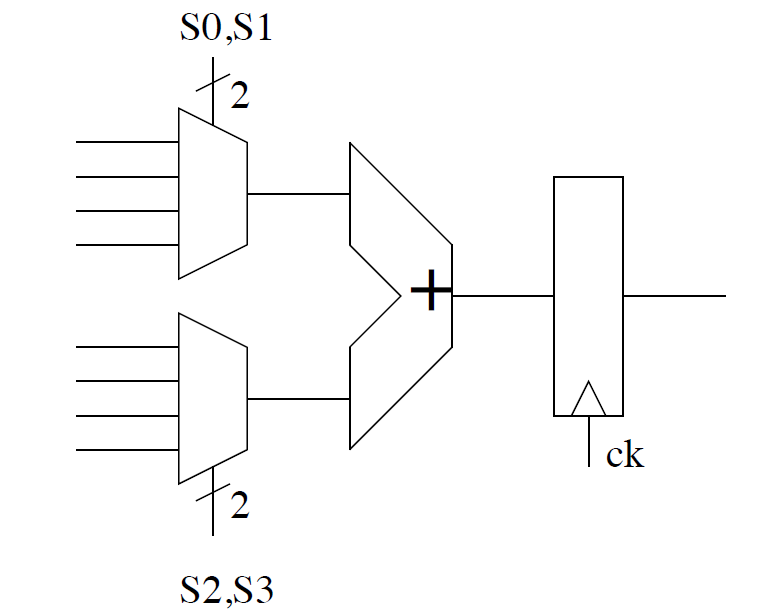
\includegraphics[scale=0.6]{immagini/circuito}
	\caption{\textit{Probabilità e Switching Activity stimati manualmente}}
	\label{datapath}
\end{figure} \\
Dopo varie ottimizzazioni, si è arrivati ad avere un'attività totale pari a 8 per il multiplexer e 6 per la State transition della macchina a stati, andando a considerare che la macchina a stati e il multiplexer ricomincino le operazioni una volta terminate. Nella tabella \ref{tab2} viene riportata la configurazione degli stati e dei bit del multiplexer scelta:
\begin{table}[!h]\footnotesize
	\centering
	\begin{tabular}{|c|c|}
		\hline
		\textbf{STATI} & \textbf{$S_{3}S_{2}S_{1}S_{0}$}\\
		\hline
		000 & 0000\\
		\hline
		001 &0101 \\
		\hline
		011& 0111\\
		\hline
		010& 1110\\
		\hline
		110& 1010\\
		\hline 
	\end{tabular}
	\caption{\textit{Risultati simulazione}}
	\label{tab2}
\end{table} \\


\section{VHDL synthesis}
Il secondo punto del laboratorio prevede di sintetizzare l’FSM tramite synopsys e studiarne le caratteristiche in termini di area, potenza e timing in modo da ricercare possibili ottimizzazioni.\\
Si è utilizzata la libreria a 45 nm, definito un segnale di clock di periodo corrispondente a 10 ns, si è verificato il corretto inserimento tramite il comando \emph{report_clock} e si è sintetizzato il circuito.\\

	\chapter{Laboratorio 3: \\Clock gating, pipelining and parallelizing}
Durante questa esperienza di laboratorio verranno analizzate una serie di tecniche per ridurre i consumi mediante l'ottimizzazione dell'architettura dei circuiti.
\section{A first approach to clock gating}
Un prima tecnica utilizzata per ridurre i consumi andando a lavorare sull'architettura è il \textit{Clock Gating}. Questa tecnica permette di "staccare" il clock ad un determinato blocco del mio circuito, quando questo non deve lavorare. Un circuito di massima è riportato in Figura \ref{clock_gating}. \\
\begin{figure}[!htb]
	\centering
	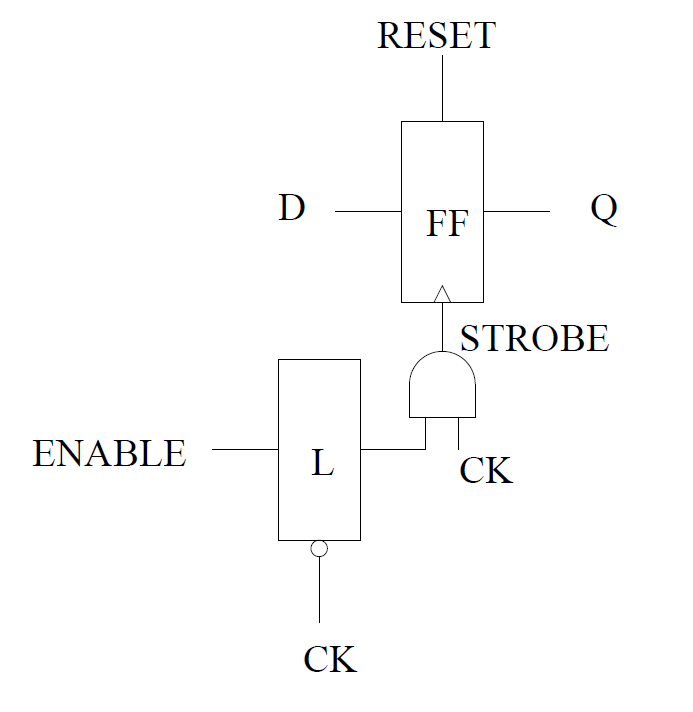
\includegraphics[scale=0.60]{immagini/clock_gating}
	\caption{\textit{Schema implementativo della tecnica del Clock Gating}}
	\label{clock_gating}
\end{figure}
\newpage
\noindent Nella prima parte dell'esperienza viene chiesto di analizzare il file \textit{ckgbug.vhd} che contiene la descrizione VHDL di una struttura composta da due registri in cascata, denominati L1 ed L2. La tecnica del clock gating viene applicata al secondo registro, mediante una AND tra il clock e un segnale di ENABLE. \\
Bisogna prestare attenzione al fatto che i segnali di ingresso dei due registri (D1 e D2) siano rispettivamente \textit{std\_logic\_vector (7 downto 0)} e \textit{std\_logic\_vector (0 to 7)}. \\
In una prima simulazione, si forza il segnale D1 al valore '01111111' e, attivando il segnale di ENABLE, ci si aspetterebbe che D2, al colpo di clock successivo, vada al valore '111111110' e che l'uscita di L2, denominata D3, vada al valore '01111111' al colpo di clock ancora successivo. In realtà la simulazione porta al risultato in Figura \ref{clock_gat1}.
\begin{figure}[!htb]
	\centering
	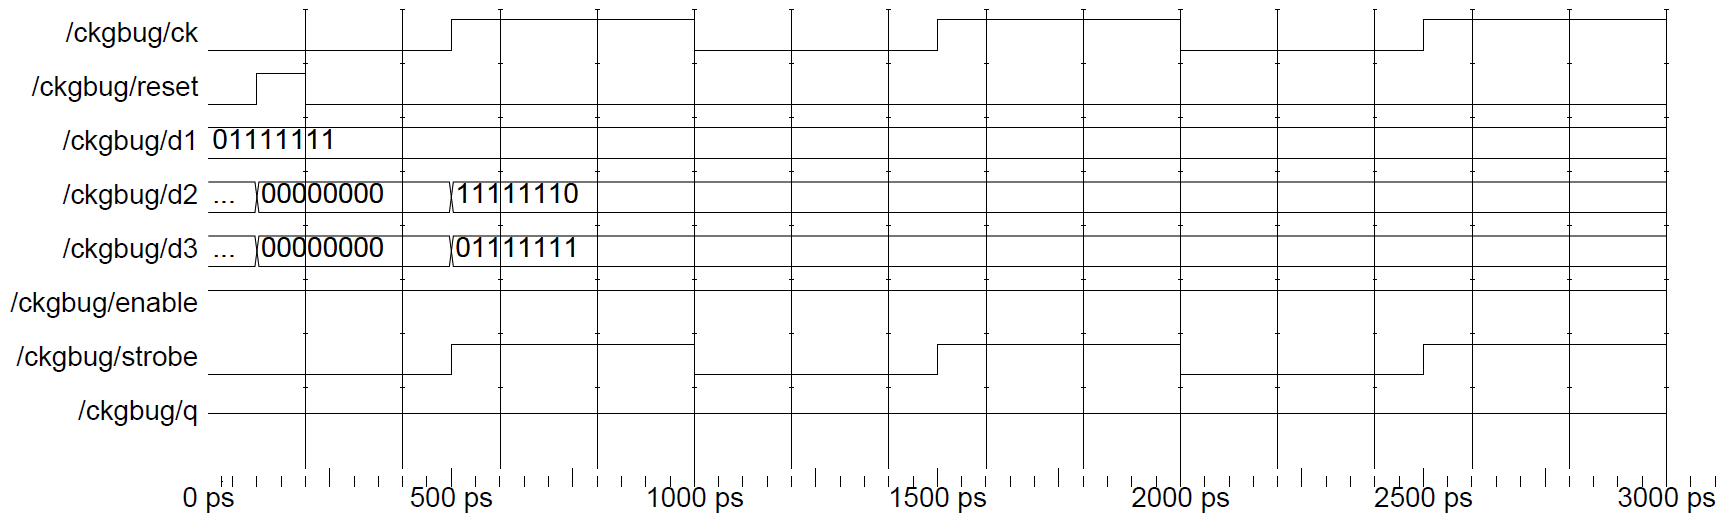
\includegraphics[scale=0.6]{immagini/clock_gating1}
	\caption{\textit{Timing simulazione}}
	\label{clock_gat1}
\end{figure}
Si può ben notare come l'uscita D3 dopi esattamente D1 dopo un solo colpo di clock. Questo è dovuto al fatto che il clock gated arriva a L2 un "passo di simulazione" dopo L1, perchè il simulatore programma il calcolo dell'uscita AND dopo l'assegnazione del clock. Quindi accade come se l'AND avesse un ritardo interno. \\
La traccia suggerisce che si può risolvere questo inconveniente andando ad aggiungere un ritardo \textit{Clock-to-Output} pari a 0.1 ps all'uscita del generico Flip-Flop. Andando a risimulare il file, si ottiene il comportamento desiderato, che viene riportato in Figura \ref{clock_gat2}. \\
\newpage
\begin{figure}[!htb]
	\centering
	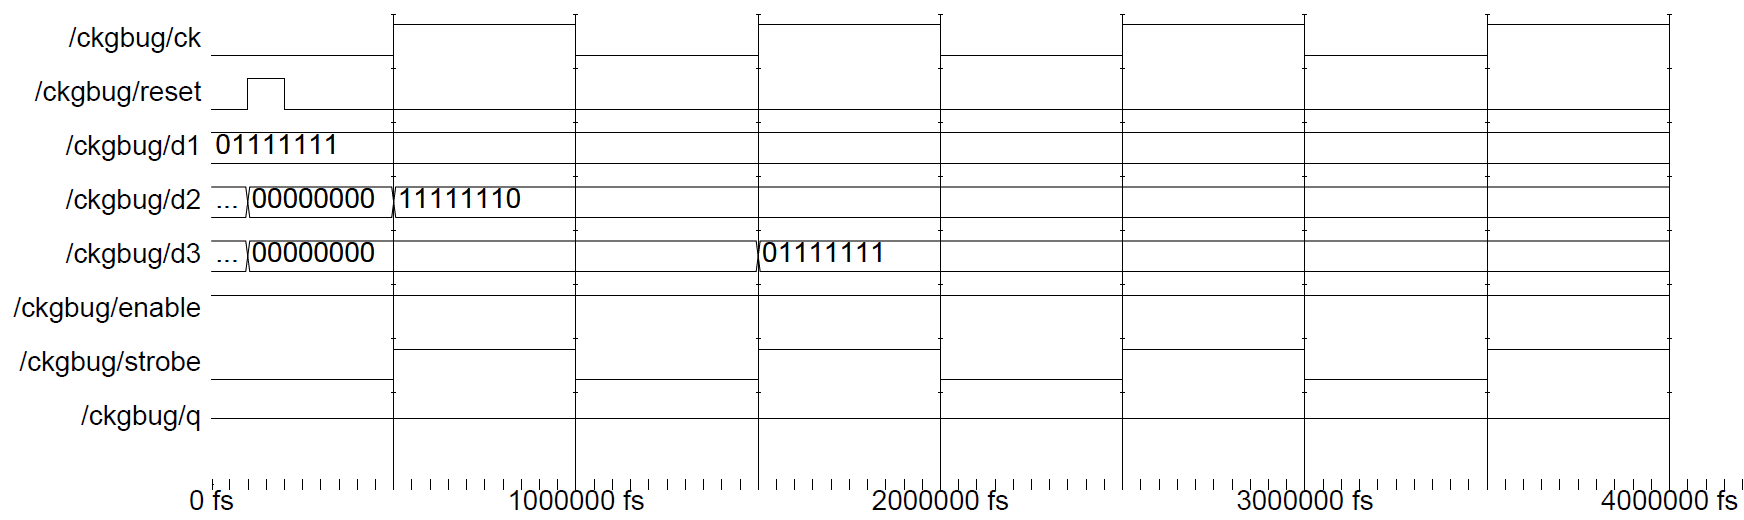
\includegraphics[scale=0.6]{immagini/clock_gating2}
	\caption{\textit{Timing simulazione con ritardo clk-to-out=0.1ps}}
	\label{clock_gat2}
\end{figure}
\noindent Infine si aggiunge un ulteriore ritardo alla porta AND pari a 0.2 ps, ossia un tempo superiore a quello \textit{Clock-to-Output} inserito in precendenza. In questo modo si va a violare il $t_{hold}$ e dunque il circuito ritorna nella situazione precedente con un funzionamento non corretto. Il risultato della simulazione è riportato in Figura \ref{clock_gat3}. \\
\begin{figure}[!htb]
	\centering
	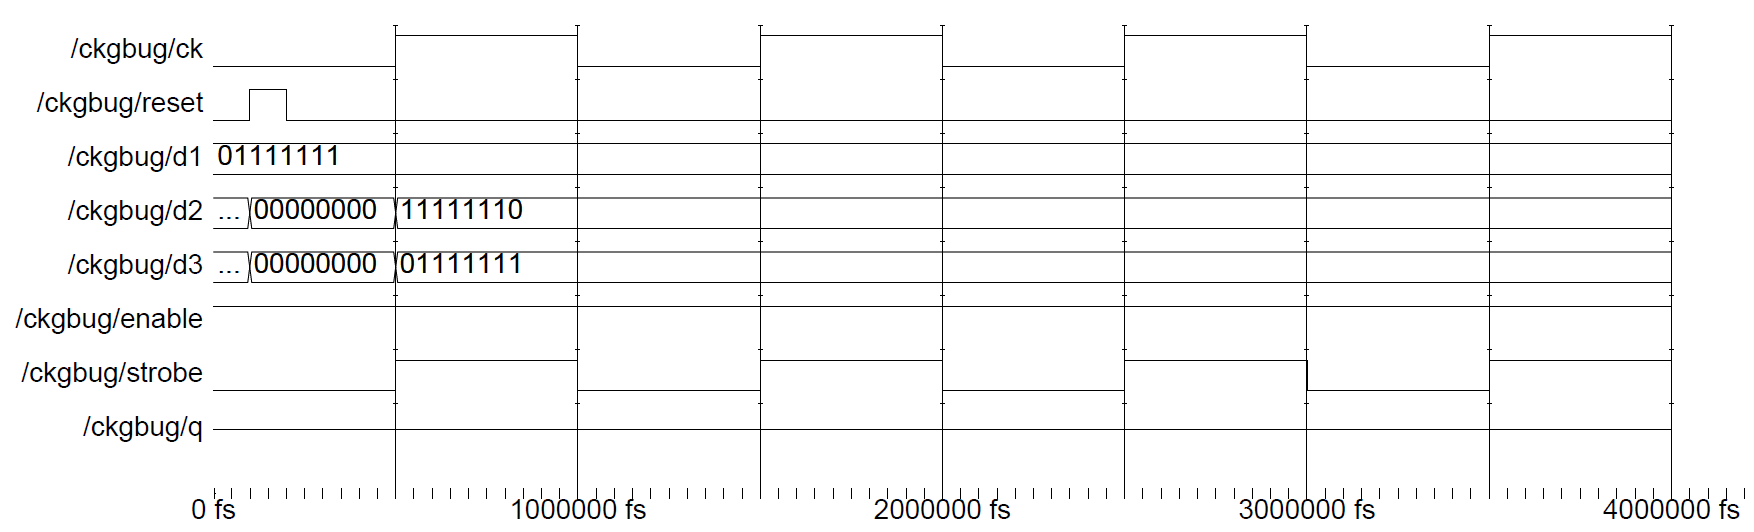
\includegraphics[scale=0.6]{immagini/clock_gating3}
	\caption{\textit{Timing simulazione, ritardo AND di 0.2ps}}
	\label{clock_gat3}
\end{figure}
\newpage
\section{Clock Gating for a complex circuit}
Nella seguente sezione viene chiesto di analizzare il funzionamento e in seguito il consumo di potenza, applicando il concetto del clock gating, nel circuito illustrato in Figura \ref{circuito_3_2}.\\
\begin{figure}[!htb]
	\centering
	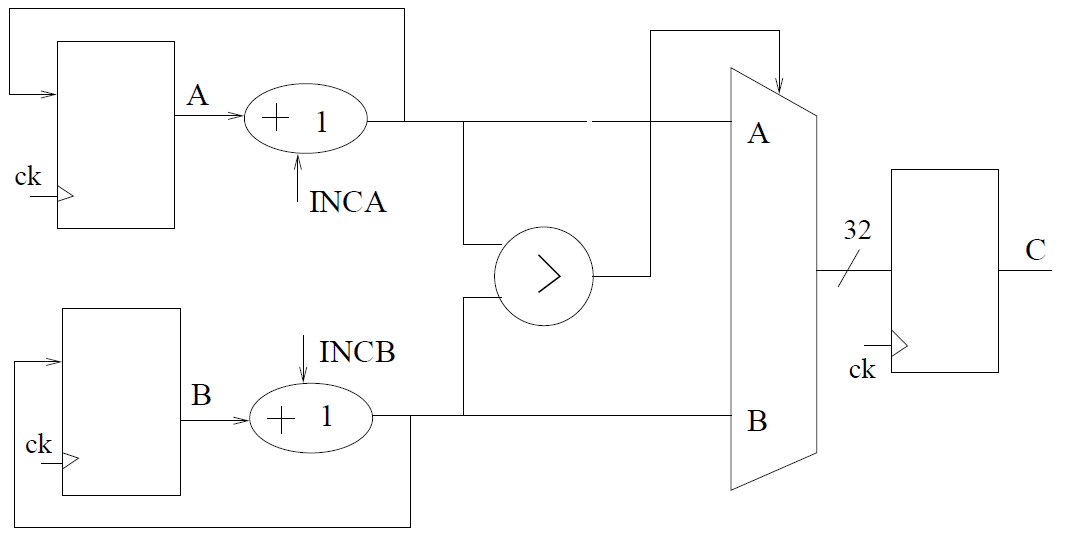
\includegraphics[scale=0.8]{immagini/circuito_3_2}
	\caption{\textit{Schema circuito}}
	\label{circuito_3_2}
\end{figure}
\\
Si prova, esclusivamente a livello cartaceo ad applicare la tecnica del Clock Gating al circuito in figura, ottenendo il circuito in Figura \ref{clkgating}.\\
\begin{figure}[!htb]
	\centering
	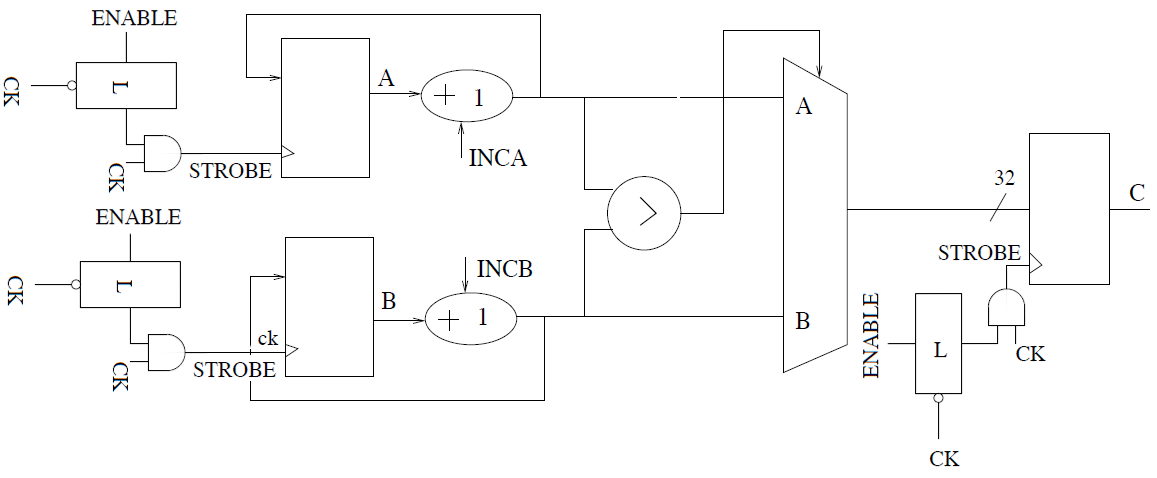
\includegraphics[scale=0.3]{immagini/clkgating}
	\caption{\textit{Schema circuito con clock gating}}
	\label{clkgating}
\end{figure}
\\
Si è proceduto dunque alla sintesi del circuito, sempre tramite \textit{Synopsis}, creando un clock con periodo pari a 5 s. Tramite il comando \textit{report\_power -include\_input\_nets} si è potuto ricavare un resoconto dei contributi di potenza dissipata, che vengono riportati in Figura \ref{3_1}. \\
\begin{figure}[!htb]
	\centering
	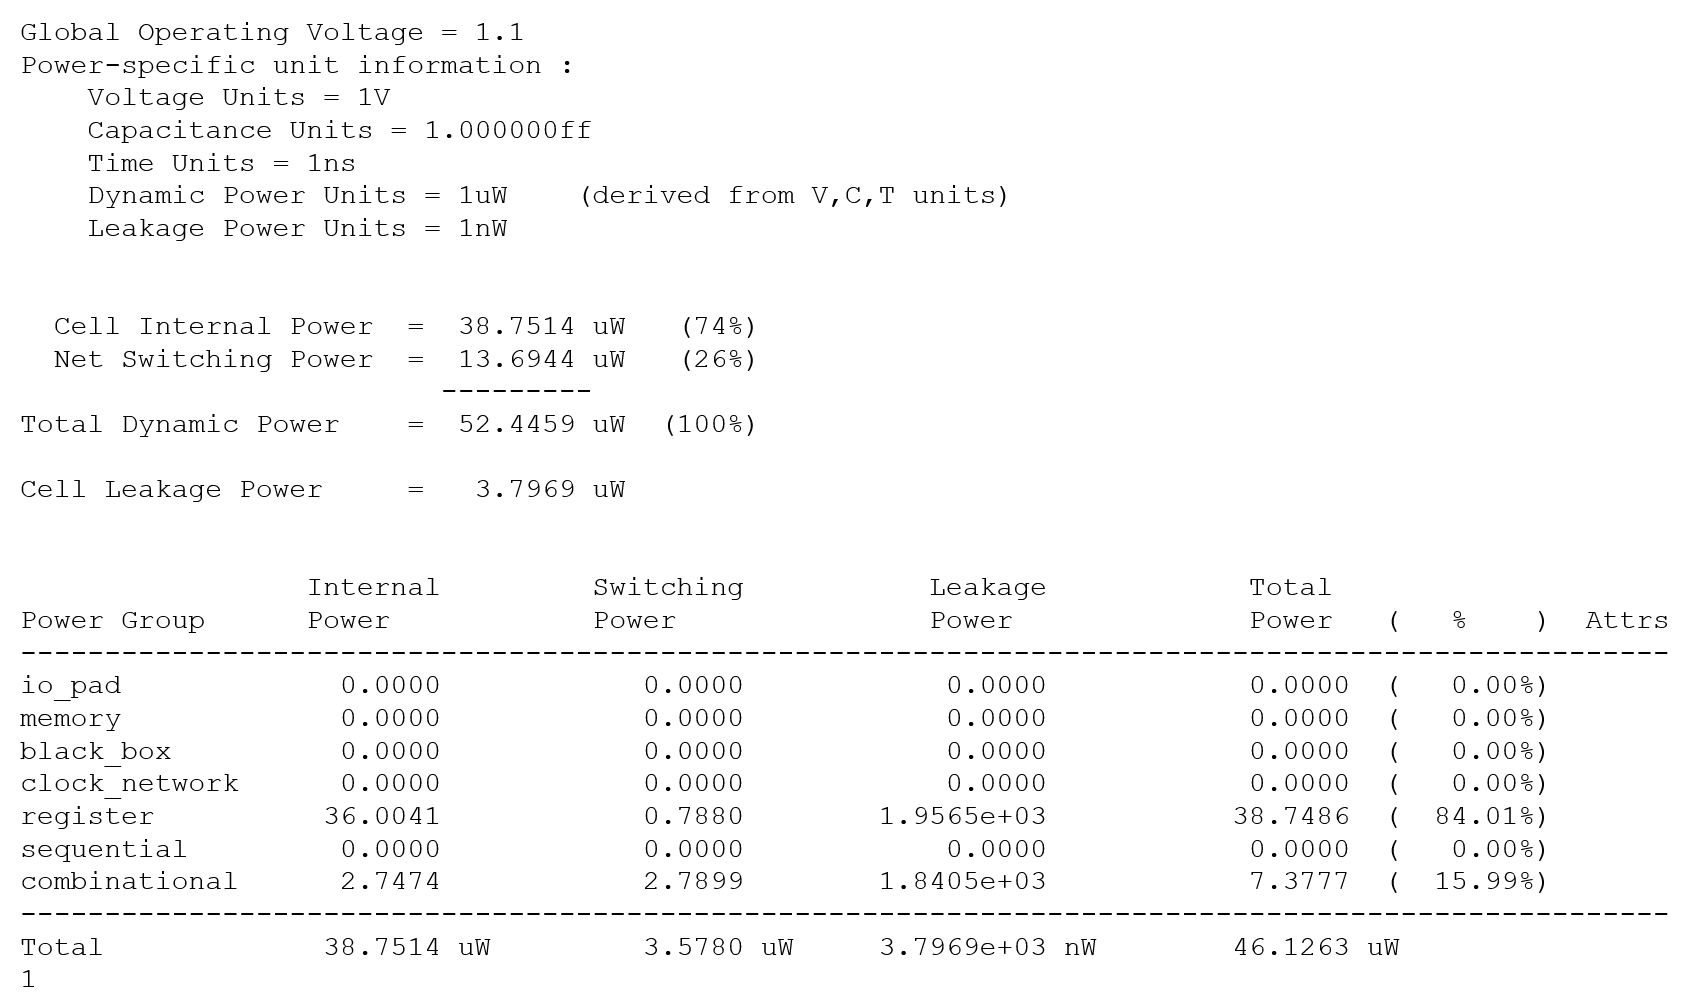
\includegraphics[scale=0.8]{immagini/3_1}
	\caption{\textit{Power report nets}}
	\label{3_1}
\end{figure}
\\
Si è poi andato ad eseguire un'analisi più dettagliata dei contributi tramite il comando \textit{report\_power -net -include\_input\_nets}, che viene riportato in Figura \ref{3_2}. \\
\begin{figure}[!htb]
	\centering
	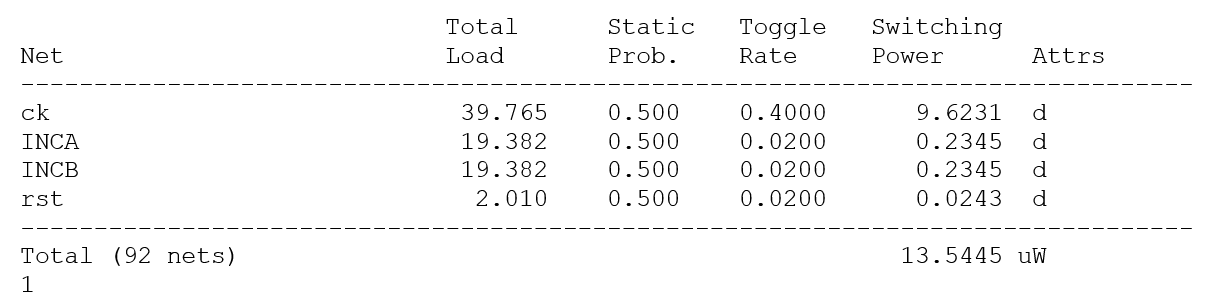
\includegraphics[scale=0.8]{immagini/3_2}
	\caption{\textit{Power report input nets}}
	\label{3_2}
\end{figure}
\\
Come si può ben notare dalla quarta colonna, il toogle rate dei vari ingressi presenta una \textit{static probability} pari a 0.5, che non risulta essere un valore sempre ragionevole. \\
Questo valore viene assegnato di default dal software, che però, tramite degli appositi comandi, permette di settare valori diversi di Toogle Rate a determinati segnali. Si è allora modificato il toggle rate del clock e del reset portandoli rispettivamente a 2 e a 0. Queste modifiche portano ad un risparmio di potenza del 20\% rispetto al caso precedente. Il report di potenza risultante viene raffigurato in Figura \ref{3_3}.
\begin{figure}[!htb]
	\centering
	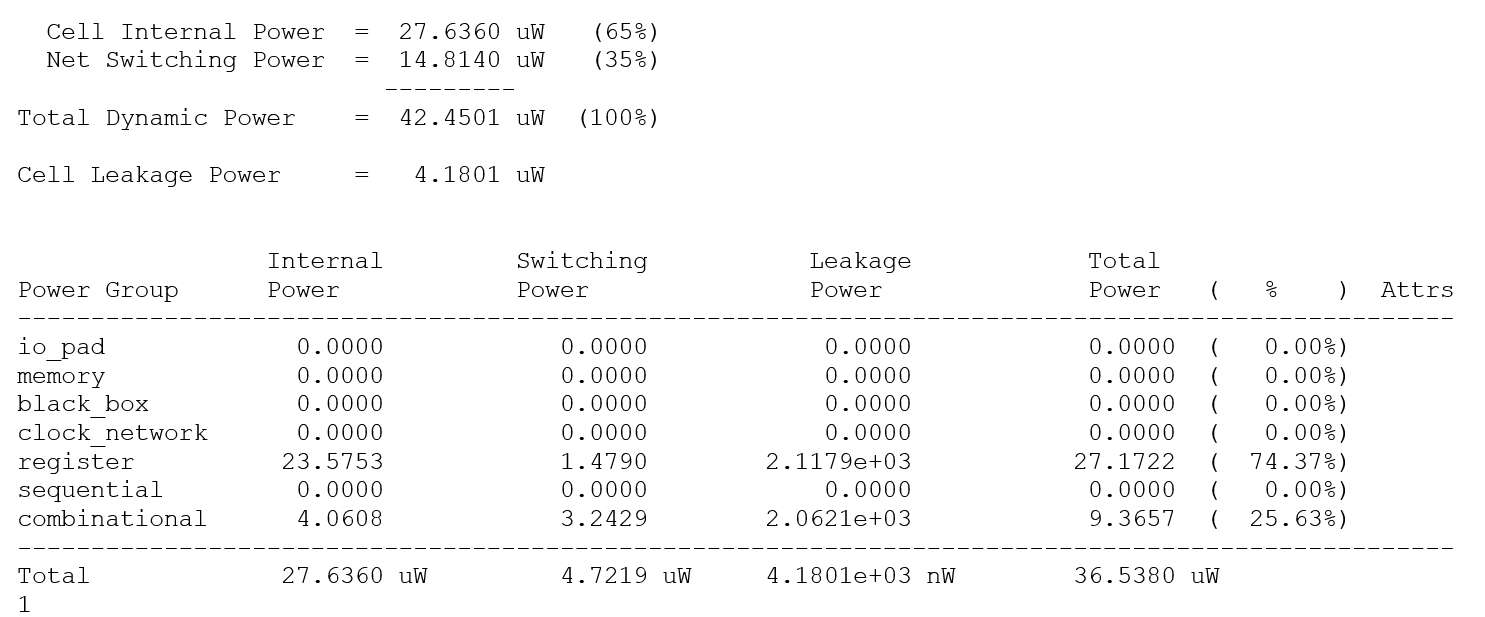
\includegraphics[scale=0.8]{immagini/3_3}
	\caption{\textit{Power report con toggle del clock pari a 2}}
	\label{3_3}
\end{figure}
Si va ora a modificare anche la probabilità degli input, portando sia INCA che INCB ad un Toogle Rate pari a 0.12. Si ottiene allora un risparmio ulteriore di potenza, come testimoniato da Power Report riportati in Figura \ref{3_4} e \ref{3_5}.
\begin{figure}[!htb]
	\centering
	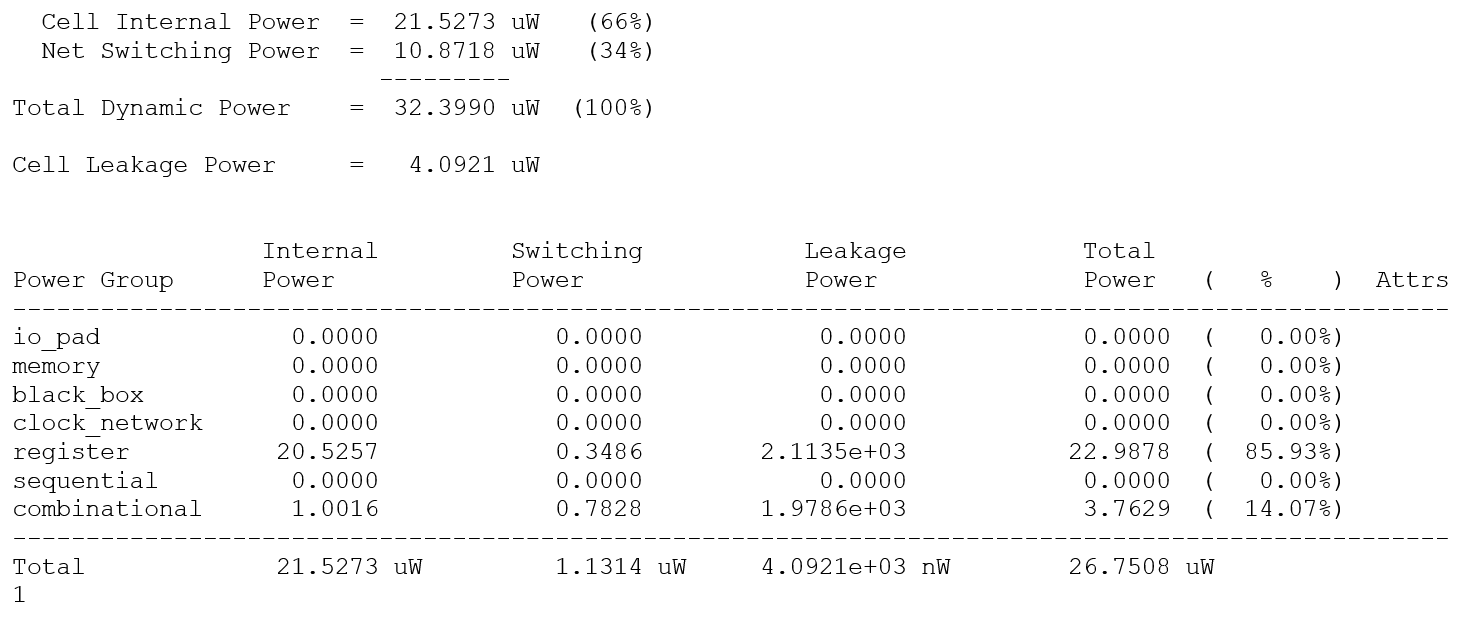
\includegraphics[scale=0.8]{immagini/3_4}
	\caption{\textit{Schema implementativo della tecnica del Clock Gating}}
	\label{3_4}
\end{figure}
\begin{figure}[!htb]
	\centering
	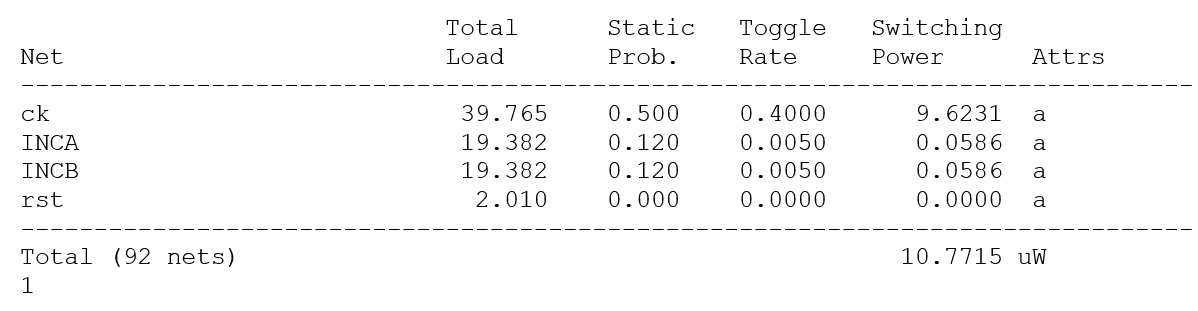
\includegraphics[scale=0.8]{immagini/3_5}
	\caption{\textit{Schema implementativo della tecnica del Clock Gating}}
	\label{3_5}
\end{figure}
\newpage
\noindent Infine, tramite il comando \textit{report cell}, si riesce ad ottenere il numero di celle impiegate con la relativa dimensione. Viene riportato in Figura \ref{3_6}. Si può ben notare come nel caso analizzato le celle siano 74 e l'area utilizzata sia $229.292007 \mu m^{2}$ \\
\begin{figure}[!htb]
	\centering
	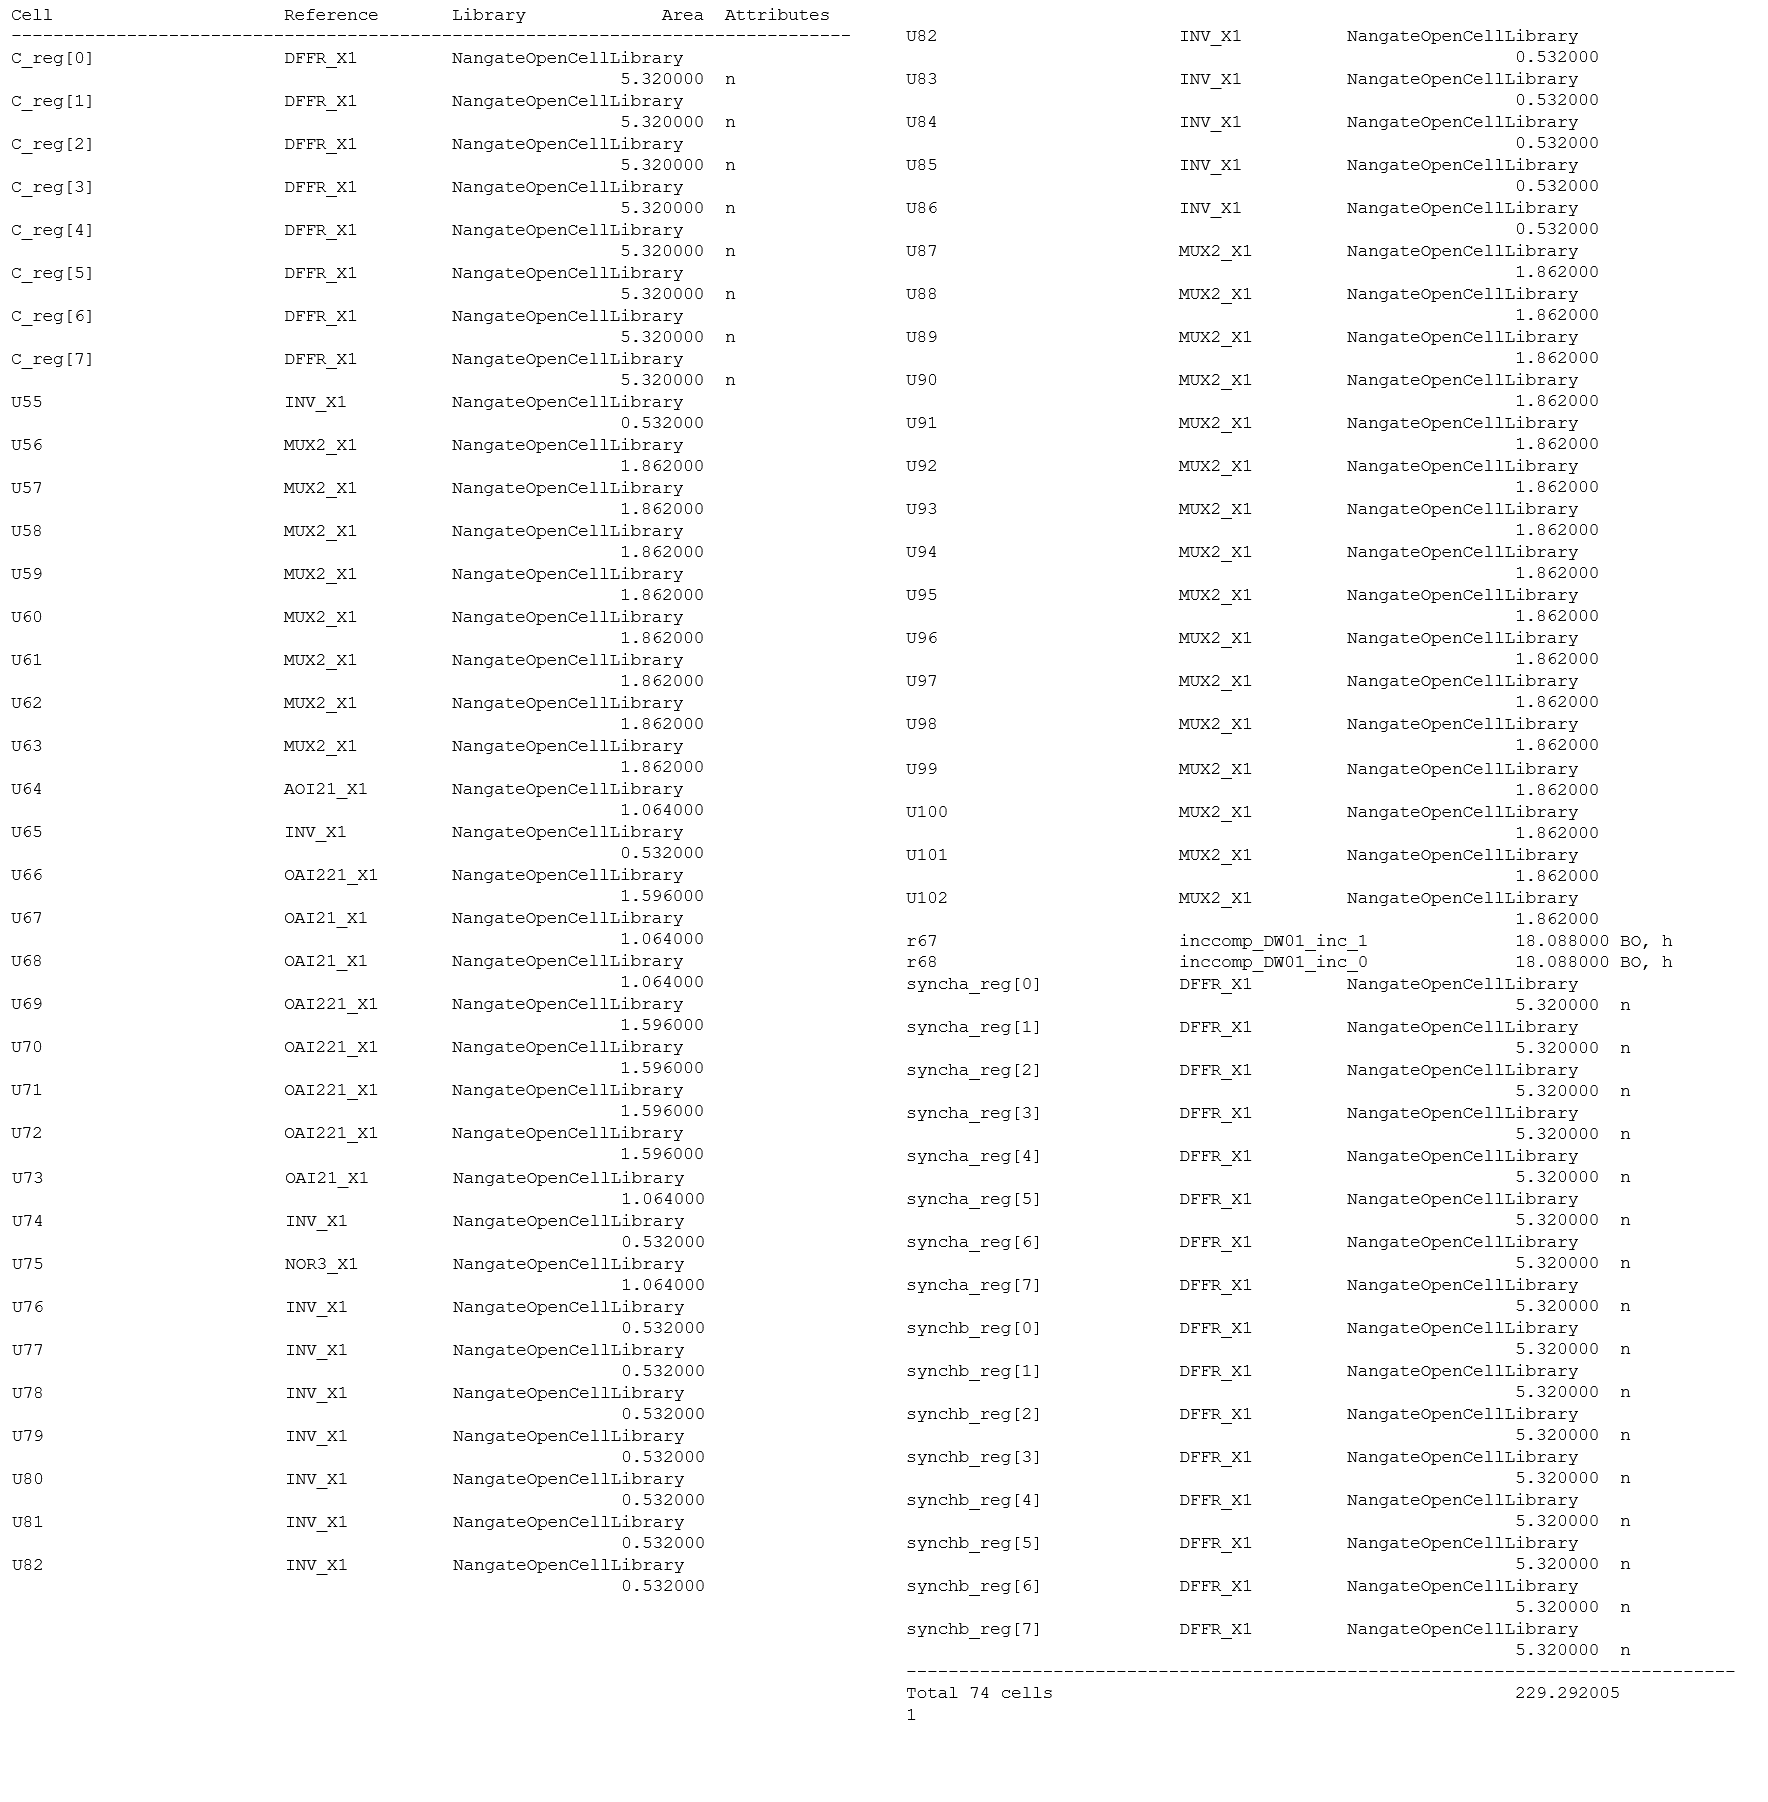
\includegraphics[scale=0.65]{immagini/3_6}
	\caption{\textit{Schema implementativo della tecnica del Clock Gating}}
	\label{3_6}
\end{figure}
\newpage
Ora si ri-eseguono le medesime simulazioni, ma utilizzando il circuito dove è stato applicata la tecnica del Clock Gating. Inizialmente si sono lasciati tutti i parametri esattamente come la prima analisi, quindi tutte le probabilità pari a 0.5, e si è ottenuto comunque una potenza inferiore del 16\% rispetto al caso senza la tecnica del Clock Gating. Il tutto viene riportato in Figura \ref{3_7} e \ref{3_8}. \\
\begin{figure}[!htb]
	\centering
	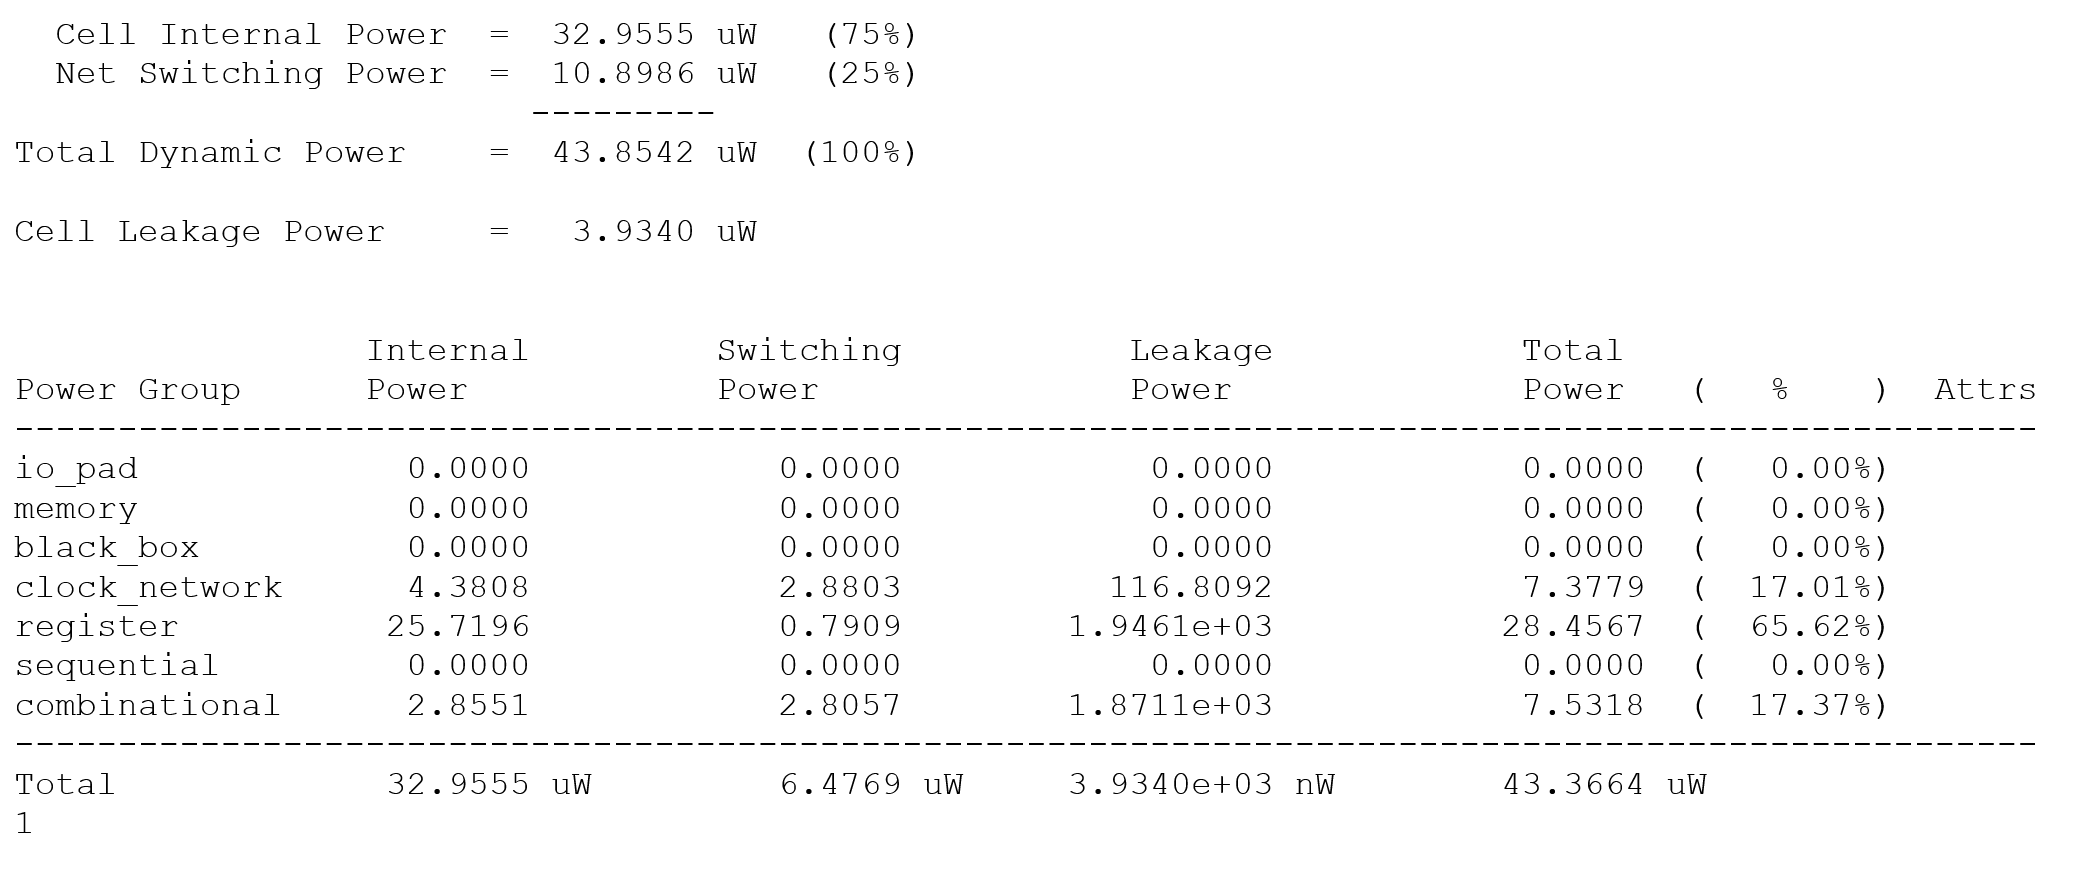
\includegraphics[scale=0.65]{immagini/3_7}
	\caption{\textit{Schema implementativo della tecnica del Clock Gating}}
	\label{3_7}
\end{figure}
\begin{figure}[!htb]
	\centering
	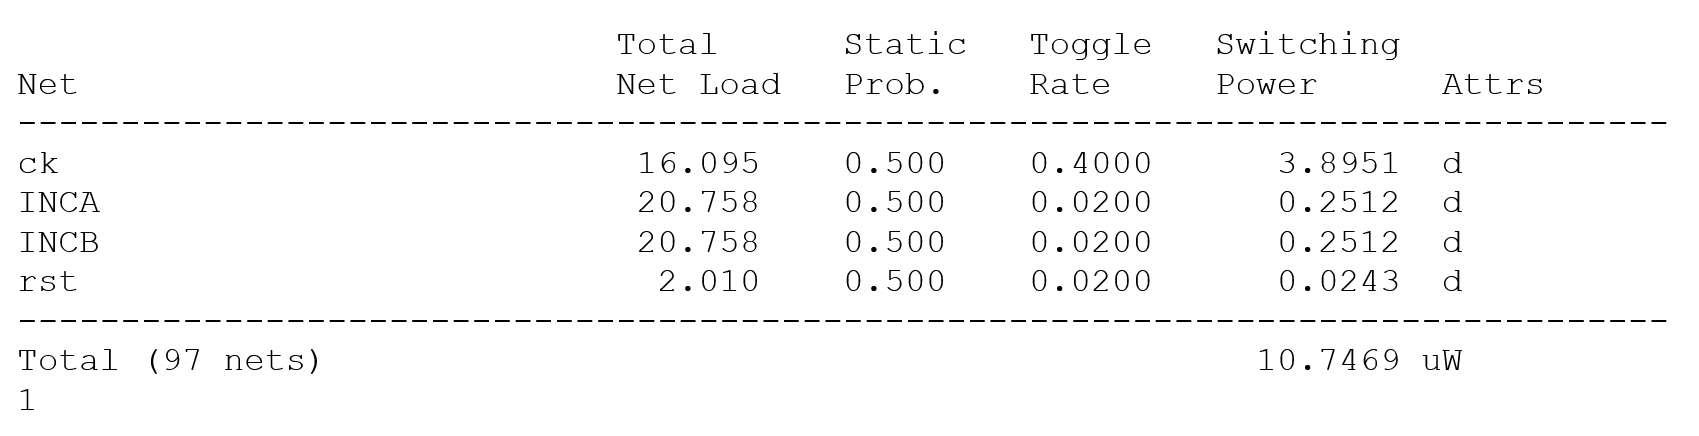
\includegraphics[scale=0.65]{immagini/3_8}
	\caption{\textit{Schema implementativo della tecnica del Clock Gating}}
	\label{3_8}
\end{figure}
\newpage
Esattamente come prima è stata cambiata la probabilità di reset, clock e input per vedere come cambiano i valori di potenza, portandole rispettivamente a 0, 0.5, 0.12.
Si è eseguito il comando \textit{report\_power -include\_input\_nets} e si sono analizzati i report di potenza che sono riportati in Figura \ref{3_9} e \ref{3_10}.\\
\begin{figure}[!htb]
	\centering
	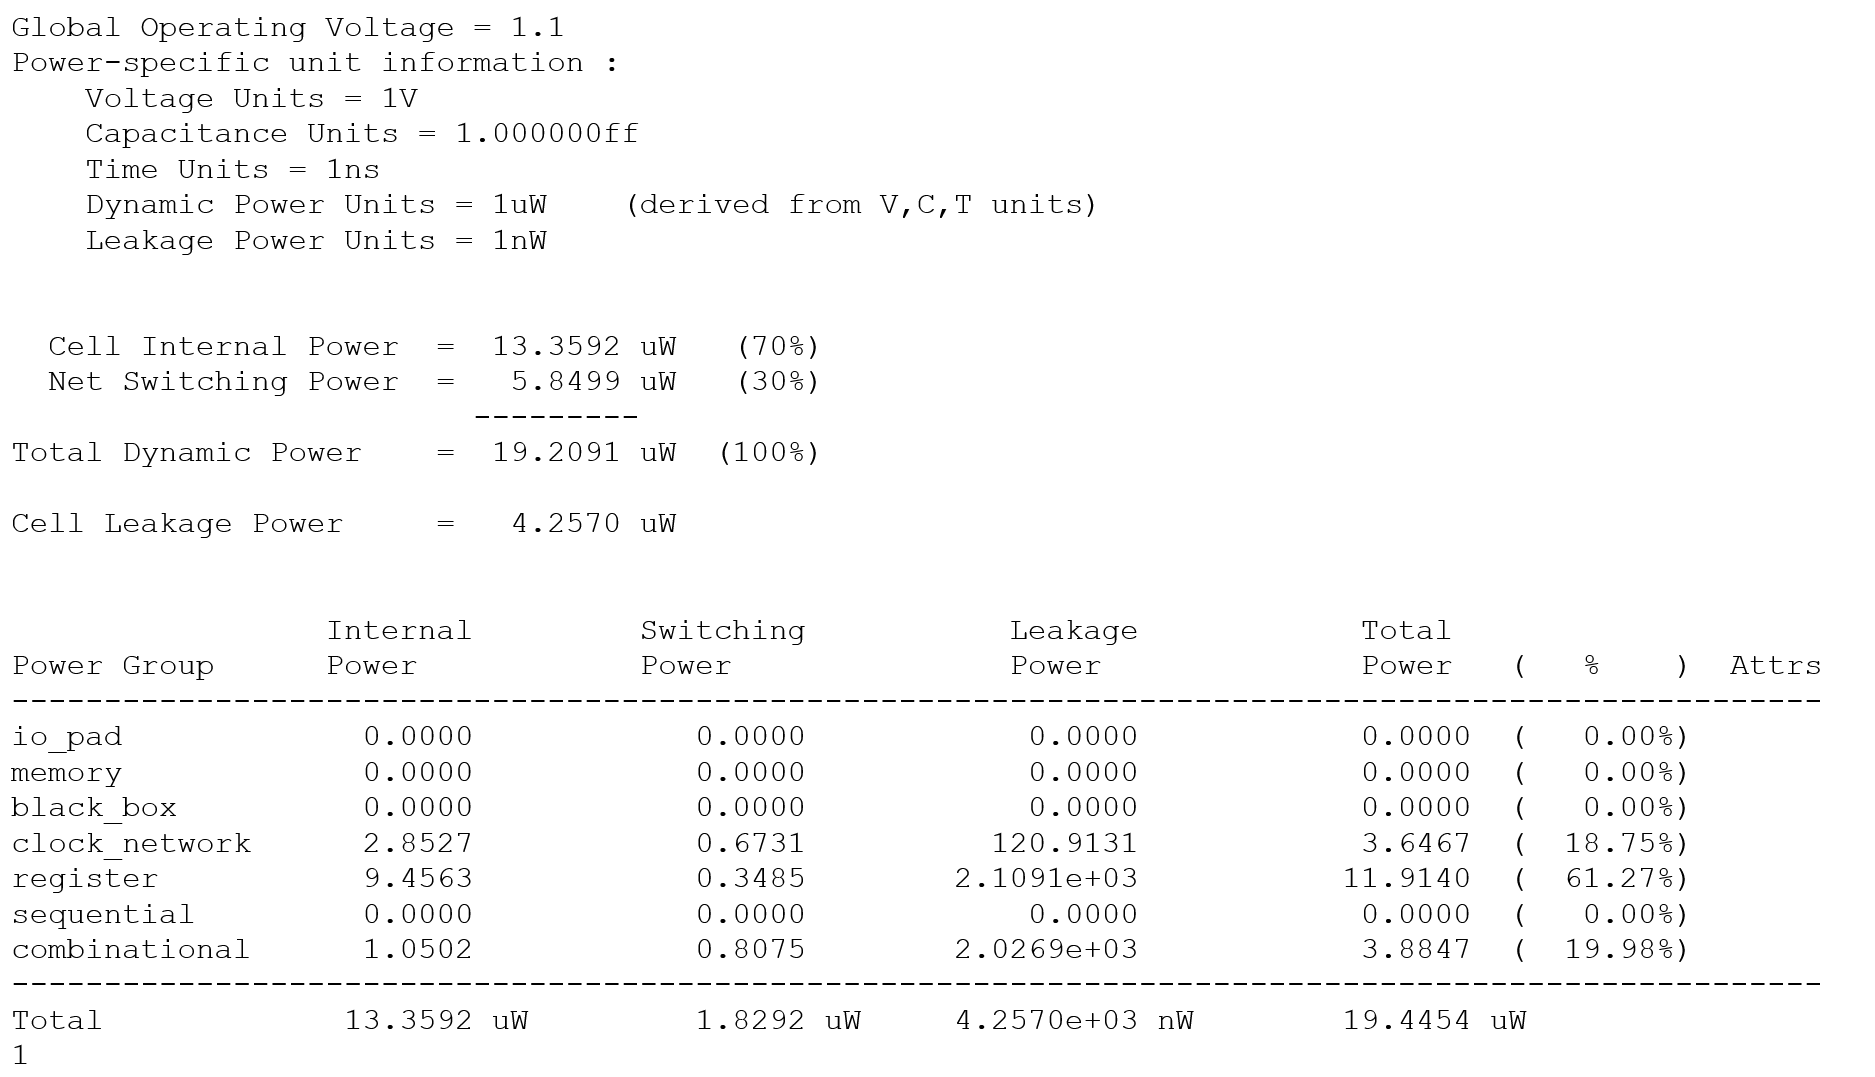
\includegraphics[scale=0.65]{immagini/3_9}
	\caption{\textit{Schema implementativo della tecnica del Clock Gating}}
	\label{3_9}
\end{figure}
\begin{figure}[!htb]
	\centering
	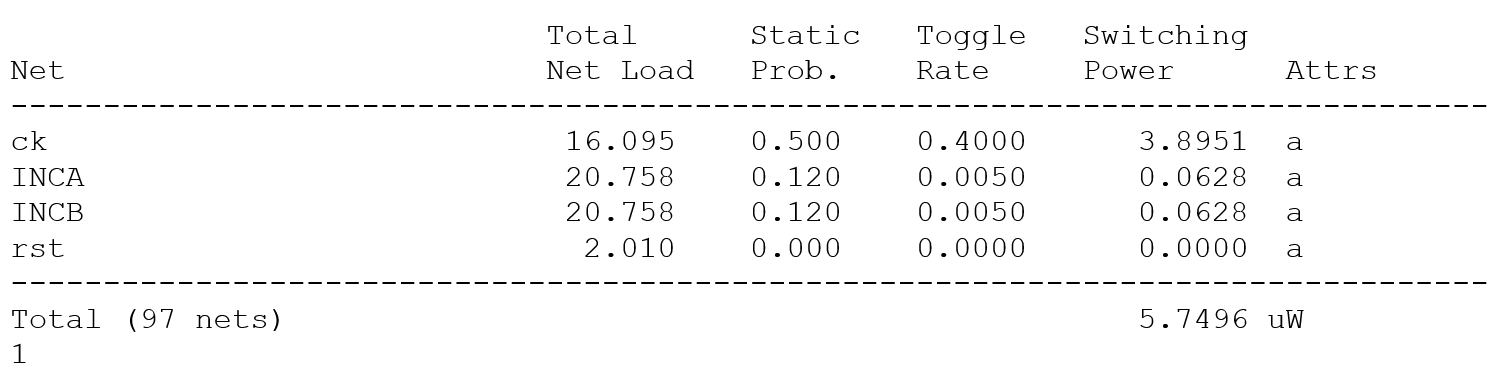
\includegraphics[scale=0.65]{immagini/3_10}
	\caption{\textit{Schema implementativo della tecnica del Clock Gating}}
	\label{3_10}
\end{figure}
\newpage

Si può notare come si è ottenuto un risparmio del 41\% rispetto al caso senza Clock Gating. \\
Infine si ri-esegue l'analisi tramite il report cell, raffigurato in Figura \ref{3_11}. Si può notare come ora il numero di celle sia aumentato e con esso anche l'area.\\
Rispetto al caso senza Clock Gating ho ora un'area pari a $238.0700005 \mu m^{2}$ e un numero di celle pari a 78. L'aumento dell'area è uno degli svantaggi della tecnica che Clock Gating, ma comunque, in questa situazione, si tratta di un'incremento pari solo al 3.47\%, che risulta assolutamente accettabile visto che comporta un risparmio di potenza pari al 41\%.
\begin{figure}[!htb]
	\centering
	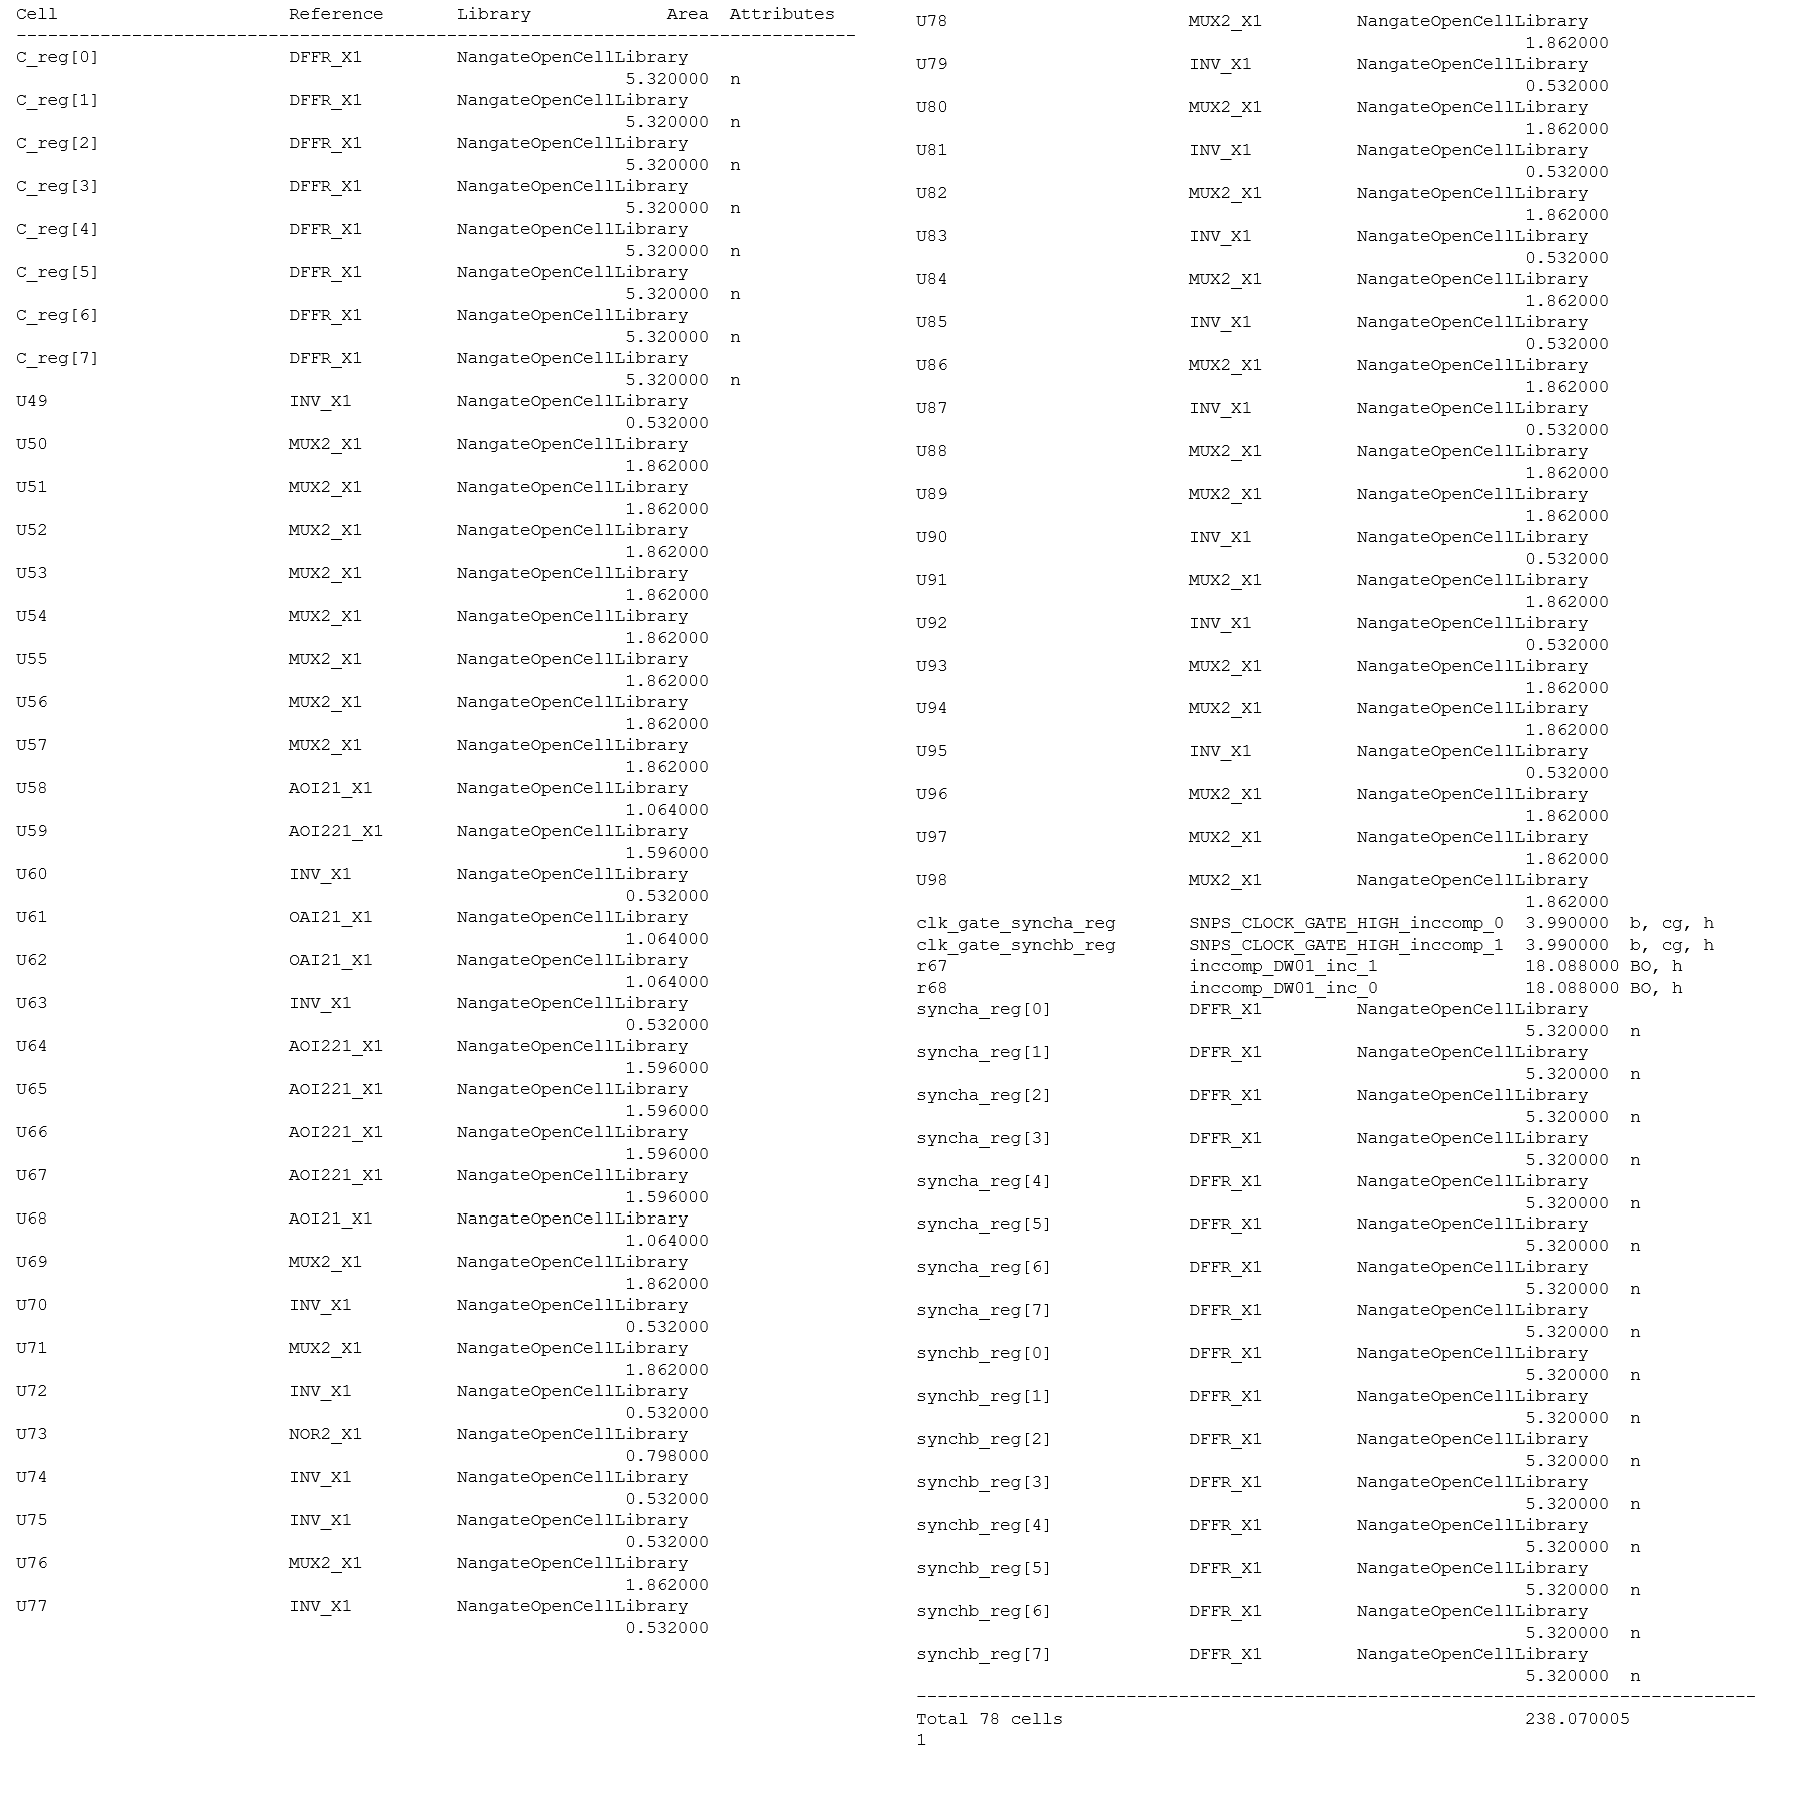
\includegraphics[scale=0.65]{immagini/3_11}
	\caption{\textit{Schema implementativo della tecnica del Clock Gating}}
	\label{3_11}
\end{figure}

\subsection{Some more clock gating?}
Il codice VHDL fornito è scritto in modo tale che il sintetizzatore non applichi la tecnica del Clock Gating sul registro di uscita: la motivazione risiede nell'utilizzo del costrutto \textit{if-else}, in quando nel codice iniziale non veniva dichiarati tutti i possibili casi tramite \textit{elsif}. Modificando opportunamente il codice VHDL,  riportato per interezza in appendice Figura \ref{3_vhdl}, e inserendo le linee di codice riportate in Figura \ref{3_vhdl_2}, il sintetizzatore inserisce un blocco di clock gating sul regitro di uscita perchè interpreta che potrebbero esserci condizioni in cui non si andrà a scrivere sul registro di uscita.
\begin{figure}[!htb]
	\centering
	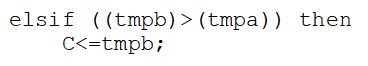
\includegraphics[scale=1.5]{immagini/3_vhdl_2}
	\caption{\textit{Schema implementativo della tecnica del Clock Gating}}
	\label{3_vhdl_2}
\end{figure}

\noindent Le modifiche al VHDL hanno portato al risultato richiesto, come si può notare in Figura \ref{3_12} che riporta il circuito sintetizzato e in Figura \ref{3_13} che riporta il particolare del blocco di Clock Gating inserito dal sintetizzatore.
\\
\begin{figure}[!htb]
	\centering
	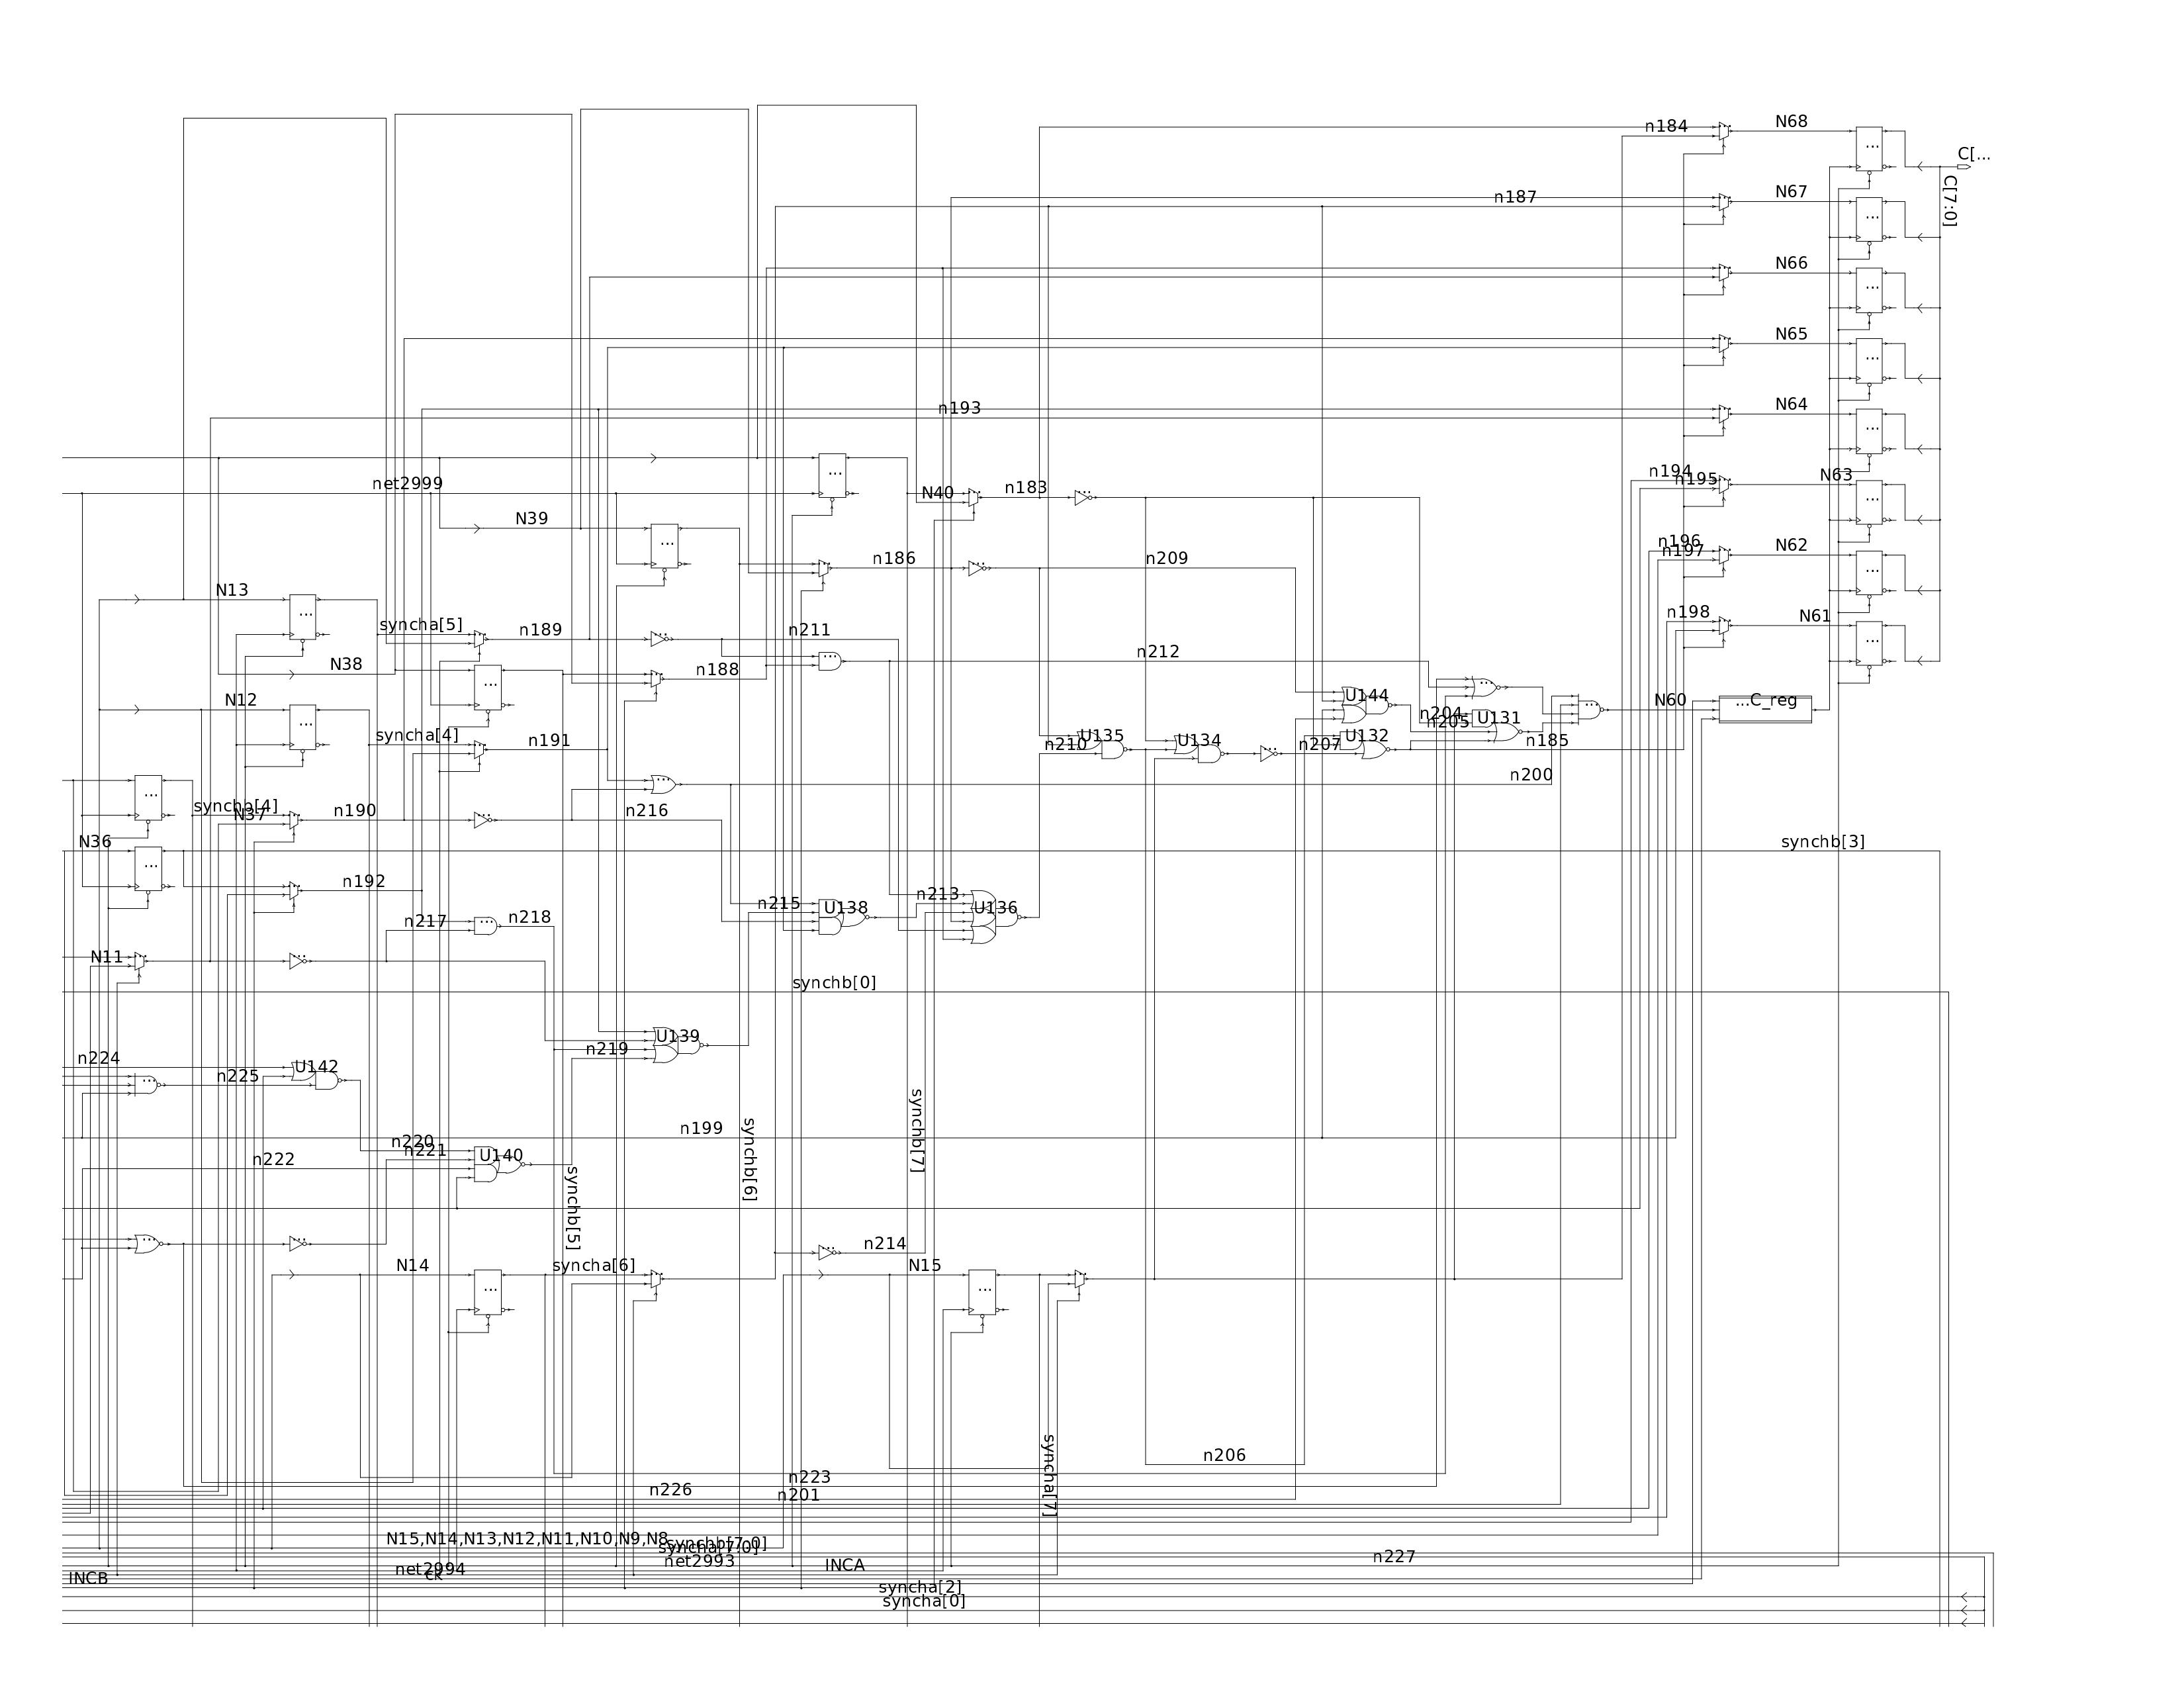
\includegraphics[scale=0.5]{immagini/3_12}
	\caption{\textit{Schema implementativo della tecnica del Clock Gating}}
	\label{3_12}
\end{figure}
\begin{figure}[!htb]
	\centering
	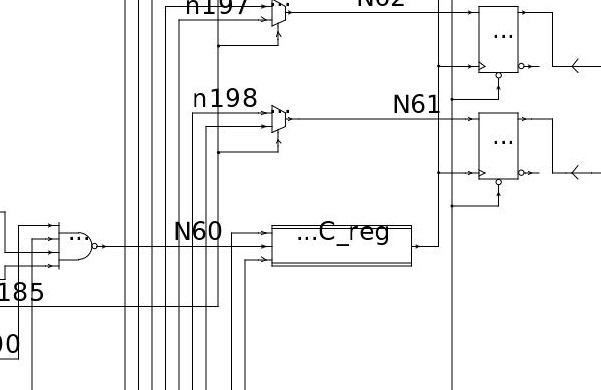
\includegraphics[scale=1.5]{immagini/3_13}
	\caption{\textit{Schema implementativo della tecnica del Clock Gating}}
	\label{3_13}
\end{figure}
\\
Si eseguono ora le analisi dei consumi, esattamente come nel punto precedente.\\
Le prima analisi viene svolta senza la tecnica del Clock Gating e vengono lasciati i valori di Toogle Rate di default, quindi a 0.5. I power report ricavati sono riportati in Figura \ref{elsif1} e \ref{elsif2}.
\begin{figure}[!htb]
	\centering
	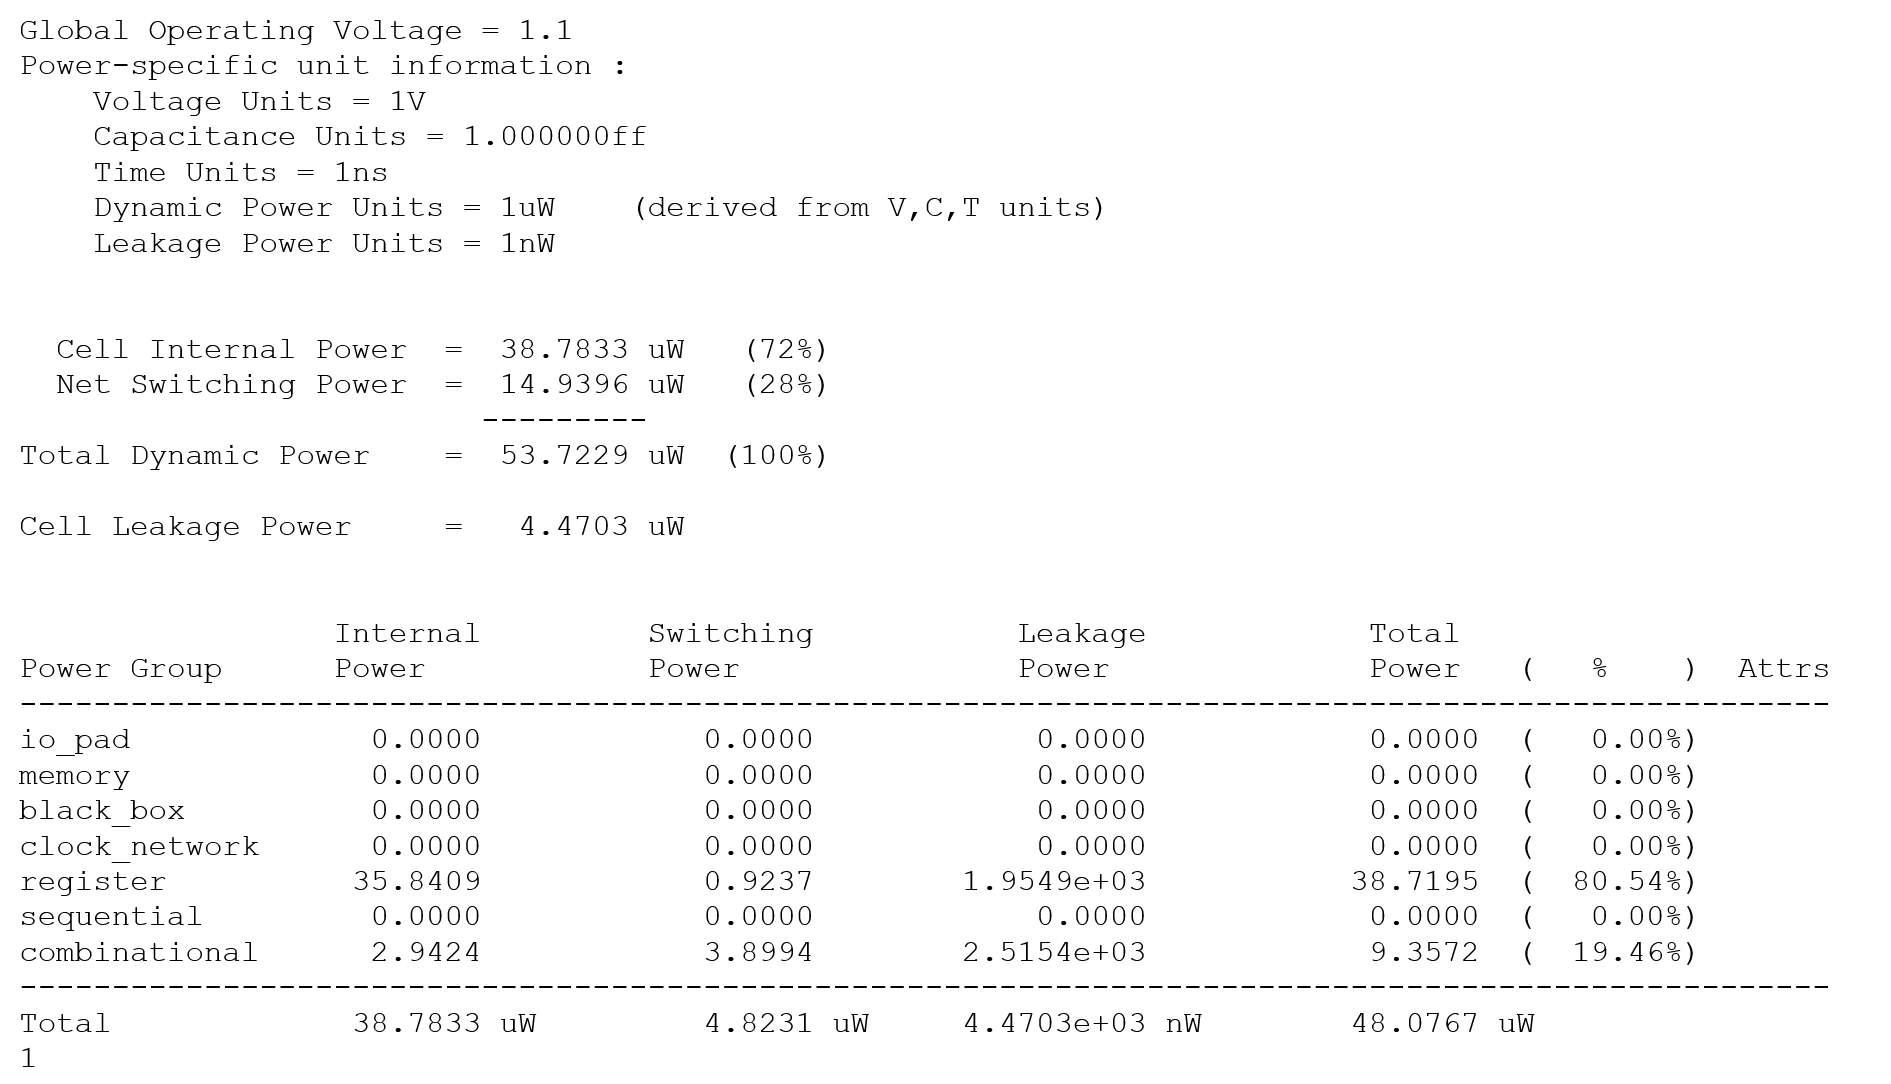
\includegraphics[scale=0.65]{immagini/elsif1}
	\caption{\textit{Schema implementativo della tecnica del Clock Gating}}
	\label{elsif1}
\end{figure}
\begin{figure}[!htb]
	\centering
	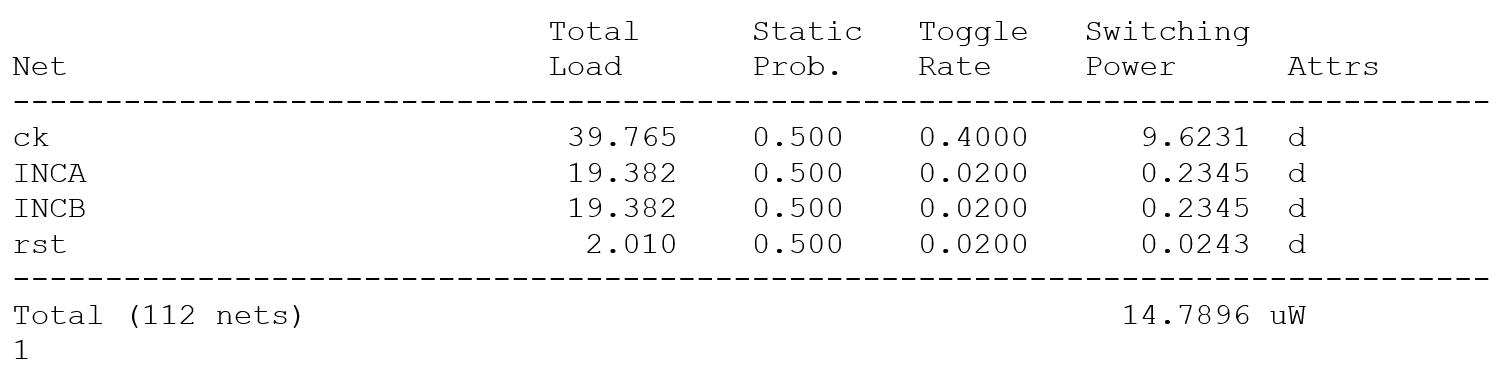
\includegraphics[scale=0.65]{immagini/elsif2}
	\caption{\textit{Schema implementativo della tecnica del Clock Gating}}
	\label{elsif2}
\end{figure}
Si può ben notare come rispetto al caso precedente, la potenza sia leggermente aumentata in quanto, avendo aggiunto un blocco di Clock Gating prima del registro di uscita, sono aumentati i gate totali che quindi portano ad una maggiore dissipazione di potenza. \\
Viene ora modificato il Toogle Rate del clock, del reset e degli ingressi, ottenendo i report in Figura \ref{elsif3} e \ref{elsif4}. L'aggiunta del blocco in uscita porta ad un primo risparmio di potenza pari a XX\% rispetto al caso analizzato al punto precedente. \\
\begin{figure}[!htb]
	\centering
	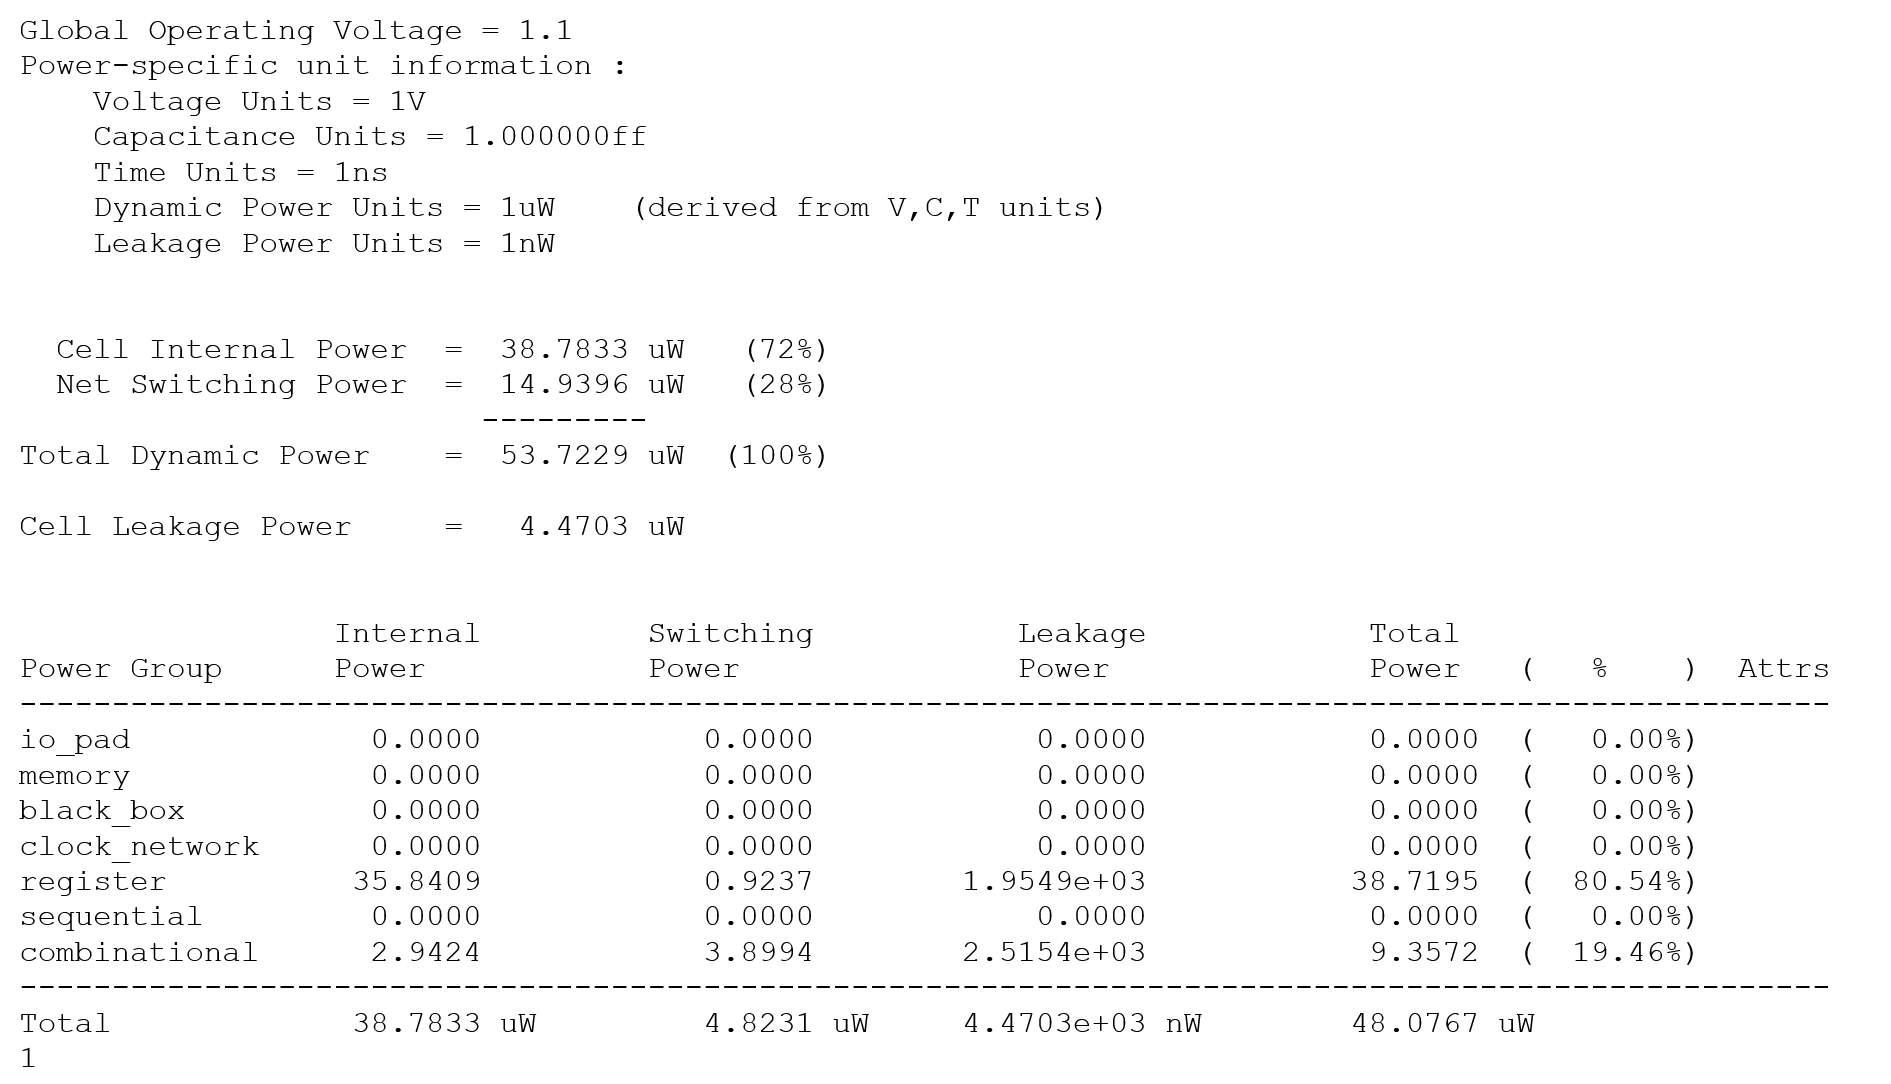
\includegraphics[scale=0.65]{immagini/elsif1}
	\caption{\textit{Schema implementativo della tecnica del Clock Gating}}
	\label{elsif3}
\end{figure}
\begin{figure}[!htb]
	\centering
	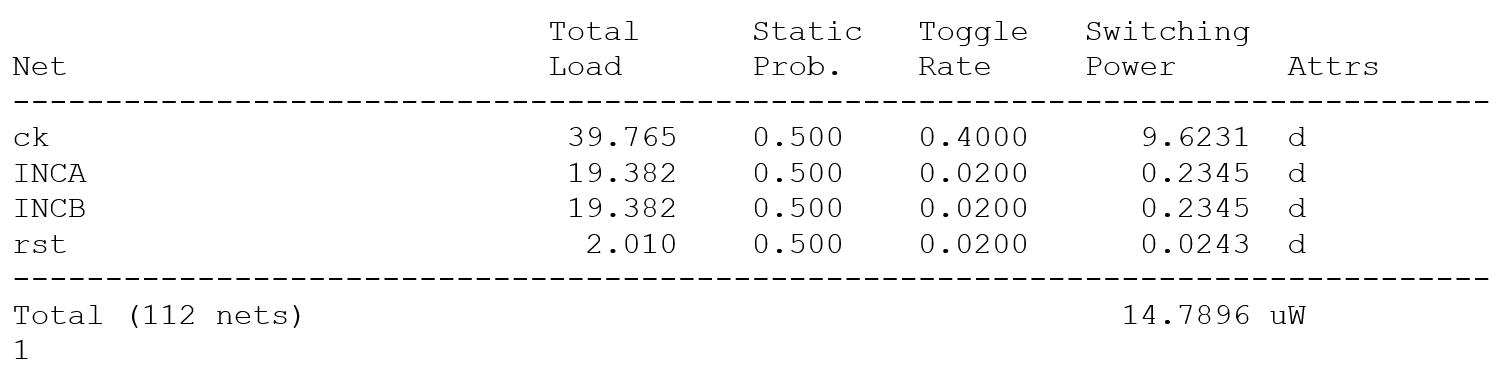
\includegraphics[scale=0.65]{immagini/elsif2}
	\caption{\textit{Schema implementativo della tecnica del Clock Gating}}
	\label{elsif4}
\end{figure}
\\
Si esegue infine il comando \textit{report cell} per ottenere l'area e il numero di celle utilizzate per la sintesi. Il report viene raffigurato i Figura \ref{elsif5}. \\
\newpage
\begin{figure}[!htb]
	\centering
	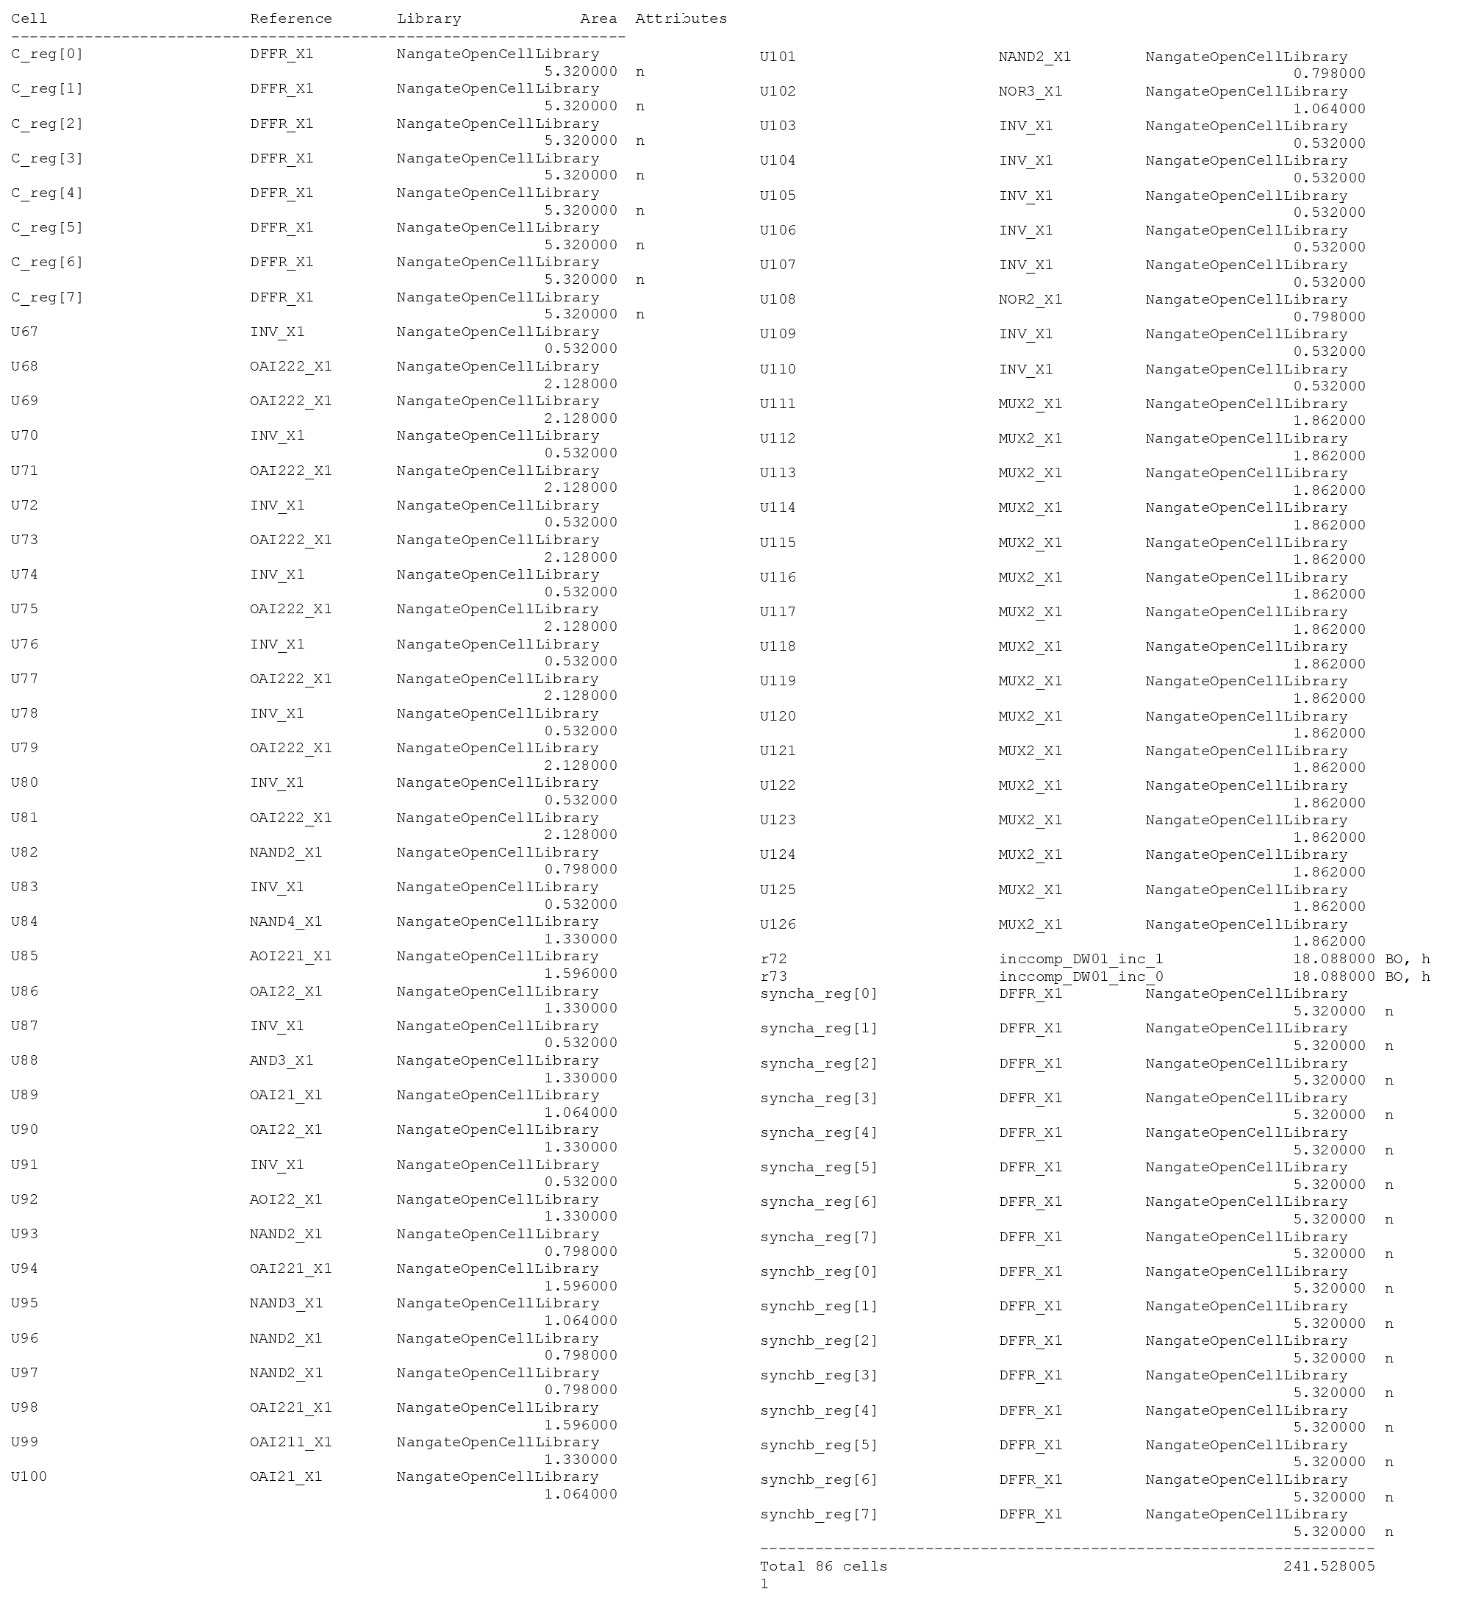
\includegraphics[scale=0.28]{immagini/elsif5}
	\caption{\textit{Schema implementativo della tecnica del Clock Gating}}
	\label{elsif5}
\end{figure}
\noindent Si può ben notare che ora il numero di celle è leggermente aumentato e di conseguenza anche l'area, in quanto si è aggiunta una logica prima del registro di uscita.\\
Si analizza allo stesso modo il circuito con l'aggiunta della tecnica del Clock Gating. Tutti i report, con lo stesso ordine dei punti precedenti, vengono riportati nelle Figure \ref{elsif6}, \ref{elsif7}, \ref{elsif8},\ref{elsif9}.\\
\begin{figure}[!htb]
	\centering
	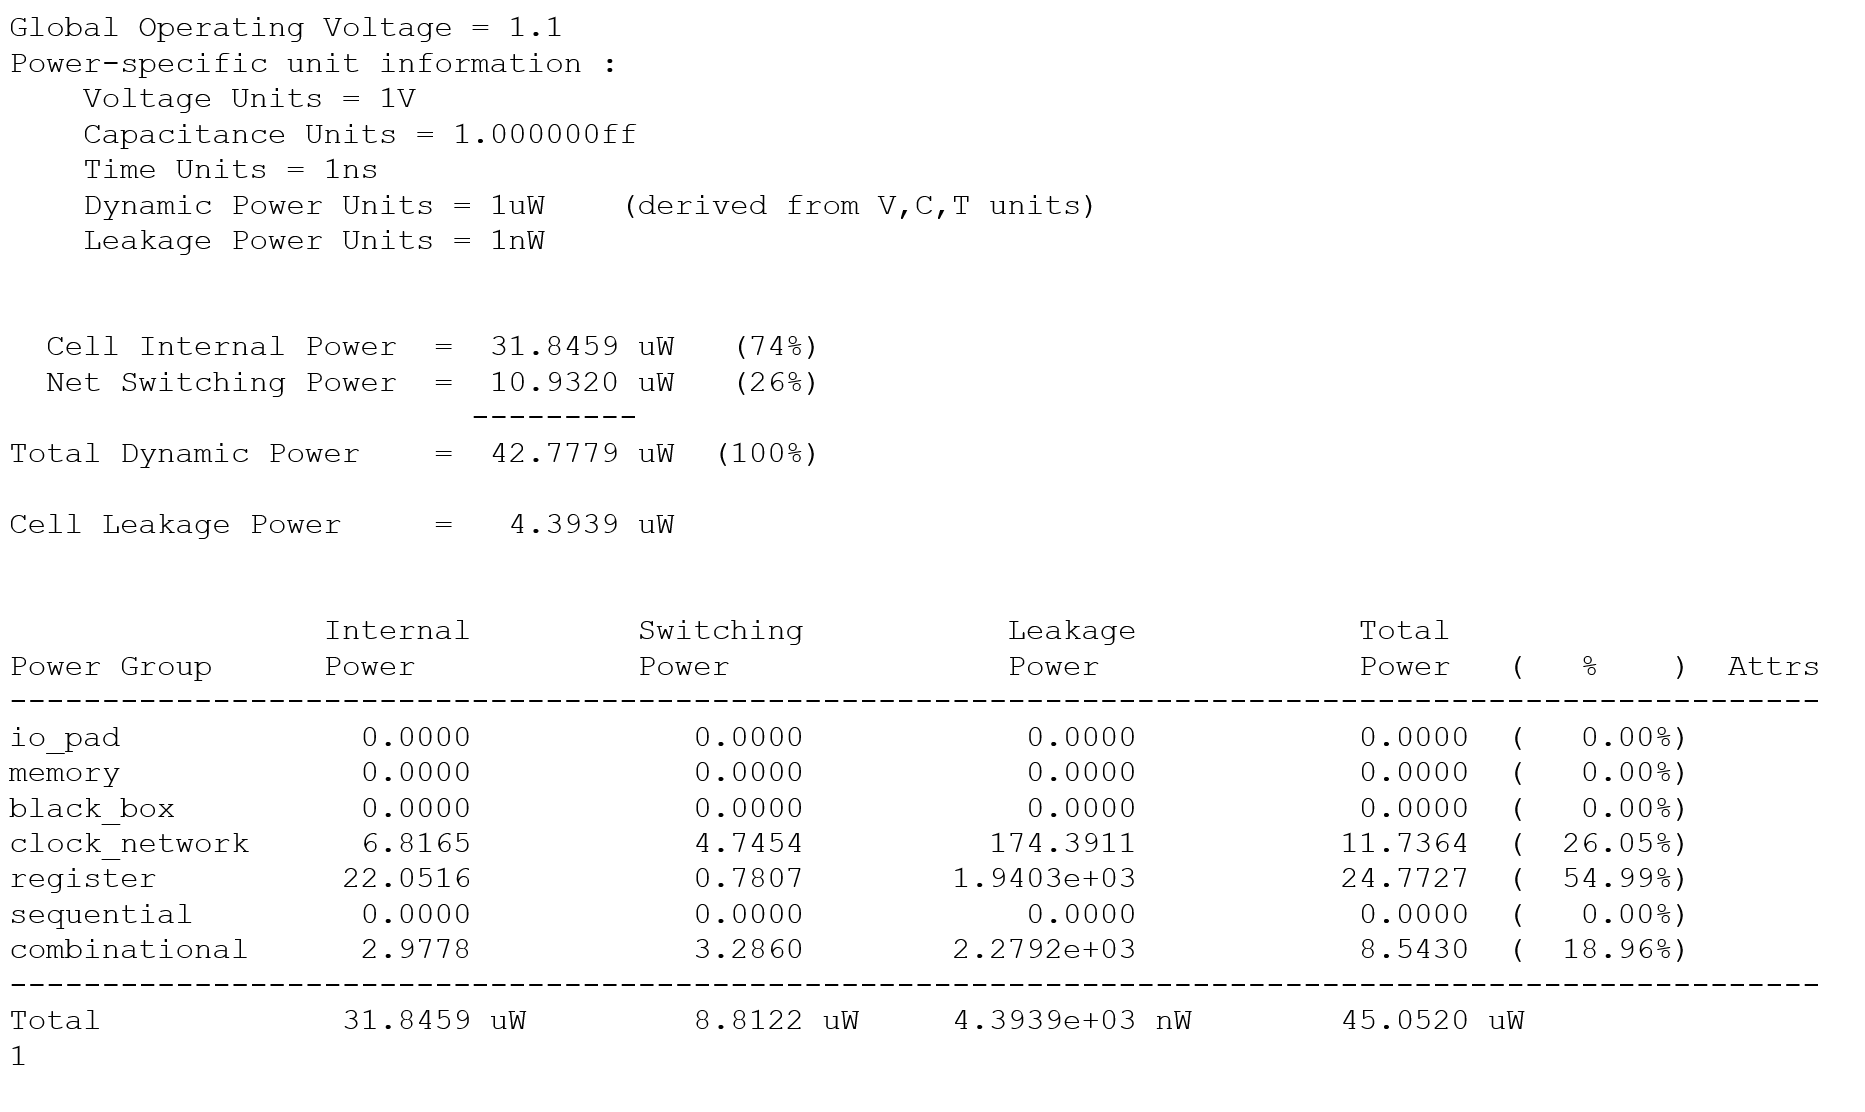
\includegraphics[scale=0.65]{immagini/elsif6}
	\caption{\textit{Schema implementativo della tecnica del Clock Gating}}
	\label{elsif6}
\end{figure}
\begin{figure}[!htb]
	\centering
	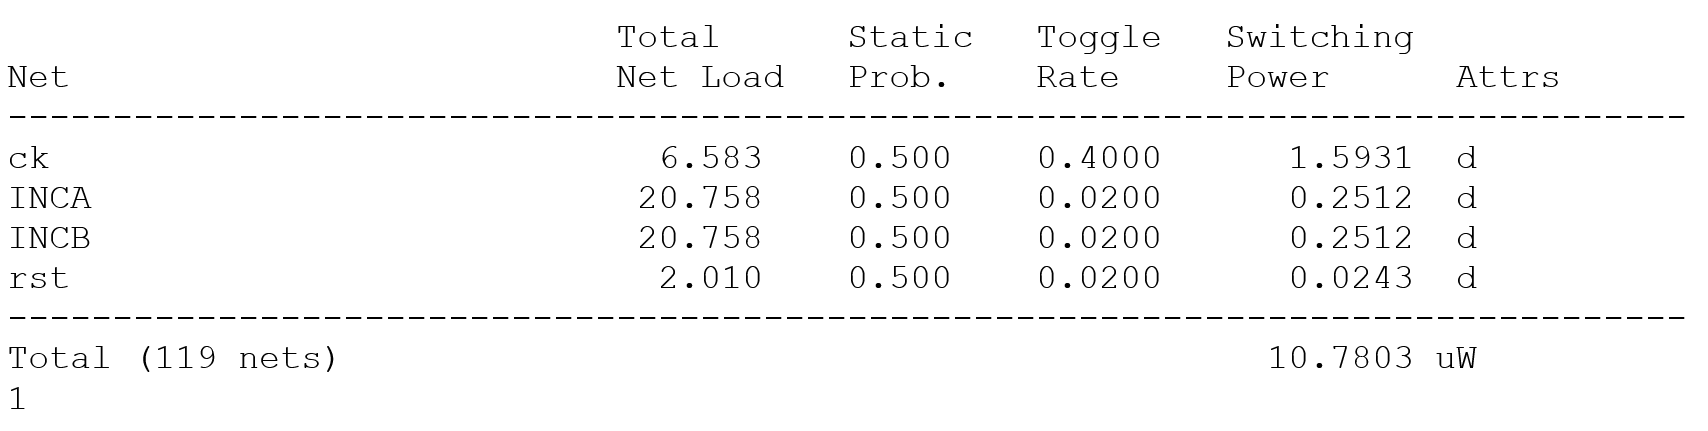
\includegraphics[scale=0.65]{immagini/elsif7}
	\caption{\textit{Schema implementativo della tecnica del Clock Gating}}
	\label{elsif7}
\end{figure}
\begin{figure}[!htb]
	\centering
	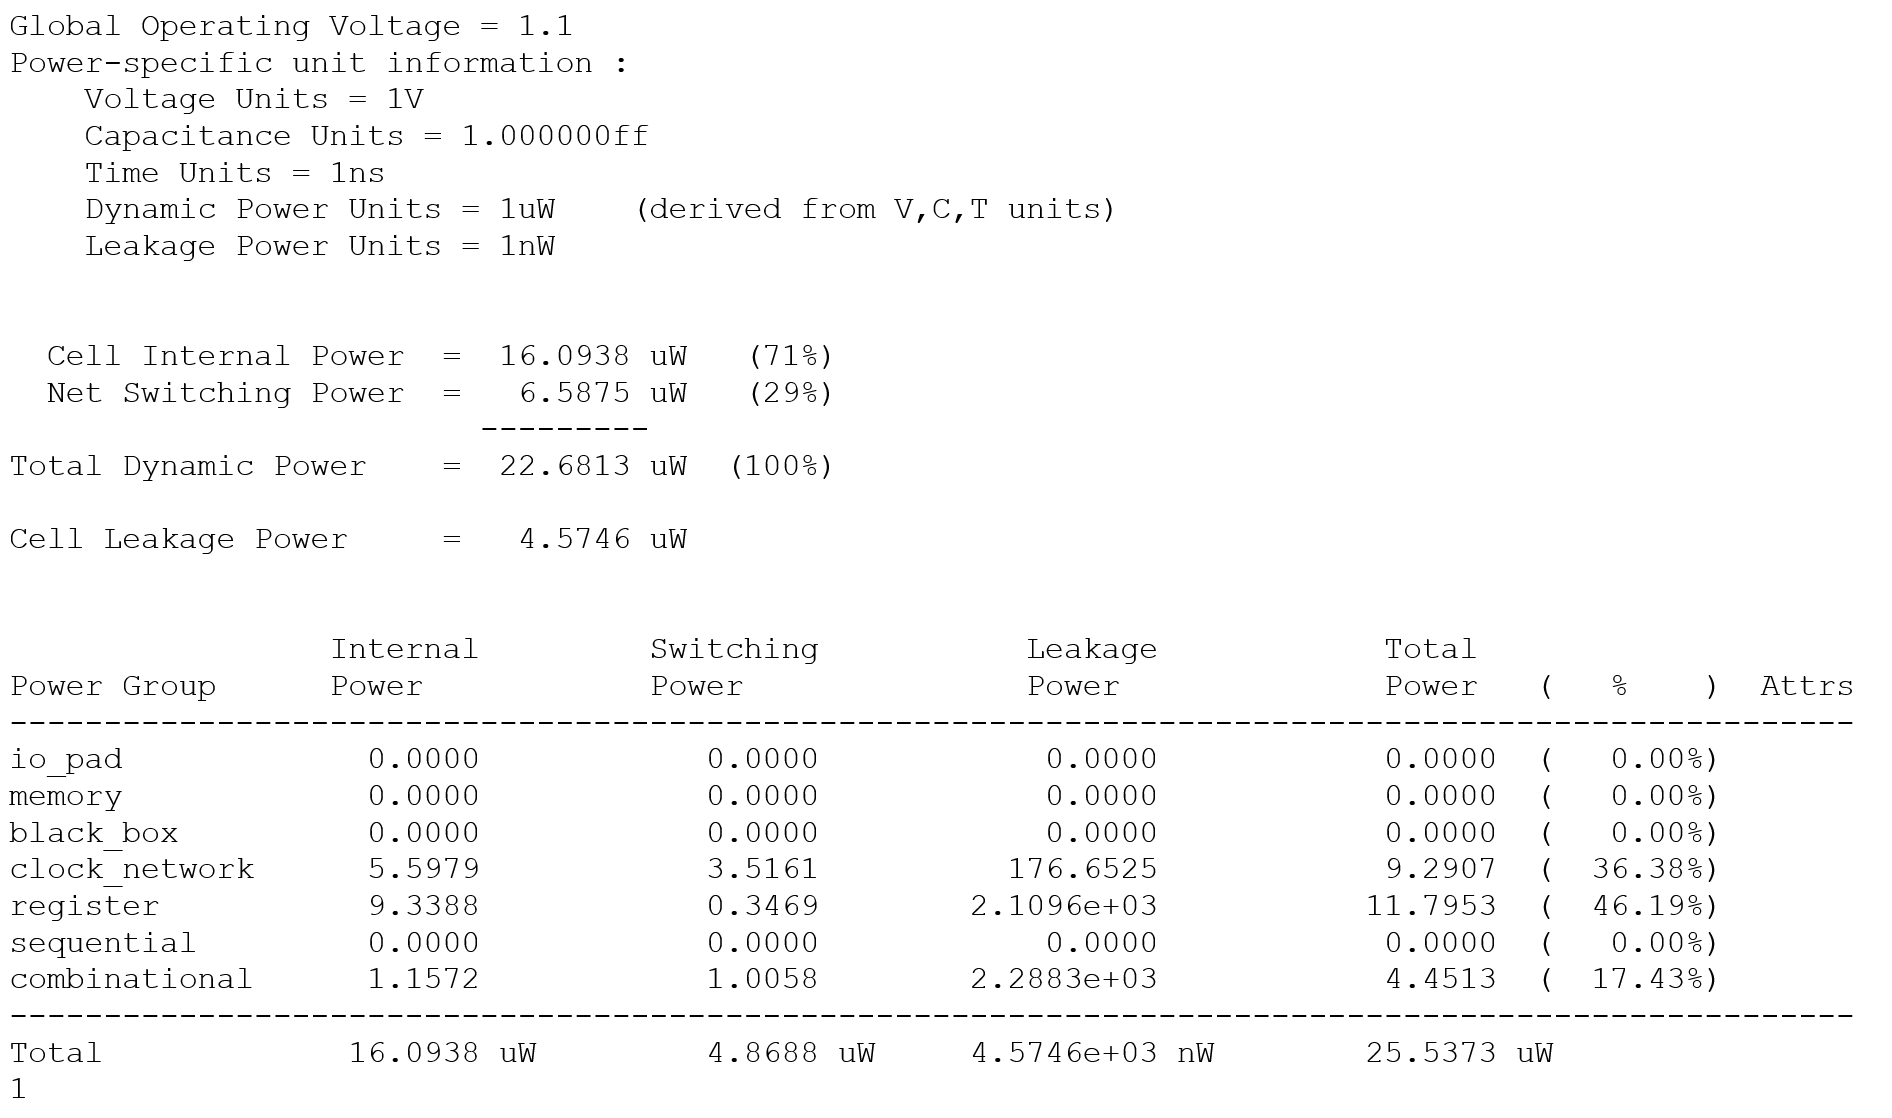
\includegraphics[scale=0.65]{immagini/elsif8}
	\caption{\textit{Schema implementativo della tecnica del Clock Gating}}
	\label{elsif8}
\end{figure}
\begin{figure}[!htb]
	\centering
	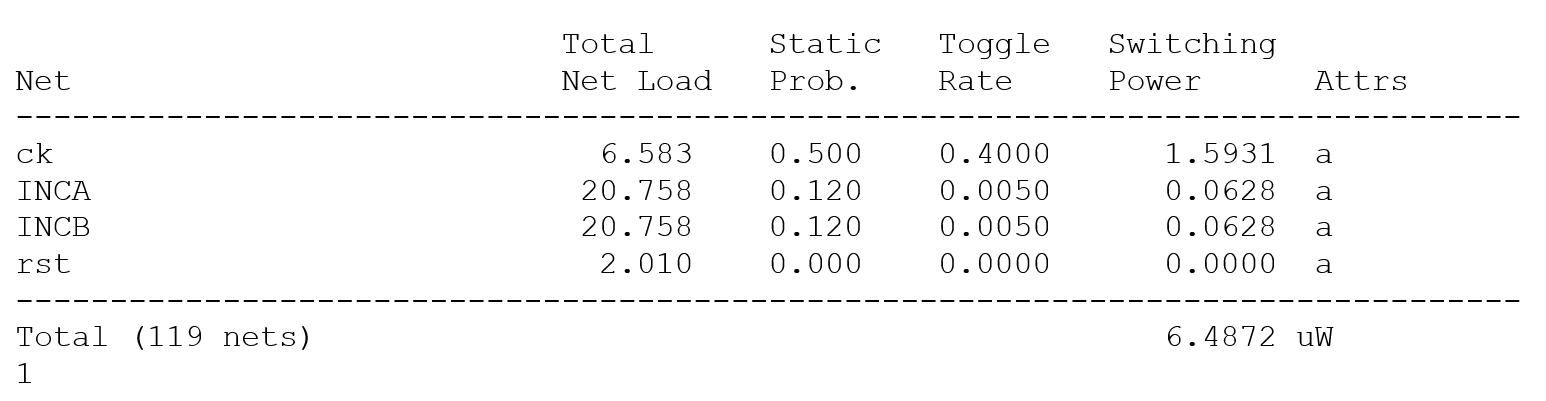
\includegraphics[scale=0.65]{immagini/elsif9}
	\caption{\textit{Schema implementativo della tecnica del Clock Gating}}
	\label{elsif9}
\end{figure}
\newpage
\noindent Si può ben notare come nell'ultimo caso, quindi con i Toogle Rate modificati rispetto ai valori di default, la potenza sia aumentata del 18\% rispetto al medesimo caso ma senza il blocco di Clock Gating prima del registro di uscita. Ovviamente se invece si confronta l'ultimo risultato con il risultato dell'analisi senza il Clock Gating, ma con il blocco in uscita, si ottiene un risparmio di potenza considerevole.\\
Come ultima analisi si esegue il \textit{report cell} di quest'ultimo caso, riportato in Figura \ref{elsif10}, che testimonia come l'applicazione di questa tecnica comporti un aumento dell'area occupata a causa dell'inserimeto di una logica di controllo.
\begin{figure}[!htb]
	\centering
	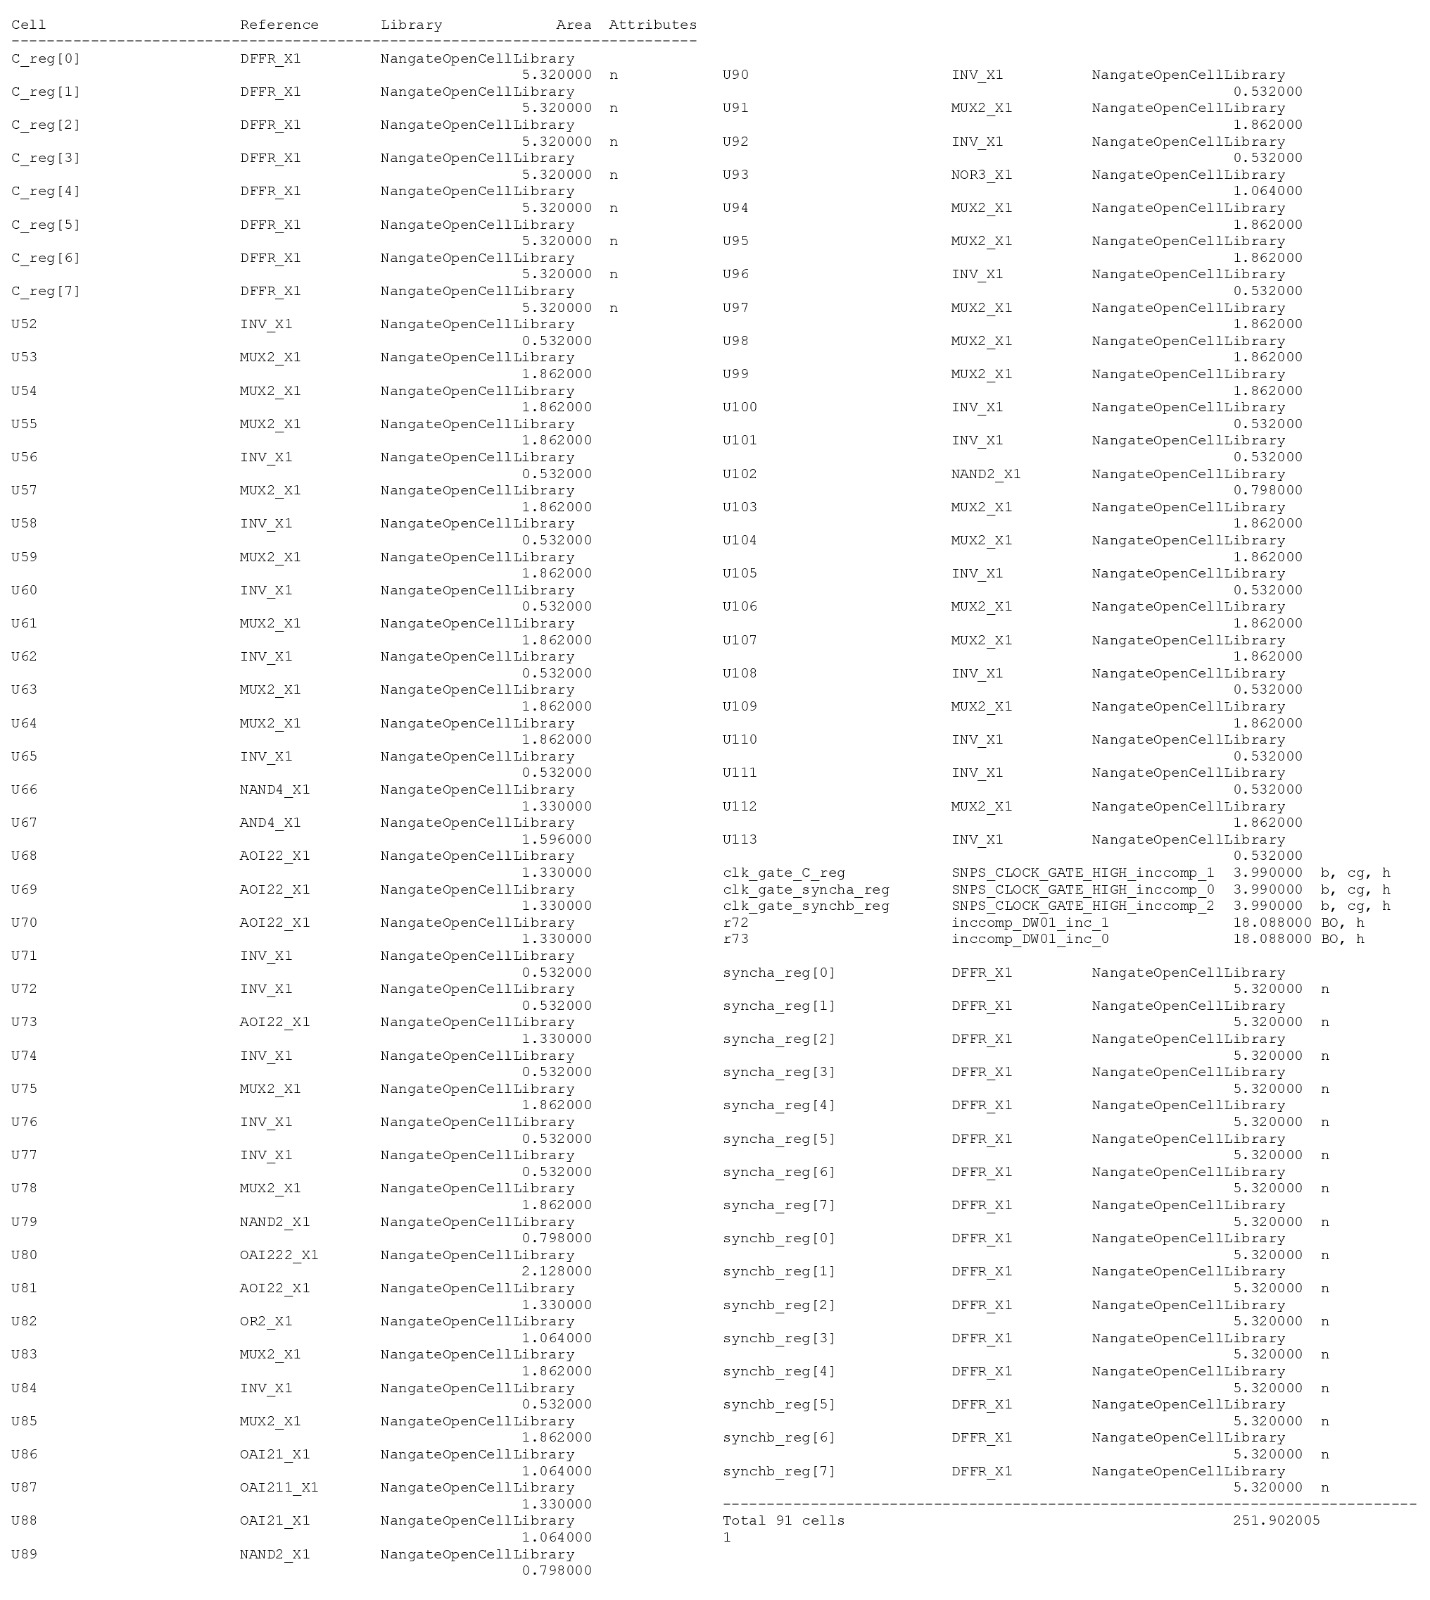
\includegraphics[scale=0.28]{immagini/elsif10}
	\caption{\textit{Schema implementativo della tecnica del Clock Gating}}
	\label{elsif10}
\end{figure}
\\
Per sintetizzare si confronta la potenza dinamica totale prima e dopo l'introduzione del Clock Gating nel registro di uscita e si riportano i valori nella Tabella \ref{Tab3_1}. Si può ben notare come la potenza nel secondo caso sia leggermente aumentata in quanto si introduce una logica di controllo più complessa che impatta sulla switching activity della macchina.
\begin{table}[!h]\footnotesize
	\centering
	\begin{tabular}{|c|c|}
		\hline
		& \textbf{Potenza Dinamica Totale}\\
		\hline
		Prima & $19.2091 \mu W$\\
		Dopo & $22.6813 \mu W$\\
		\hline
	\end{tabular}
	\caption{\textit{Risultati tempi NAND simulazione ELDO}}
	\label{Tab3_1}
\end{table}

\subsection{An automatic way to annotate activities}

\section{Pipelining and parallelizing}
Nella terza sezione dell'esercitazione si vede come si riesce a ridurre la potenza utilizzando la parallelizzazione e/o il pipelining. Si considera nuovamente il datapath del punto precedente, in Figura \ref{circuito_3_2}, di cui le caratteristiche di ritardo, potenza e occupazione di area sono riportate nella Tabella \ref{Tab33_1} nel caso in cui $V_{DD}=1 V$ e $f_{CLK}=5 MHz$.
\begin{table}[!h]\footnotesize
	\centering
	\begin{tabular}{|c|c|c|c|}
		\hline
		\textbf{Cell Type}& \textbf{Delay (ns)} & \textbf{Power ($\mu W @1 V, 5 MHz$)} & \textbf{Area ($\mu m^{2}$)} \\
		\hline
		\textit{REGISTER}& 2.0 (CK->Q) & 0.6 & 319 \\
	\textit{INCREMENT}& 40.0 & 2.55 & 256.0 \\
		\textit{COMPARATOR} & 84.0 & 2.16 & 161.0\\
		\textit{MUX} & 14.0 & 1.67& 117.0\\
		\hline
	\end{tabular}
	\caption{\textit{Risultati tempi NAND simulazione ELDO}}
	\label{Tab33_1}
\end{table}
\\
Utilizzando questi dati è possibile ricavare il percorso critico del circuito e da questo la massima frequenza di funzionamento.\\
Il percorso critico risulta essere causato dalla catena composta da registro di ingresso, incrementatore, comparatore, mux, registro di uscita. Viene allora calcolato il valore esatto del ritardo e la sua conseguente frequenza massima di funzionamento e da ciò si può ricavare anche la potenza totale consumata, in quanto esiste una dipendenza lineare tra potenza e frequenza. Tutti i dati sono raccolti in Tabella \ref{Tab33_2}.
\begin{table}[!h]\footnotesize
	\centering
	\begin{tabular}{|c|c|}
		\hline
		\textbf{Original Solution} & \\
		\hline
		Delay (critical path) & 142 ns\\
		Allowed Clock Frequency & 7.0422 MHz\\
		Power & $15.1125 \mu W$\\
		Area & $1747 \mu m^{2}$\\
		\hline
	\end{tabular}
	\caption{\textit{Risultati datapath "originale"}}
	\label{Tab33_2}
\end{table}
\newpage
\noindent Si prova ora a parallelizzare il circuito per ridurre il consumo di potenza ma avendo lo stesso throughput. Si duplica allora il datapath, raddoppiando dunque le capacità che commutano, ma si riesce a lavorare ad una frequenza dimezzata. Il nuovo circuito è raffigurato in Figura \ref{circuito_parallel}
\begin{figure}[!htb]
	\centering
	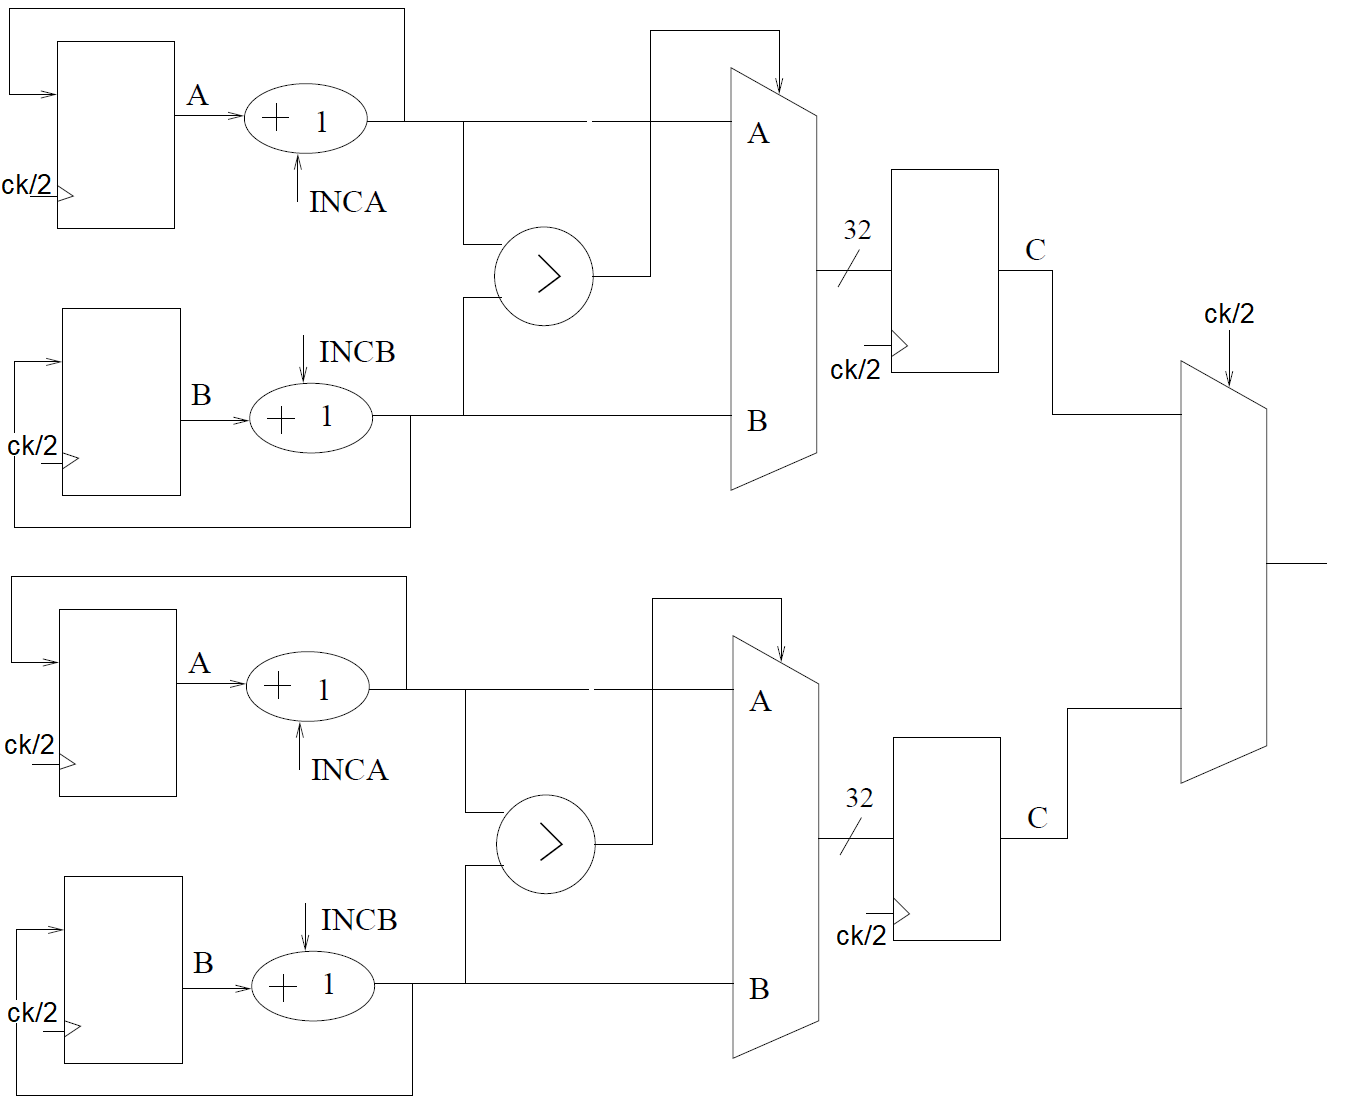
\includegraphics[scale=0.8]{immagini/circuito_parallel}
	\caption{\textit{Configurazione datapath con parallelizzazione a due livelli}}
	\label{circuito_parallel}
\end{figure}
\\
I due datapath lavorano dunque in parallelo, campionando uno sul fronte di salita del clock e l'altro sul fronte di discesa. Di conseguenza la frequenza operativa diventa ora esattamente la metà del caso precedente, dunque $f_{CK}=3.5211 MHz$ a cui corrisponde un periodo di clock pari a $T_{CK}=284 ns$. Ovviamente, nonostante la parallelizzazione, il percorso critico del circuito rimane pari a 140 ns e dunque si può pensare di allungarlo fino al valore del periodo del $T_{CK}$ in modo da poter scalare la tensione di alimentazione $V_{DD}$.\\
Per il calcolo del nuovo valore di alimentazione, vengono fornite delle formule che legano il periodo di clock alla tensione di alimentazione normalizzata rispetto a quella nominale (contrassegnata dalla variabile $u$). Si riportano in seguito i calcoli sviluppati per ottenere la nuova tensione di alimentazione normalizzata:
\begin{center}
	$T(u)=T(V_{DD}=V_{DD, NORM})\frac{0.75u}{u-0.25}=284 ns \Longrightarrow$
\end{center}
\begin{center}
		$\Longrightarrow u=\frac{0.25T(u)}{T(u)-0.75T(V_{DD}=V_{DD,NORM})}\Longrightarrow$
\end{center}
\begin{center}
	$\Longrightarrow u=\frac{0.25\times 284}{284-0.75 \times 142}=0.4$
\end{center}
Ottenuto il valore $u=0.4$, si può ricavare la potenza dissipata da ogni componente tramite l'equazione:
\begin{center}
   $P(V_{DD,new})=P(V_{DD, NOM})\times u^{2}$
\end{center}
Dove per ottenere ottenere i valori di $P(V_{DD, NOM}$ alla frequenza desiderata, ossia $f_{CK}=3.5211 MHz$, si sfrutta la linearità tra potenza e frequenza.
\begin{center}
	$P(V_{DD, NOM})=P(@V_ {DD}=1 V, f_{CK}=5MHz)\times \frac{3.5211 MHz}{5MHz}$
\end{center}
Si riportano nella Tabella \ref{Tab33_3} i nuovi valori di potenza per ogni singolo blocco.\\
\begin{table}[!h]\footnotesize
	\centering
	\begin{tabular}{|c|c|}
		\hline
		\textbf{Cell Type} & \textbf{$P(V_{DD, new})$} \\
		\hline
		\textit{REGISTER} & $0.4225 \mu W \times 0.4^{2}=0.0676 \mu W$\\
		\textit{INCREMENT} & $1.7958 \mu W \times 0.4^{2}=0.2873 \mu W$\\
		\textit{COMPARATOR} & $1.5211 \mu W \times 0.4^{2}=0.2534 \mu W$\\
		\textit{MUX} &$1.1760 \mu W \times 0.4^{2}=0.1882 \mu W$\\
		\hline
	\end{tabular}
	\caption{\textit{Risultati datapath "originale"}}
	\label{Tab33_3}
\end{table}
\\
Nella Tabella \ref{Tab33_4}, sono riportati ora i risultati riferiti alla parallelizzazione del circuito.
\begin{table}[!h]\footnotesize
	\centering
	\begin{tabular}{|c|c|}
		\hline
		\textbf{Parallel Solution} & \\
		\hline
		Delay (critical path) & 284 ns\\
		Allowed Clock Frequency & 3.5211 MHz\\
		Power & $2.6262\mu W$\\
		Area & $3611 \mu m^{2}$\\
		\hline
	\end{tabular}
	\caption{\textit{Risultati datapath "parallelizzato"}}
	\label{Tab33_4}
\end{table}\\
Si può notare che tramite la tecnica della parallelizzazione si ottiene un risparmio dell'$82\%$ rispetto al caso originale, mentre l'area risulta all'incirca raddoppiata.
\\
Si prova ora ad applicare allo stesso modo la tecnica del pipelining che consiste nello spezzare i percorsi combinatori inserendo alcuni registri: in questo modo si riduce drasticamente il percorso critico. \\
Il nuovo circuito è rappresentato in Figura \ref{circuito_pipe}.
\begin{figure}[!htb]
	\centering
	\includegraphics[scale=0.8]{immagini/circuito_pipe}
	\caption{\textit{Configurazione datapath pipelining}}
	\label{circuito_pipe}
\end{figure}
\\
Con questa nuova configurazione il percorso critico diventa quello tra il secondo registro e il comparatore.
\begin{center}
	$T_{critico}=T_{CK->Q}+T_{COMP}=2 ns + 84 ns = 86 ns$
\end{center}
Con questo percorso critico si potrebbe arrivare ad una frequenza di clock pari a $f_{CK}=11.6279 MHz$, ma così facendo si otterrebbero miglioramenti solo nell'ambito della velocità di funzionamento del circuito. L'obiettivo è sfruttare il pipelining per ridurre il consumo senza aumentare le prestazioni: di conseguenza si lascia la frequenza pari a $f_{CK}=7.0422 MHz$. \\
In questo modo il percorso critico risulterà comunque pari sempre a $142 ns$ e si potrà scalare la tensione di alimentazione $V_{DD}$. \\ Si eseguono dunque gli stessi calcoli fatti per il caso della parallelizzazione.
\begin{center}
	$T(u)=T(V_{DD}=V_{DD, NORM})\frac{0.75u}{u-0.25}=142 ns \Longrightarrow$
\end{center}
\begin{center}
	$\Longrightarrow u=\frac{0.25T(u)}{T(u)-0.75T(V_{DD}=V_{DD,NORM})}\Longrightarrow$
\end{center}
\begin{center}
	$\Longrightarrow u=\frac{0.25\times 142}{142-0.75 \times 86}=0.4581$
\end{center}
\begin{center}
	$P(V_{DD,new})=P(V_{DD, NOM})\times u^{2}$
\end{center}
\begin{center}
	$P(V_{DD, NOM})=P(@V_ {DD}=1 V, f_{CK}=5 MHz)\times \frac{7.0422 MHz}{5MHz}$
\end{center}

\noindent Tutti i nuovi valori di potenza dissipata dei singoli blocchi vengono riportati nella Tabella \ref{Tab33_5}
\begin{table}[!h]\footnotesize
	\centering
	\begin{tabular}{|c|c|}
		\hline
		\textbf{Cell Type} & \textbf{$P(V_{DD, new})$} \\
		\hline
		\textit{REGISTER} & $0.0448 \mu W \times 0.4581^{2}=0.1773 \mu W$\\
		\textit{INCREMENT} & $3.5910 \mu W \times 0.4581^{2}=0.7536 \mu W$\\
		\textit{COMPARATOR} & $3.0422 \mu W \times 0.4581^{2}=0.6384 \mu W$\\
		\textit{MUX} &$2.3521 \mu W \times 0.4581^{2}=0.4936\mu W$\\
		\hline
	\end{tabular}
	\caption{\textit{Risultati datapath pipelinato}}
	\label{Tab33_5}
\end{table}

Nella Tabella \ref{Tab33_6}, sono riportati ora i risultati riferiti alla tecnica del pipelining applicata al circuito.
\begin{table}[!h]\footnotesize
	\centering
	\begin{tabular}{|c|c|}
		\hline
		\textbf{Parallel Solution} & \\
		\hline
		Delay (critical path) & 142 ns\\
		Allowed Clock Frequency & 7.0411 MHz\\
		Power & $4.0576\mu W$\\
		Area & $3342 \mu m^{2}$\\
		\hline
	\end{tabular}
	\caption{\textit{Risultati datapath "parallelizzato"}}
	\label{Tab33_6}
\end{table}\\
Si può ben notare come, grazie alla tecnica del pipelining si ottiene un risparmio del 73\% rispetto al caso "originale".\\ Confrontando le due tecniche si può notare come ci sia all'incirca un fattore 2 di differenza tra le potenze risultanti che rende più efficace il metodo della parallelizzazione rispetto al metodo del pipelining. Per quanto riguarda l'area occupata, le due tecniche risultano all'incirca equivalenti, in quanto portano ad un raddoppio dell'area rispetto al circuito originale.\\
Si può pensare ora di sfruttare entrambe le tecniche per scalare il percorso critico, facendolo passare da 86 ns a 284 ns in modo da poter ridurre ancora la tensione di alimentazione e di conseguenza la potenza consumata. Il nuovo circuito è rappresentato in Figura \ref{circuito_parallel_pipe}.
\begin{figure}[!htb]
	\centering
	\includegraphics[scale=0.8]{immagini/circuito_parallel_pipe}
	\caption{\textit{Configurazione datapath pipelining}}
	\label{circuito_parallel_pipe}
\end{figure}\\
I risultati di questo nuovo approccio, che vengono calcolati mediante i medesimi passaggi fatti in precedenza sono riportati nella Tabella \ref{Tab33_7}.
\begin{table}[!h]\footnotesize
	\centering
	\begin{tabular}{|c|c|}
		\hline
		\textbf{Parallel and Pipelining Solution} & \\
		\hline
		u &0.3525\\
		Delay (critical path) & 284 ns\\
		Allowed Clock Frequency & 3.5211 MHz\\
		Power & $2.2\mu W$\\
		Area & $7120 \mu m^{2}$\\
		\hline
	\end{tabular}
	\caption{\textit{Risultati datapath "parallelizzato e pipelinato"}}
	\label{Tab33_7}
\end{table}\\
Tuttavia si può notare come questa soluzione non sia ottimale, poiché si ottiene un risparmio di potenza all'incirca pari al caso "parallelizato", ma impiegando un'area due volte superiore.\\
Infine si è analizzato il caso in cui si parallelizzi il sistema a tre livelli, andando a lavorare su una frequenza pari a $f_{ck}/3$: si scala di conseguenza il percorso critico, portandolo a 426 ns e si può ridurre ulteriormente la tensione di alimentazione $V_{DD}$. Anche in questo caso si riportano esclusivamente i risultati dei calcoli in Tabella \ref{Tab33_8}. 
\begin{table}[!h]\footnotesize
	\centering
	\begin{tabular}{|c|c|}
		\hline
		\textbf{Parallel and Pipelining Solution} & \\
		\hline
		u &0.3333\\
		Delay (critical path) & 426 ns\\
		Allowed Clock Frequency & 2.347 MHz\\
		Power & $1.76596\mu W$\\
		Area & $5358 \mu m^{2}$\\
		\hline
	\end{tabular}
	\caption{\textit{Risultati datapath "parallelizzazione a tre livelli"}}
	\label{Tab33_8}
\end{table}\\
Si può concludere affermando che la soluzione che porti al minor consumo di potenza sia la parallelizzazione a tre livelli, che comporta una riduzione della potenza pari a circa 8 volte la potenza del caso "originale". L'unico svantaggio di questa soluzione è che comporta un'area tre volte superiore.\\
Se si vuole cercare un trade-off tra area e potenza, sicuramente la soluzione migliore è la parallelizzazione a due livelli, che comporta un risparmio di potenza di circa 6 volte rispetto al caso originario, utilizzando "solo" un'area due volte superiore.\\
\subsection{Are you sure it was correct?}
Nelle Figura \ref{Timing3_1} e \ref{Timing3_2}, sono riportati i timing diagram rispettivamente del circuito originale e del caso "parallelizzato".
\begin{figure}[!htb]
	\centering
	\includegraphics[scale=2]{immagini/3_timing2}
	\caption{\textit{Timing datapath "originale"}}
	\label{Timing3_1}
\end{figure}\\
\begin{figure}[!htb]
	\centering
	\includegraphics[scale=2]{immagini/3_timing2}
	\caption{\textit{Timing datapath "parallelizzato"}}
	\label{Timing3_2}
\end{figure}\\
Si può ben notare come l'uscita del datapath nel secondo caso non sia corretta. Questo errore è dovuto al fatto che nel circuito siano presenti dei loop: questo implica che l'elaborazione del dato $i+1-esima$ può dipendere dall'elaborazione $i-esima$ e dunque non può essere effettuata su un altro circuito, come nel caso della parallelizzazione.






	\chapter{Laboratorio 4: \\Bus Encoding}
Durante questa esperienza di laboratorio, viene chiesto di analizzare e di valutare alcune tecniche di bus encoding. Nella prima parte dell'esperienza viene chiesto di valutare le performance delle varie tecniche in termini di transizioni e poi sintetizzare il sistema e verificare il consumo di potenza
\section{Simulation}
Durante la prima parte dell'esperienza viene chiesto di valutare, in termini di commutazioni, diverse tecniche di bus-encoding. Il tutto viene simulato grazie ad un testbench fornito e tramite i \textit{power report} generati da \textit{ModelSim}.
\subsection{Non-encoded}
Inizialmente si è simulato il caso in cui utilizzi un bus non codificato, andando a vedere l'evoluzione dei toogle in 10000 colpi di clock in modo tale da avere un punto di riferimento nel confronto con le altre varie tecniche. All'interno del testbench da simulare sono distinti due processi:
\begin{itemize}
	\item processo per gli indirizzi
	\item processo per i dati
\end{itemize}
i quali prendono come input i dati contenuti nel file \textit{rndin.txt} che, come sottolineato nella traccia, contiene delle stringe da 8 bit con un'alta probabilità di 1 logico. Questo fa già prevedere che la tecnica \textit{Transition-Based} risulterà meno performante, in quanto questa tipologia di codifica porta ad una riduzione delle commutazioni, solo nel caso in cui le probabilità di '1' logico siano molto più basse rispetto allo '0' logico.
Nelle Figure \ref{report_address_41} e \ref{report_dati_41}, sono riportati i \textit{power report} rispettivamente nel caso di dati e di indirizzi. Infine, nelle Tabelle \ref{Tab1} e \ref{Tab2} si riportano le switching activities rispettivamente nel caso di indirizzi e dati.
\begin{figure}[!htb]
	\centering
	\includegraphics[scale=0.65]{immagini/4_1_data_report}
	\caption{\textit{Power Report, tecnica no-encoding, caso 'data'}}
	\label{report_dati_41}
\end{figure}
\begin{table}[!h]\footnotesize
	\centering
	\begin{tabular}{|c|c|}
		\hline
		\textbf{Nodo} & \textbf{$E_{SW}$}\\
		\hline
		countbusnorm(7) & 0.0097\\
		countbusnorm(6) & 0.0118\\
		countbusnorm(5) & 0.0312\\
		countbusnorm(4) & 0.0624\\
		countbusnorm(3) & 0.1249\\
		countbusnorm(2) & 0.2499\\
		countbusnorm(1) & 0.4999\\
		countbusnorm(0) & 0.9999\\
		\hline
	\end{tabular}
	\caption{\textit{Switching Activity, tecnica no-encoding, caso 'data'}}
	\label{Tab1}
\end{table}
\newpage
\begin{figure}[!htb]
	\centering
	\includegraphics[scale=0.8]{immagini/4_1_addres_report}
	\caption{\textit{Power Report, tecnica no-encoding, caso 'address'}}
	\label{report_address_41}
\end{figure}
\begin{table}[!h]\footnotesize
	\centering
	\begin{tabular}{|c|c|}
		\hline
		\textbf{Nodo} & \textbf{$E_{SW}$}\\
		\hline
		countbusnorm(7) & 0.4974\\
		countbusnorm(6) & 0.5021\\
		countbusnorm(5) & 0.4987\\
		countbusnorm(4) & 0.4972\\
		countbusnorm(3) & 0.4959\\
		countbusnorm(2) & 0.4965\\
		countbusnorm(1) & 0.5023\\
		countbusnorm(0) & 0.506\\
		\hline
	\end{tabular}
	\caption{\textit{Switching Activity, tecnica no-encoding, caso 'address'}}
	\label{Tab2}
\end{table}
\subsection{Bus-invert technique, Transition based technique, Gray technique}
La codifica del Bus-invert consiste nel verificare che il dato successivo comporti un numero di commutazioni superiori di $\frac{N}{2}$, dove N è il numero di linee che compone il bus. In caso, conviene mandare il dato complementato e forzare ad '1' un bit denominato \textit{inv}, per segnalare che il dato in arrivo è in realtà complementato. Nelle Tabelle \ref{Tab3} e \ref{Tab4}, si riportano le Switching Activity rispettivamente nel caso di indirizzi e dati.\\
\begin{table}[!h]\footnotesize
	\centering
	\begin{tabular}{|c|c|}
		\hline
		\textbf{Nodo} & \textbf{$E_{SW}$}\\
		\hline
		countbusinv(8) & 0.0624\\
		countbusinv(7) & 0.0527\\
		countbusinv(6) & 0.0506\\
		countbusinv(5) & 0.0312\\
		countbusinv(4) & 0\\
		countbusinv(3) & 0.0625\\
		countbusinv(2) & 0.1875\\
		countbusinv(1) & 0.4375\\
		countbusinv(0) & 0.9375\\
		\hline
	\end{tabular}
	\caption{\textit{Switching Activity, tecnica bus-invert, caso 'address'}}
	\label{Tab3}
\end{table}
\begin{table}[!h]\footnotesize
	\centering
	\begin{tabular}{|c|c|}
		\hline
		\textbf{Nodo} & \textbf{$E_{SW}$}\\
		\hline
		countbusinv(8) & 0.365\\
		countbusinv(7) & 0.3576\\
		countbusinv(6) & 0.3611\\
		countbusinv(5) & 0.3617\\
		countbusinv(4) & 0.364\\
		countbusinv(3) & 0.3613\\
		countbusinv(2) & 0.3601\\
		countbusinv(1) & 0.3639\\
		countbusinv(0) & 0.3722\\
		\hline
	\end{tabular}
	\caption{\textit{Switching Activity, tecnica bus-invert, caso 'data'}}
	\label{Tab4}
\end{table}

\begin{figure}[!htb]
	\centering
	\includegraphics[scale=1.2]{immagini/transition}
	\caption{\textit{Schema tecnica 'Transition Based'}}
	\label{transition}
\end{figure}
\noindent Si esegue la medesima analisi per la tecnica \textit{Transition Based}, riportata in Figura \ref{transition}. Questa tecnica consiste nell'inviare uno '0' logico ogni qual volta la linea corrisponde alla precedente, mentre un '1' logico viene inteso come complemento del valore precedente della linea. I risultati delle simulazioni sono riportati per il caso dati in Tabella \ref{Tab5} e per il caso indirizzi in Tabella \ref{Tab6}. \\
\begin{table}[!h]\footnotesize
	\centering
	\begin{tabular}{|c|c|}
		\hline
		\textbf{Nodo} & \textbf{$E_{SW}$}\\
		\hline
		countbustran(7) & 0.5003\\
		countbustran(6) & 0.4946\\
		countbustran(5) & 0.4938\\
		countbustran(4) & 0.4997\\
		countbustran(3) & 0.5125\\
		countbustran(2) & 0.4989\\
		countbustran(1) & 0.500\\
		countbustran(0) & 0.4994\\
		\hline
	\end{tabular}
	\caption{\textit{Switching Activity, tecnica Transition-Based, caso 'data'}}
	\label{Tab5}
\end{table}
\begin{table}[!h]\footnotesize
	\centering
	\begin{tabular}{|c|c|}
		\hline
		\textbf{Nodo} & \textbf{$E_{SW}$}\\
		\hline
		countbustran(7) & 0.4816\\
		countbustran(6) & 0.3776\\
		countbustran(5) & 0.4992\\
		countbustran(4) & 0.4992\\
		countbustran(3) & 0.500\\
		countbustran(2) & 0.500\\
		countbustran(1) & 0.500\\
		countbustran(0) & 0.500\\
		\hline
	\end{tabular}
	\caption{\textit{Switching Activity, tecnica Transition-Based, caso 'address'}}
	\label{Tab6}
\end{table}
\begin{figure}[!htb]
	\centering
	\includegraphics[scale=1]{immagini/gray}
	\caption{\textit{Schema tecnica 'Codifica di Gray'}}
	\label{gray}
\end{figure}
\newpage
\noindent La tecnica \textit{Codifica di Gray}, riportata in Figura \ref{gray}: questa tecnica viene sfruttata specialmente nelle trasmissioni sequenziali, come ad esempio nel caso di indirizzi, in modo tale da cambiare esclusivamente un solo bit alla volta. I risultati delle Switching Activities sono riportati per i dati nella Tabella \ref{Tab7} e nella Tabella \ref{Tab8} per gli indirizzi. \\
\begin{table}[!h]\footnotesize
	\centering
	\begin{tabular}{|c|c|}
		\hline
		\textbf{Nodo} & \textbf{$E_{SW}$}\\
		\hline
		countbusgray(7) & 0.4974\\
		countbusgray(6) & 0.5087\\
		countbusgray(5) & 0.4952\\
		countbusgray(4) & 0.4981\\
		countbusgray(3) & 0.4937\\
		countbusgray(2) & 0.5056\\
		countbusgray(1) & 0.4962\\
		countbusgray(0) & 0.5075\\
		\hline
	\end{tabular}
	\caption{\textit{Switching Activity, tecnica Codifica di Gray, caso 'data'}}
	\label{Tab7}
\end{table}
\begin{table}[!h]\footnotesize
	\centering
	\begin{tabular}{|c|c|}
		\hline
		\textbf{Nodo} & \textbf{$E_{SW}$}\\
		\hline
		countbusgray(7) & 0.097\\
		countbusgray(6) & 0.055\\
		countbusgray(5) & 0.194\\
		countbusgray(4) & 0.312\\
		countbusgray(3) & 0.625\\
		countbusgray(2) & 0.125\\
		countbusgray(1) & 0.250\\
		countbusgray(0) & 0.500\\
		\hline
	\end{tabular}
	\caption{\textit{Switching Activity, tecnica Codifica di Gray, caso 'address'}}
	\label{Tab8}
\end{table}
\newpage
\noindent Si riportano per completezza i \textit{Power Report} delle simulazioni svolte con \textit{ModelSim}. In Figura \ref{address} si riporta il Report nel caso di indirizzi, mentre in Figura \ref{data} il caso di dati.
\\
\\
\begin{figure}[!htb]
	\centering
	\includegraphics[scale=1]{immagini/address_report_tecniche}
	\caption{\textit{Power Report complessivo, caso 'address'}}
	\label{address}
\end{figure}
\newpage
\begin{figure}[!htb]
	\centering
	\includegraphics[scale=0.8]{immagini/data_report_tecniche}
	\caption{\textit{Power Report complessivo, caso 'data'}}
	\label{data}
\end{figure}
\subsection{T0 techinque}
L'ultima tecnica richiesta è di implementare un codice per realizzare la tecnica \textit{T0 Encoding}. Nella traccia viene riportata la formula richiesta da implementare, riportata anche in Figura \ref{formula_t0}.\\
\begin{figure}[!htb]
	\centering
	\includegraphics[scale=0.8]{immagini/formula_t0}
	\caption{\textit{Formula implementata, tecnica 'T0'}}
	\label{formula_t0}
\end{figure}
\\
\noindent La codifica T0 consiste nell'inserire un bit in più, denominato \textit{INC}. Ogni volta che si va in sequenza, si forza questo segnale a '0' in modo tale che il ricevitore capisca di dover andare semplicemente in sequenza e si preoccupi lui di incrementare il dato. In caso di brach, salito o subroutine, forzo il segnale ad '1' e trasmetto sul bus il nuovo dato. Si riporta in appendice fig. \ref{t0} il \textit{Codice VHDL} dell'implementazione della codifica.
Sono state effettuate con modelsim le simulazioni di consumo di potenza e riportate di seguito rispettivamente per address fig. \ref{T0_address_power}   e data fig. \ref{T0_data_power} . 
\begin{figure}[!htb]
	\centering
	\includegraphics[scale=0.6]{immagini/T0_address_power}
	\caption{\textit{Power report T0, address}}
	\label{T0_address_power}
\end{figure}
\begin{figure}[!htb]
	\centering
	\includegraphics[scale=0.6]{immagini/T0_data_power}
	\caption{\textit{Power report T0, data}}
	\label{T0_data_power}
\end{figure}
\newpage
\subsection{Confronto tra le tecniche}
Confrontando i risultati tra le varie tecniche, si può notare come l'unica tecnica che porta ad una riduzione dei consumi nel caso dei dati, risulta essere la \textbf{Bus-Invert} con la quale si ottiene un risparmio sulle commutazioni pari a circa il 20\%. 
Per quanto concerne la tramissione di indirizzi, le codifiche più perfomanti risultano la \textbf{Codifica di Gray}, che porta ad un risparmio sulle commutazioni del 50\%, e la \textbf{Codifica T0}.
Si può notare come la tecnica che risulta meno performante è la \textbf{Transition Based}, che porta ad un incremento del 93\% nel caso di dati e ad un incremento circa del 0,1\% nel caso di indirizzi. Ovviamente questo è concorde con quanto ci si aspettava, in quanto, come già detto prima, questa tipologia di decofica funziona efficentemente solo nel caso in cui le probabilità di '1' e di '0' logico risultino sbilanciate.

\section{Synthesis}
Una volta aver stimato il consumo di potenza per la tecnica di bus non-encoded si può adesso calcolare i consumi per le quattro diverse tecniche di bus encoding, in presenza di due ingressi con diversa probabilità statistica: Address e Data.  
Per rendere più comoda e veloce la procedura sono stati utilizzati degli script, organizzati in modo da:
\begin{itemize}
\item{sintetizzare le architetture e salvarne il design (i file SDF e la netlist) tramite Synopsys}
\item{leggere i file SDF e simularli salvando i risultati in file VCD, poi convertiti in file SAIF per la backannotation, tramite il programma Modelsim}
\item{calcolare a partire dai file SAIF la sintesi del design e il consumo di potenza, tramite Synopsys}
\end{itemize}
Inoltre sono presenti dei file di configurazione contenenti variabili e opzioni per impostare lo script in base al tipo di simulazione richiesta.
Per entrambi i bus sono stati calcolati i consumi in  base a diversi carichi capacitivi alle linee di bus.
\\
\begin{table}[!h]\footnotesize
	\centering
	\begin{tabular}{|c|c|c|c|c|}
		\hline
		\textbf{uW} & \textbf{1fF} & \textbf{10fF} & \textbf{50fF} & \textbf{100fF}\\
		\hline
		normal & 10.158 & 11.387 & 16.220 & 23.236\\
		invert & 26.500 & 28.121 & 32.539  & 38.893\\
		transbased & 27.684 & 30.211 & 39.619 & 53.373\\
		gray & 9.440 & 10.059 & 12.496 & 16.012\\              
		t0 & 0.138 & 0.154 & 0. 220 & 0.316\\
		\hline
	\end{tabular}
	\caption{\textit{potenza dinamica dissipata nella trasmissione di indirizzi per le diverse codifiche in base al carico della linea.}}
\label{Tab9}
\end{table}
\\
Nel caso degli ADDRESS si può notare come la tecnica del T0 permette di ridurre i consumi di potenza dinamica di circa 10 volte, mentre la trans-based e la invert sono le peggiori.
\\
\begin{table}[!h]\footnotesize
	\centering
	\begin{tabular}{|c|c|c|c|c|}
		\hline
		\textbf{uW} & \textbf{1fF} & \textbf{10fF} & \textbf{50fF} & \textbf{100fF}\\
		\hline
		normal & 14.561 & 17.029 & 26.736 & 40.870\\
		invert & 36.643 & 38.460 & 46.385  & 57.812\\
		transbased & 26.628 & 29.114 & 38.929 & 53.082\\
		gray & 21.370 & 23.840 & 33.564 & 47.719\\              
		t0 & 17.298 & 20.106 & 29.503 & 44.776\\
		\hline
	\end{tabular}
	\caption{\textit{potenza dinamica dissipata nella trasmissione di dati per le diverse codifiche in base al carico della linea.}}
	\label{Tab10}
\end{table}
\\
Per quanto riguarda la trasmissione dei DATA invece, la codifica migliore dal punto di vista dei consumi si rivela essere la normal.
Chiaramente per entrambi gli ingressi e per qualsiasi codifica, è sempre valido il fatto che all'aumentare della capacità effettiva del bus i consumi di potenza dinamica aumentano, come dimostrano i risultati ottenuti.
\\

	\chapter{Laboratorio 5: \\Leakage: using spice for characterizing cells and pen\&paper for memory organization}
In questo laboratorio viene richiesto di analizzare i contributi di potenza, prestando particolare attenzione particolarmente alla potenza di leakage.

\section{Characterizing a library gate}
In questa prima parte dell'esercitazione viene richiesto di analizzare le performance di una \textit{NAND} a due ingressi, ottimizzata per essere \textit{High-Speed} per avere esattamente un punto di riferimento quando si analizzerà il caso con basso leakage. La porta NAND in questione si compone di due pMOS in parallelo, collegati alla Vdd e due nMOS in serie collegati al GND, come si può osservare in Figura \ref{nand_circuit}. \\
\begin{figure}[!htb]
	\centering
	\includegraphics[scale=0.3]{immagini/nand_circuit}
	\caption{\textit{Schema circuitale porta NAND}}
	\label{nand_circuit}
\end{figure}
La definizione del pMOS e dell'nMOS avviene tramite una piccola libreria \textit{'CMOS2013'}, all'interno della quale sono definiti i modelli che verranno analizzati (nel nostro caso si tratta del \textbf{EPHSGP\_BS2JU} per il pMOS e \textbf{ENHSGP\_BS2JU} per l'nMOS). All'interno di questa libreria ogni transistore viene identificato tramite alcuni parametri, quali la lunghezza e la larghezza del MOS e perimetri e aree di draine source.
L'analisi avviene tramite uno script \textit{'nandHS.sp'} che contiene una netlist dove vengono fissati i valori dei parametri di larghezza e lunghezza dei transitori.\\
Inoltre lo script contiene il alcuni comandi .measure tramite il quale vengono stimati i tempi di salita, di discesa e di propagazione della porta in questione. Viene richiesto di completare questi comandi andando a scrivere un comando per la misura tel tempo di propagazione basso-alto. Il comando aggiunto in questione è il seguente:
\begin{center}
\textit{.measure tran nanddelayHL TRIG V(inB) VAL='alim*0.5' RISE=1 
+ TARG V(out) VAL='alim*0.5' FALL=1}
\end{center}
Settando l'ambiente di simulazione \textbf{ELDO}, si può procedere con la simulazione della NAND in questione andando a riportare i parametri richiesti dalla traccia. Tra tutti i parametri viene richiesto ai annatore la potenza totale dissipata, che risulta essere pari a 6.7908 nW. I risultati temporali invece sono riportati in Tabella \ref{Tab5_1}.\\
\begin{table}[!h]\footnotesize
	\centering
	\begin{tabular}{|c|c|}
		\hline
		\textbf{Tempo} & \textbf{Misura}\\
		\hline
		$t_{rise}$ & 89.303 ps\\
		$t_{fall}$ & 74.319 ps\\
		$t_{pdHL}$ & 48.993 ps\\
		$t_{pdLH}$ & 56.490 ps\\
		\hline
	\end{tabular}
	\caption{\textit{Risultati tempi NAND simulazione ELDO}}
	\label{Tab5_1}
\end{table}
\\
Si possono confrontare questi valori andando ad avviare una simulazione grafica tramite \textbf{ezwave}. Le onde risultati sono riportate in Figura \ref{onde_5_1}, dove sono riportati i valori della due tensioni di ingresso che, come visto dalla netlist, risultano essere:
\begin{itemize}
	\item INA: costante al valore 1.2 V, assimilato come '1' logico
	\item INB: 0 V fino ad 1 ns, 1.2 V fino a 2 ns, 0 V fino al termine della simulazione
\end{itemize}
\begin{figure}[!htb]
	\centering
	\includegraphics[scale=0.35]{immagini/onde_5_1}
	\caption{\textit{Schema circuitale porta NAND}}
	\label{onde_5_1}
\end{figure}
Tramite gli appositi cursori del programma sono stati ricavati i tempi calcolati in precedenza con ELDO. Tutti i tempo sono riportati i Tabella \ref{Tab5_2}. 
\begin{table}[!h]\footnotesize
	\centering
	\begin{tabular}{|c|c|}
		\hline
		\textbf{Tempo} & \textbf{Misura}\\
		\hline
		$t_{rise}$ & 84.64 ps\\
		$t_{fall}$ & 74.01 ps\\
		$t_{pdHL}$ & 47.24 ps\\
		$t_{pdLH}$ & 56.71 ps\\
		\hline
	\end{tabular}
	\caption{\textit{Risultati tempi NAND simulazione ezwave}}
	\label{Tab5_2}
\end{table}
\\
Si può ben notare come i risultati siano assolutamente confrontabili.\\
In seguito viene chiesto di fare un analisi i continua, andando a decommentare alcune linee dello script, per andare a valutare le tensioni di soglia dei diversi MOS. I risultati sono riportati in Tabella \ref{Tab5_3}. 
\begin{table}[!h]\footnotesize
	\centering
	\begin{tabular}{|c|c|}
		\hline
		\textbf{Transistore} & \textbf{Tensione di Soglia $V_{TH}$}\\
		\hline
		VT(XNAND.XMN0.M1) & 0.31371 V\\
		VT(XNAND.XMN1.M1) & 0.27241 V\\
		VT(XNAND.XMP0.M1) & -0.24712 V\\
		VT(XNAND.XMP1.M1) & -0.24712 V\\
		\hline
	\end{tabular}
	\caption{\textit{Tensioni di soglia}}
	\label{Tab5_3}
\end{table}.
\\
Ovviamente, come ci si aspettava, le tensioni di soglia dei pMOS sono negative, mentre quelle degli nMOS sono positive. Le due tensioni di soglia dei pMOS risultano identiche; non vale lo stesso nel caso degli nMOS, in quanto si ha che la tensione di soglia del MOS0 è superiore alla tensione di soglia del MOS1. Questo genera di conseguenza una corrente di leakage più alta nel caso del MOS1 rispetto al MOS0.

\section{Characterizing a gate for output load}
L'obiettivo di questa seconda sezione dell'esercitazione è di analizzare il funzionamento della porta NAND andando a variare il carico in uscita. Si analizzano i casi con carico pari a:
\begin{itemize}
	\item 0.005 fF
	\item 0.05 fF
	\item 0.5 fF
	\item 5 fF
	\item 50 fF	
\end{itemize}
A tale scopo si analizzata, sempre tramite l'ambiente di simulazione \textit{ELDO}, il file \textit{nandHScharLoad.sp}. Rispetto al file precedente viene inserita una misura per valutare i picchi di corrente che scorrono nel GND e nella capacità di carico. I risultati della simulazione sono contenuti nella Tabella \ref{Tab5_4} per i tempi e nella Tabella \ref{Tab5_5} per i risultati legati alla corrente.
\begin{table}[!h]\footnotesize
	\centering
	\begin{tabular}{|c|c|c|c|c|c|}
		\hline
		\textbf{$C_{Load}$} & \textbf{0.005 fF} & \textbf{0.05 fF} & \textbf{0.5 fF} & \textbf{5 fF} & \textbf{50 fF}\\
		\hline
		$t_{rise}$ &67.226 ps &67.604 ps &71.228 ps &102.81 ps &363.91 ps \\
		
		$t_{fall}$ &68.551 ps &68.830 ps &72.112 ps &98.194 ps &296.52 ps \\
		
		$t_{pdHL}$&20.524 ps &20.851 ps &23.980 ps &48.550 ps &180.16 ps \\
		
		$t_{pdLH}$ &37.948 ps&38.286 ps &41.521 ps &66.657 ps &209.00 ps \\
		
		\hline
	\end{tabular}
	\caption{\textit{Tensioni di soglia}}
	\label{Tab5_4}
\end{table}.
\begin{table}[!h]\footnotesize
	\centering
	\begin{tabular}{|c|c|c|c|c|c|}
		\hline
		\textbf{$C_{Load}$} & \textbf{0.005 fF} & \textbf{0.05 fF} & \textbf{0.5 fF} & \textbf{5 fF} & \textbf{50 fF}\\
		\hline
		$I_{GND, f}^{max}$ &76.530 $\mu$A &77.056 $\mu$A &81.964 $\mu$A &116.64 $\mu$A &240.77 $\mu$A \\
		
		$I_{Vdd, r}^{max}$ &-70.006$\mu$A &-70.423 $\mu$A &-74.383 $\mu$A &-102.77 $\mu$A &-209.19 $\mu$A \\
		
		$I_{GND, r}^{max}$&45.879 $\mu$A &45.692 $\mu$A &44.055 $\mu$A &34.693 $\mu$A &12.571 $\mu$A\\
		
		$I_{Vdd, f}^{max}$& -47.912 $\mu$A&-47.680 $\mu$A &-45.637 $\mu$A &-34.365 $\mu$A &-11.039 $\mu$A \\
		
		$I_{Load, f}^{max}$ &8.2877 nA &8.2877 nA &8.2877 nA &8.2893 nA &372.90 nA \\
		
		$I_{Load, r}^{max}$ &-5.6590 nA &-5.690 nA &-5.6590 nA &-5.6734 nA &-12.547 nA \\
		\hline
	\end{tabular}
	\caption{\textit{Tensioni di soglia}}
	\label{Tab5_5}
\end{table}.
\\
Analogamente al punto precedente, si è sfruttato \textit{ezwave} per andare a plottare gli andamenti delle tensioni e delle correnti al variare del carico. I risultati sono riportati in Figura \ref{onde_5_2current} per il caso delle correnti e in Figura \ref{onde_5_2voltage} per il caso delle tensioni.\\
\begin{figure}[!htb]
	\centering
	\includegraphics[scale=0.09]{immagini/onde_5_2current}
	\caption{\textit{Schema circuitale porta NAND}}
	\label{onde_5_2current}
\end{figure}
\begin{figure}[!htb]
	\centering
	\includegraphics[scale=0.09]{immagini/onde_5_2voltage}
	\caption{\textit{Schema circuitale porta NAND}}
	\label{onde_5_2voltage}
\end{figure}
MANCANO I COMMENTI RELATIVI A QUESTI RISULTATI\\
In modo analogo al caso precedente, si sono andate a calcolare le varie Tensioni di Soglia dei MOS. I risultati sono riportati nella Tabella \ref{Tab5_6}. \\
\begin{table}[!h]\footnotesize
	\centering
	\begin{tabular}{|c|c|c|c|c|c|}
		\hline
		\textbf{TRANSISTOR/$C_{Load}$} & \textbf{0.005 fF} & \textbf{0.05 fF} & \textbf{0.5 fF} & \textbf{5 fF} & \textbf{50 fF}\\
		\hline
		\textbf{XMN0.M1} &0.31371&0.31371&0.31371&0.31371&0.31371\\
		
		\textbf{XMN1.M1} &0.27241&0.27241&0.27241&0.27241&0.27241 \\
		
		\textbf{XMP0.M1}&-0.24712&-0.24712&-0.24712&-0.24712&-0.24712 \\
		
		\textbf{XMP1.M1}&-0.24712&-0.24712&-0.24712&-0.24712&-0.24712\\
			
			\hline
		\end{tabular}
		\caption{\textit{Tensioni di soglia}}
		\label{Tab5_6}
	\end{table}
\\
Esattamente come ci si aspettava, i valori delle tensioni di soglia sono identici rispetto al caso ottenuto nel paragrafo 5.1. Questo è dovuto al fatto che la $V_{TH}$ dipende esclusivamente dai parametri tecnologici con la quale viene realizzato il transistore e non ha alcuna dipendenza dal carico in uscita. 

\section{Comparing different gate sizing}
Le porte NAND analizzate fino ad ora erano ottimizzate per supportare carichi capicitivi che non superassero i 0.16 fF. Per avere dei gate ottimizzati per pilotare carichi superiori, bisgona utilizzare porte logiche differenti, comunque presenti nella libreria. \\
Viene chiesto di analizzare ora due porte NAND, di dimensioni differenti: una prima porta X1 ed una seconda porta, più grande della prima, denominata X8. Queste porte sono ottimizzate per pilotare carichi capacitivi fino ad un massimo di 1.28 fF. \\
Le due netlist contenenti le due diverse porte NAND sono: \textit{nandHScharMax\_Load.sp} e \textit{nandHSX8charMax\_Load.sp}. \\
Tutte le simulazioni vengono ora fatte utilizzando due carichi capacitivi diversi: 0.06 fF e 60.0 fF. I risultati nel caso della NAND X1 sono riportati nelle Tabelle \ref{Tab5_7} per i tempi e \ref{Tab5_8} per le correnti; mentre i risultati nel caso della NAND X8 sono riportati nelle Tabelle \ref{Tab5_9} per i tempi e \ref{Tab5_10} per le correnti.
\begin{table}[!h]\footnotesize
	\centering
	\begin{tabular}{|c|c|c|}
		\hline
		\textbf{NAND X1} & &\\
		\textbf{$C_{Load}$} & \textbf{0.06 fF} & \textbf{60 fF}\\
		\hline
		$t_{rise}$ &67.692 ps &425.04 ps  \\
		
		$t_{fall}$ &68.978 ps &341.77 ps  \\
		
		$t_{pdHL}$&20.923 ps &203.71 ps  \\
		
		$t_{pdLH}$ &38.361 ps&236.61 ps  \\
		
		\hline
	\end{tabular}
	\caption{\textit{Tensioni di soglia}}
	\label{Tab5_7}
\end{table}
\begin{table}[!h]\footnotesize
	\centering
	\begin{tabular}{|c|c|c|}
		\hline
\textbf{NAND X8} & &\\
\textbf{$C_{Load}$} & \textbf{0.06 fF} & \textbf{60 fF}\\
\hline
		$I_{GND, f}^{max}$ &77.172 $\mu$A &245.47 $\mu$A\\
		
		$I_{Vdd, r}^{max}$ &-70.514$\mu$A &-213.72 $\mu$A \\
		
		$I_{GND, r}^{max}$&45.653 $\mu$A &10.965 $\mu$A\\
		
		$I_{Vdd, f}^{max}$& -47.631 $\mu$A&-9.4773 $\mu$A \\
		
		$I_{Load, f}^{max}$ &8.2877 nA &1201.6 nA  \\
		
		$I_{Load, r}^{max}$ &-5.6590 nA &-19.994 nA  \\
		\hline
	\end{tabular}
	\caption{\textit{Tensioni di soglia}}
	\label{Tab5_8}
\end{table}
\begin{table}[!h]\footnotesize
	\centering
	\begin{tabular}{|c|c|c|}
		\hline
		\textbf{NAND X8} & &\\
		\textbf{$C_{Load}$} & \textbf{0.06 fF} & \textbf{60 fF}\\
		\hline
		$t_{rise}$ &67.692 ps &425.04 ps  \\
		
		$t_{fall}$ &68.978 ps &341.77 ps  \\
		
		$t_{pdHL}$&20.923 ps &203.71 ps  \\
		
		$t_{pdLH}$ &38.361 ps&236.61 ps  \\
		
		\hline
	\end{tabular}
	\caption{\textit{Tensioni di soglia}}
	\label{Tab5_9}
\end{table}
\begin{table}[!h]\footnotesize
	\centering
	\begin{tabular}{|c|c|c|}
		\hline
		\textbf{NAND X8} & &\\
		\textbf{$C_{Load}$} & \textbf{0.06 fF} & \textbf{60 fF}\\
		\hline
		$I_{GND, f}^{max}$ &637.45 $\mu$A &1069.0 $\mu$A\\
		
		$I_{Vdd, r}^{max}$ &-552.88$\mu$A &-928.61 $\mu$A \\
		
		$I_{GND, r}^{max}$&378.92 $\mu$A &264.86 $\mu$A\\
		
		$I_{Vdd, f}^{max}$&-410.35 $\mu$A&-258.52 $\mu$A \\
		
		$I_{Load, f}^{max}$ &79.078 nA &79.133 nA \\
		
		$I_{Load, r}^{max}$ &-41.224 nA &-41.503 nA  \\
		\hline
	\end{tabular}
	\caption{\textit{Tensioni di soglia}}
	\label{Tab5_10}
\end{table}
\newpage
\noindent Allo stesso modo del caso precedente vengono plottati i risultati delle onde con \textit{ezwave}. Nei seguenti grafici vengono confrontate tensioni e correnti tra il caso X1 e il caso X8. Il grafico risultato delle due tensioni di uscita è riportato in Figura \ref{onde_5_3_voltage1}; mentre nelle Figure \ref{onde_5_3_current1}, \ref{onde_5_3_current2} e \ref{onde_5_3_current3} sono riportati i grafici risultati rispettivamente per le correnti sul carico, sul GND e sull'alimentazione.\\
\noindent Analizzando i risultati ottenuti, si può notare come i vari tempi siano superiori nel caso della porta X1 rispetto alla porta X8. La porta X8 quindi comporta una maggiore velocità, che però viene pagata con un'area superiore rispetto alla porta X1.\\
Andando poi ad analizzare il consumo complessivo di potenza risulta che:
\begin{center}
	$Total Power Dissipation X8 = 49.469 nW $ \\
	$Total Power Dissipation X1 = 6.7908 nW $
\end{center}
Come ci si aspettava, la NAND X1 consuma circa l'86\% in meno della NAND X8. Questo è sicuramente dovuto alle correnti di leakage superiori, che si posso anche apprezzare nella Tabella precedente. (FRASE DA CONTROLLARE).\\
\newpage
\begin{figure}[!htb]
	\centering
	\includegraphics[scale=0.09]{immagini/onde_5_3_voltage1}
	\caption{\textit{Schema circuitale porta NAND}}
	\label{onde_5_3_voltage1}
\end{figure}
\begin{figure}[!htb]
	\centering
	\includegraphics[scale=0.12]{immagini/onde_5_3_current1}
	\caption{\textit{Schema circuitale porta NAND}}
	\label{onde_5_3_current1}
\end{figure}
\newpage
\begin{figure}[!htb]
	\centering
	\includegraphics[scale=0.12]{immagini/onde_5_3_current2}
	\caption{\textit{Schema circuitale porta NAND}}
	\label{onde_5_3_current2}
\end{figure}
\begin{figure}[!htb]
	\centering
	\includegraphics[scale=0.12]{immagini/onde_5_3_current3}
	\caption{\textit{Schema circuitale porta NAND}}
	\label{onde_5_3_current3}
\end{figure}
\newpage
\noindent Infine si riportano nelle Tabelle \ref{Tab5_11} e \ref{Tab5_12} i risultati delle tensioni di soglia, rispettivamente della NAND X1 e della NAND X8, ottenuti attraverso la simulazione dc.
\begin{table}[!h]\footnotesize
	\centering
	\begin{tabular}{|c|c|c|}
		\hline
		\textbf{NAND X1} &&\\
		
		\textbf{Transistor/$C_{Load}$}&0.06 pF & 60 pF\\
		\hline
		\textbf{XMN0.M1} &0.31371&0.31371\\
		
		\textbf{XMN1.M1} &0.27241&0.27241 \\
		
		\textbf{XMP0.M1}&-0.24712&-0.24712 \\
		
		\textbf{XMP1.M1}&-0.24712&-0.247122\\
		
		\hline
	\end{tabular}
	\caption{\textit{Tensioni di soglia}}
	\label{Tab5_11}
\end{table}
\begin{table}[!h]\footnotesize
	\centering
	\begin{tabular}{|c|c|c|}
		\hline
		\textbf{NAND X8} &&\\
		
		\textbf{Transistor/$C_{Load}$}&0.06 pF & 60 pF\\
		\hline
		\textbf{XMN0.M1} &0.31893&0.31893\\
		
		\textbf{XMN1.M1} &0.27763&0.27763 \\
		
		\textbf{XMN2.M1} &0.31893&0.31893\\
		
		\textbf{XMN3.M1} &0.27763&0.27763 \\
		\textbf{XMN4.M1} &0.27763&0.27763 \\
		\textbf{XMN5.M1} &0.31893&0.31893\\
		
		\textbf{XMN6.M1} &0.27763&0.27763 \\
		\textbf{XMN7.M1} &0.31893&0.31893\\
		
		\textbf{XMP0.M1}&-0.24712&-0.24712 \\
		
		\textbf{XMP1.M1}&-0.24712&-0.24712\\
		\textbf{XMP6.M1}&-0.24712&-0.24712 \\
		
		\textbf{XMP7.M1}&-0.24712&-0.24712\\
		
		\hline
	\end{tabular}
	\caption{\textit{Tensioni di soglia}}
	\label{Tab5_12}
\end{table}

\section{Comparing high speed and low leakage optimization}
Viene ora richiesto di fare le medesime analisi svolte nei punti precedenti, ma utilizzando delle tipologie di gate ottimizzati per una bassa corrente sottosoglia. I modelli utilizzati sono precisamente: \textbf{ND2LL} e \textbf{ND2LLX8}. \\
I dati raccolti dalla simulazione ELDO sono riportati:
\begin{itemize}
	\item per quanto riguarda il transistore X1, nella Tabella \ref{Tab5_13} per i tempi, mentre nella Tabella \ref{Tab5_14} per le correnti.
	\item per quanto riguarda il transistore X8, nella Tabella \ref{Tab5_15} per i tempi, mentre nella Tabella \ref{Tab5_16} per le correnti.
\end{itemize}
\begin{table}[!h]\footnotesize
	\centering
	\begin{tabular}{|c|c|c|}
		\hline
		\textbf{NAND LL X1} & &\\
		\textbf{$C_{Load}$} & \textbf{0.06 fF} & \textbf{60 fF}\\
		\hline
		$t_{rise}$ &71.556 ps&592.23 ps  \\
		
		$t_{fall}$ &63.464 ps &406.23 ps  \\
		
		$t_{pdHL}$&31.612 ps &257.67 ps  \\
		
		$t_{pdLH}$ &52.657 ps&331.22 ps  \\
		
		\hline
	\end{tabular}
	\caption{\textit{Tensioni di soglia}}
	\label{Tab5_13}
\end{table}
\begin{table}[!h]\footnotesize
	\centering
	\begin{tabular}{|c|c|c|}
		\hline
		\textbf{NAND LL X1} & &\\
		\textbf{$C_{Load}$} & \textbf{0.06 fF} & \textbf{60 fF}\\
		\hline
		$I_{GND, f}^{max}$ &404.32$\mu$A &867.10 $\mu$A\\
		
		$I_{Vdd, r}^{max}$ &-303.01$\mu$A &-683.65 $\mu$A \\
		
		$I_{GND, r}^{max}$&132.79 $\mu$A &68.306 $\mu$A\\
		
		$I_{Vdd, f}^{max}$&-165.52 $\mu$A&-70.310 $\mu$A \\
		
		$I_{Load, f}^{max}$ &3.2194 nA &3.3727 nA \\
		
		$I_{Load, r}^{max}$ &-2.4740 nA &-3.2278 nA  \\
		\hline
	\end{tabular}
	\caption{\textit{Tensioni di soglia}}
	\label{Tab5_14}
\end{table}
\begin{table}[!h]\footnotesize
	\centering
	\begin{tabular}{|c|c|c|}
		\hline
		\textbf{NAND LL X8} & &\\
		\textbf{$C_{Load}$} & \textbf{0.06 fF} & \textbf{60 fF}\\
		\hline
		$t_{rise}$ &63.480 ps&137.67 ps  \\
		
		$t_{fall}$ &57.371 ps &112.39 ps  \\
		
		$t_{pdHL}$&26.768 ps &78.324 ps  \\
		
		$t_{pdLH}$ &44.524 ps&102.77 ps  \\
		\hline
	\end{tabular}
	\caption{\textit{Tensioni di soglia}}
	\label{Tab5_15}
\end{table}
\begin{table}[!h]\footnotesize
	\centering
	\begin{tabular}{|c|c|c|}
		\hline
		\textbf{NAND LL X8} & &\\
		\textbf{$C_{Load}$} & \textbf{0.06 fF} & \textbf{60 fF}\\
		\hline
		$I_{GND, f}^{max}$ &51.878 $\mu$A &194.22 $\mu$A\\
		
		$I_{Vdd, r}^{max}$ &-42.315$\mu$A &-151.76 $\mu$A \\
		
		$I_{GND, r}^{max}$&16.961 $\mu$A &3.6258 $\mu$A\\
		
		$I_{Vdd, f}^{max}$&-19.758 $\mu$A&-2.4801 $\mu$A \\
		
		$I_{Load, f}^{max}$ &0.39863 nA &1923.7 nA \\
		
		$I_{Load, r}^{max}$ &-0.37117 nA &-36.882 nA  \\
		\hline
	\end{tabular}
	\caption{\textit{Tensioni di soglia}}
	\label{Tab5_16}
\end{table}
Si può ben notare come, tutti i tempi si siano dilatati per le porte \textit{Low Leakage} rispetto a quelle \textit{High Speed}. Si può analizzare l'incremento percentuale del caso LL rispetto al caso HS nella Tabella \ref{Tab5_17} per il gate X1 e nella Tabella \ref{Tab5_18} per il gate X8.
\begin{table}[!h]\footnotesize
	\centering
	\begin{tabular}{|c|c|c|}
		\hline
		\textbf{Confronto LL-HS} & &\\
		\textbf{NAND X1} & &\\
		\textbf{$C_{Load}$} & \textbf{0.06 fF} & \textbf{60 fF}\\
		\hline
		$t_{rise}$ &5.71\% &39.33\%  \\
		
		$t_{fall}$ &\% & 18.86\%  \\
		
		$t_{pdHL}$&51.1\% & 26.49\%  \\
		
		$t_{pdLH}$&37.27\%& 39.98\% \\
		\hline
	\end{tabular}
	\caption{\textit{Aumento percentuale dei tempi LL/HS NAND X1}}
	\label{Tab5_17}
\end{table}
\begin{table}[!h]\footnotesize
	\centering
	\begin{tabular}{|c|c|c|}
		\hline
		\textbf{Confronto LL-HS} & &\\
		\textbf{NAND X8} & &\\
		\textbf{$C_{Load}$} & \textbf{0.06 fF} & \textbf{60 fF}\\
		\hline
		$t_{rise}$ &16.43\% &21.76\%  \\
		
		$t_{fall}$ &\% & 5.16\%  \\
		
		$t_{pdHL}$&53.27\% &36.36\%  \\
		
		$t_{pdLH}$&41.99\%& 42.23\% \\
		\hline
	\end{tabular}
	\caption{\textit{Aumento percentuale dei tempi LL/HS NAND X8}}
	\label{Tab5_18}
\end{table}
\\
Al contrario, si può ben notare come le varie correnti si riducano dal caso LL rispetto al caso HS, arrivando anche a diminuire di un ordine di grandezza. In Tabella \ref{Tab5_19} e in Tabella \ref{Tab5_20} si può notare quanto valga la riduzione percentuale della corrente dal caso HS al caso LL, rispettivamente per il gate X1 e il gate X8.
\begin{table}[!h]\footnotesize
	\centering
	\begin{tabular}{|c|c|c|}
		\hline
		\textbf{NAND LL X1} & &\\
		\textbf{$C_{Load}$} & \textbf{0.06 fF} & \textbf{60 fF}\\
		\hline
		$I_{GND, f}^{max}$ &32.78\%  &20.88\% \\
		
		$I_{Vdd, r}^{max}$ &39.99\% &29.32\% \\
		
		$I_{GND, r}^{max}$&62.85\% &66.93\%\\
		
		$I_{Vdd, f}^{max}$&58.52\% &73.83\% \\
		
		$I_{Load, f}^{max}$ &95.19\% &?????\\
		
		$I_{Load, r}^{max}$ &93.44\% &????  \\
		\hline
	\end{tabular}
	\caption{\textit{Riduzione percentuale delle correnti NAND X1}}
	\label{Tab5_19}
\end{table}
\begin{table}[!h]\footnotesize
	\centering
	\begin{tabular}{|c|c|c|}
		\hline
		\textbf{NAND LL X8} & &\\
		\textbf{$C_{Load}$} & \textbf{0.06 fF} & \textbf{60 fF}\\
		\hline
		$I_{GND, f}^{max}$ &32.78\%  &20.88\% \\
		
		$I_{Vdd, r}^{max}$ &39.99\% &29.32\% \\
		
		$I_{GND, r}^{max}$&62.85\% &66.93\%\\
		
		$I_{Vdd, f}^{max}$&58.52\% &73.83\% \\
		
		$I_{Load, f}^{max}$ &95.19\% &?????\\
		
		$I_{Load, r}^{max}$ &93.44\% &????  \\
		\hline
	\end{tabular}
	\caption{\textit{Riduzione percentuale delle correnti NAND X8}}
	\label{Tab5_20}
\end{table}
\newpage
\noindent In seguito, nelle Tabelle \ref{Tab5_21} e \ref{Tab5_22}, sono riportati rispettivamente i valori delle Tensioni di Soglia dei gate \textit{Low Leakage} rispettivamente nel caso del gate X1 ed il gate X8. Si può notare come i valori siano superiori rispetto a quelli del caso \textit{High Speed}: questo fenomeno è assolutamente concorde con quanto appreso in teoria, in quanto un transistor a basso leakage deve avere delle tensioni di soglia più elevate.
\begin{table}[!h]\footnotesize
	\centering
	\begin{tabular}{|c|c|c|}
		\hline
		\textbf{NAND X1} &&\\
		\textbf{Transistor/$C_{Load}$}&0.06 pF & 60 pF\\
		\hline
		\textbf{XMN0.M1} &0.41333&0.41333\\
		\textbf{XMN1.M1} &0.38062&0.38062 \\
		\textbf{XMP0.M1}&-0.36712&-0.36712 \\
		\textbf{XMP1.M1}&-0.36712&-0.36712\\
		\hline
	\end{tabular}
	\caption{\textit{Tensioni di soglia}}
	\label{Tab5_21}
\end{table}
\begin{table}[!h]\footnotesize
	\centering
	\begin{tabular}{|c|c|c|}
		\hline
		\textbf{NAND X8} &&\\
		
		\textbf{Transistor/$C_{Load}$}&0.06 pF & 60 pF\\
		\hline
		\textbf{XMN0.M1} &0.41333&0.41333\\	
		\textbf{XMN1.M1} &0.38062&0.38062 \\
		\textbf{XMN2.M1} &0.41333&0.41333\\
		\textbf{XMN3.M1} &0.38062&0.38062 \\
		\textbf{XMN4.M1} &0.38062&0.38062 \\
		\textbf{XMN5.M1} &0.41333&0.41333\\
		\textbf{XMN6.M1} &0.38062&0.38062 \\
		\textbf{XMN7.M1} &0.41333&0.41333\\
		\textbf{XMP0.M1}&?????&?????? \\
		\textbf{XMP1.M1}&?????&??????\\
		\textbf{XMP6.M1}&-0.36764&-0.36764 \\
		\textbf{XMP7.M1}&-0.36764&-0.36764\\
		
		\hline
	\end{tabular}
	\caption{\textit{Tensioni di soglia}}
	\label{Tab5_22}
\end{table}
\\
Vengono confrontate, tramite \textit{ezwave}, le tensioni e le correnti nei casi \textit{High Speed} e \textit{Low Leakage}. Tutti i grafici risultanti sono riportati nelle Figure \ref{onde_5_4_voltage1},\ref{onde_5_4_voltage2},\ref{onde_5_4_current1},\ref{onde_5_4_current2} ,\ref{onde_5_4_current3}.
\begin{figure}[!htb]
	\centering
	\includegraphics[scale=0.1]{immagini/onde_5_4_voltage1}
	\caption{\textit{Schema circuitale porta NAND}}
	\label{onde_5_4_voltage1}
\end{figure}
\begin{figure}[!htb]
	\centering
	\includegraphics[scale=0.1]{immagini/onde_5_4_voltage2}
	\caption{\textit{Schema circuitale porta NAND}}
	\label{onde_5_4_voltage2}
\end{figure}
\newpage
\begin{figure}[!htb]
	\centering
	\includegraphics[scale=0.12]{immagini/onde_5_4_current1}
	\caption{\textit{Schema circuitale porta NAND}}
	\label{onde_5_4_current1}
\end{figure}
\begin{figure}[!htb]
	\centering
	\includegraphics[scale=0.12]{immagini/onde_5_4_current2}
	\caption{\textit{Schema circuitale porta NAND}}
	\label{onde_5_4_current2}
\end{figure}
\newpage
\begin{figure}[!htb]
	\centering
	\includegraphics[scale=0.12]{immagini/onde_5_4_current3}
	\caption{\textit{Schema circuitale porta NAND}}
	\label{onde_5_4_current3}
\end{figure}
\noindent Infine, sempre tramite la simulazione ELDO, si è andata a stimare la potenza totale dissipata che è risultata essere pari a:
\begin{center}
	$Total Power Dissipation X8 = 2.9686 nW $ \\
	$Total Power Dissipation X1 = 445.09 pW $
\end{center}
Andando a confrontare questi valori con quelli ottenuti nel punto precedente, si può notare come la potenza si sia ridotta drasticamente. Precisamente si è ottenuta una riduzione del 93.99\% nel caso del gate X8 e del 93.44\% nel caso del gate X1.

\section{Temperature dependency}
In questa sezione si è andato a studiare l'andamento della potenza e della tensione di soglia, al variare della temperatura. Andando a modificare leggermente lo script, commentando il valore di capacità di 0.06 pF e inserendo un particolare comando \textit{.temp -40 0 40 80 120 150 180}, si ottiene una simulazione ELDO dove posso andare a vedere come varia la potenza in funzione della temperatura. I dati sono stati raccolti nella Tabella \ref{Tab5_23}.
\begin{table}[!h]\footnotesize
	\centering
	\begin{tabular}{|c|c|}
		\hline
		\textbf{Temperatura}&\textbf{Potenza}\\
		\hline
		-40°C&0.011197 nW\\
		0°C&0.12121 nW\\
		40°C&0.76913 nW\\
		80°C&3.2020 nW\\
		120°C&9.8880 nW\\
		150°C&19.907 nW\\
		180°C&36.351 nW\\
		\hline
	\end{tabular}
	\caption{\textit{Tensioni di soglia}}
	\label{Tab5_23}
\end{table}
\\
Infine, tramite il programma \textbf{gnuplot} ed uno script appositamente realizzato, si ottiene un preciso plot che mostra l'andamento della potenza in funzione della temperatura. Il grafico è riportato in Figura \ref{TEMP}.
\begin{figure}[!htb]
	\centering
	\includegraphics[scale=0.55]{immagini/TEMP}
	\caption{\textit{Schema circuitale porta NAND}}
	\label{TEMP}
\end{figure}
\\
Allo stesso modo si è andato a simulare il comportamento della Tensione di Soglia al variare della Temperatura. I dati sono raccolti nella Tabella \ref{Tab5_24} e il grafico è presente in Figura \ref{TEMPVT}
\begin{table}[!h]\footnotesize
	\centering
	\begin{tabular}{|c|cccc|}
		\hline
		&\textbf{Tensione di Soglia} \textbf{$V_{TH}$}&&&\\
		\hline
		\textbf{Temperatura}&\textbf{XMN0.M1}&\textbf{XMN1.M1}&\textbf{XMP0.M1}&\textbf{XMP1.M1}\\
		\hline
		-40°C&0.45753&0.42482&-0.41556&-0.41556\\
		0°C&0.43114&0.39843&-0.38664&-0.38664\\
		40°C&0.40476&0.37204&-0.35772&-0.35772\\
		80°C&0.37837&0.34566&-0.32880&-0.32880\\
		120°C&0.35199&0.31927&-0.29988&-0.29988\\
		150°C&0.33220&0.29949&-0.27819&-0.27819\\
		180°C&0.31241&0.27970&-0.25650&-0.25650\\
		\hline
	\end{tabular}
	\caption{\textit{Tensioni di soglia}}
	\label{Tab5_24}
\end{table}
\begin{figure}[!htb]
	\centering
	\includegraphics[scale=0.55]{immagini/TEMPVT}
	\caption{\textit{Schema circuitale porta NAND}}
	\label{TEMPVT}
\end{figure}

SERVONO DEI COMMENTI??????? PORCA TROIA I COMMENTI

\section{Analysis of a memory power components}
Lo scopo di quest’ultimo punto dell’esercitazione è  analizzare i datasheet delle varie versioni di memoria fornite e scegliere la migliore struttura di memoria che ottimizzi i consumi di potenza. Infatti dal punto di vista dei consumi è molto più conveniente dividere la struttura della memoria in banchi in modo da ridurre il numero di celle coinvolte nell’operazione di accesso alla memoria. 
La memoria da progettare deve avere la stessa capienza di una SRAM\_8192\_16\_16, con varie possibilità di scelta del parallelismo e delle dimensioni.
Dopo aver scelto un parallelismo a 16 bit, si è andato ad analizzare il consumo delle varie memorie tramite i vari contributi di corrente con la formula fornita nella user guide delle SRAM a 90 nm:
\\
\\
$Itot= Iavg+Ides*Ndes$
\\
$Iavg=Isw+Isby+½*(cout*Val*f*Nb*Np)$
\\
\\
dove:
\\
- Ides è la corrente che scorre nella cella non selezionata\\
- Ndes è il numero di celle non selezionate (16-1=15)\\
- $I_{sw}$ è il valore medio della corrente durante le fasi di scrittura e lettura\\
- $I_{sby}$ è la corrente che scorre nella cella quando i segnali di ingresso e di uscita sono stabili\\
- $C_{out}$ è il valore della capacità di carico in uscita, scelta uguale per tutte le memorie visto che il valore non è noto a priori (=1pF)\\
- $V_{al}$ è la tensione di alimentazione per il caso tipico, =1V)\\
- $f$ è la frequenza operativa (=1 MHz)\\
- $N_{bits}$ è il numero di bit in uscita (= 16)\\
- $N_{ports}$ è il numero di porte della memoria scelta (=2 ,memoria dual-port)\\
Sono quindi state analizzate tutte le memorie con parallelismo a 16 bit così da confrontarne i consumi in termini di corrente totale, trascurando i consumi dei multiplexer di uscita.
\\
\begin{table}[!h]\footnotesize
	\centering
	\begin{tabular}{|cccccc|c|}
		\hline
		\textbf{Memory} & \textbf{$I_{sw}$}& \textbf{$I_{sby}$} & \textbf{$I_{des}$} & \textbf{$N_{bits}$} & \textbf{$N_{blocks}$} &
		\textbf{$I_{tot}$}
		\\
		\hline
		SRAM 256\_16\_4 & 7.27 & 82 &2.7 & 4 & 32 & 189\\
		SRAM 512\_16\_4 & 7.70 & 118 & 2.8 &  4 & 16 & 184\\
		SRAM 512\_16\_16 & 10.8 & 156 & 5.21 & 16 & 16 & 261\\
		SRAM 1024\_16\_4 & 8.34 & 190 & 2.79 & 4 & 8 & 234\\
		SRAM 1024\_16\_16 & 11.2 & 181 & 5.51 & 16 & 8 & 247\\
		SRAM 2048\_16\_16 & 11.8 & 232 & 5.71 & 16 & 4 & 277\\
		SRAM 4096\_16\_16 & 12.4 & 333 & 5.68 & 16  & 2 & 367\\
		\hline
	\end{tabular}
	\caption{\textit{Caratteristiche delle SRAM analizzate. Correnti in uA}}
	\label{Tab5_25}
\end{table}
\\
\\
\\
\\
\\
\\
\\
\\
\\
\\
Dalla tabella si evince che la formula più conveniente con questo parallelismo è una memoria formata da 16 blocchi di  SRAM 512\_16\_4, formata da 512  words  di 16 bit con profondità dei multiplexer uguale a 4, che consuma una corrente totale di circa 184 uA.

	\chapter{Laboratorio 6: \\Functional Verification}
\section{VHDL Testing}
\subsection{A given RCA}
Nella prima parte dell'esperienza di laboratorio viene fornito il \textit{Testbench} di un \textit{Ripple Carry Adder}, contenente un errore.\\
Il Test Bench era diviso sostanzialmente in tre parti:
\begin{itemize}
	\item{Random Input Values}
	\item{Reference Architecture}
	\item{Assert Instructions}
\end{itemize}
\subsection{A more complex case}
Nella seconda parte di questo primo esercizio viene richiesto di verificare la correttezza di quattro versioni di un circuito \textit{incrementer$\&$comparator} presente in Figura \ref{pentium}.
\begin{figure}[!htb]
	\centering
	\includegraphics[scale=1]{immagini/pentium}
	\caption{\textit{Datapath}}
	\label{pentium}
\end{figure}
La struttura presenta 4 blocchi diversi, replicati due volte, e un compatore:
\begin{itemize}
	\item  Due multiplexer a due vie che selezionano l'ingresso \textit{A} e \textit{B} oppure l'uscita del rispettivo sommatore con poi un Registro in uscita
	\item un registro per campionare l'ingresso \textit{INCA} e \textit{INCB} che decide se incrementare o meno l'ingresso A e B.
	\item due sommatori, realizzati tramite la struttura \textit{Pentium 4 Adder}
	\item un comparatore che manda in uscita il valore maggiore tra A e B
\end{itemize}
Dopo aver letto il funzionamento del Pentium 4 tramite l'appendice si è iniziata la realizzazione del TestBench per scoprire quali fossero i bug presenti. Veniva fornita una versione di riferimento del circuito, priva di bug in modo da avere un'architettura di riferimento con la quale confrontare le 4 versioni del circuito.\\
Il VHDL implementato per questo scopo è presente in appendice, fig. \ref{testbench_vhdl1} e \ref{testbench_vhdl2}.
\newpage
\noindent La struttura del Testbench è simile a quella fornita nell'esercizio precedente.\\
Si ha una prima parte di generazione di numeri casuali, nello specifico si generano in modo random gli ingressi A e B, i selettori dei multiplexer EXTA e EXTB e gli ingressi di incremento INCA e INCB.\\
In realtà, simulando il circuito ci si è resi conto di come la soluzione con numeri casuali non sia sempre ottimale per la ricerca di un bug, in quanto, specialmente nel caso di un ingresso con un numero di bit molto elevato, sono necessarie numerose iterazioni per provare tutte le possibili combinazioni. Questo sta alla base della mancato ritrovo del bug nella quarta versione, in quanto tramite un Testbench con numeri random non siamo riusciti a "sollecitare" l'errore: probabilmente si sarebbe dovuto studiare degli ingressi opportuni per sollecitare il sommatore in modo più specifico.\\
\\
La seconda parte del Testbench prende gli ingressi sviluppati nella parte prima e genera le uscite sia dell'architettura di riferimento che della versione da analizzare.\\
Infine viene effettuato il confronto tra le due uscite e viene definita una funzione di \textit{assert} che fornisce sul \textit{Transcript} di Modelsim un messaggio di errore nel caso in cui venga rilevato un bug.
Nella prima versione del circuito risulta un errore all'interno di un multiplexer presente nel selettore di riporto del sommatore, in quanto l'ingresso riferito all' '1' e allo '0' risultavano invertiti. Questa prima versione ha un errore molto "visibile" e facile da trovare, sono state necessarie quindi pochissime iterazioni.\\
Nella seconda versione del circuito invece, risulta un errore nel selettore del multiplexer del sommatore, in quanto invece di assegnare
\begin{center}
	$C\_IN(N\_BIT/CARRY-1)$
\end{center} 
assegna 
\begin{center}
	$C\_IN(N\_BIT/CARRY-2)$
\end{center}
Per trovare quest'errore sono state necessarie 500000000 iterazioni, un numero già ritenuto eccessivo. Si riporta in allegato in Figura \ref{sim1} la simulazione Modelsim contenente l'errore.
\begin{figure}[!htb]
	\centering
	\includegraphics[scale=0.6]{immagini/sim1}
	\caption{\textit{Waves, Modelsim simulation}}
	\label{sim1}
\end{figure}
\subsection{Finite State Machine}
Questa parte prevede di testare il  funzionamento di una FSM (Macchina a stati finiti), disponibile in 4 versioni differenti, contenenti dei bug.  
La FSM da testare è un contatore up/down a 3 bit, la FSM è riportata alla fig. \ref{fsm_lab6}:
\begin{figure}[!htb]
	\centering
	\includegraphics[scale=0.8]{immagini/fsm_lab6}
	\caption{\textit{Macchina a stati da testare}}
	\label{fsm_lab6}
\end{figure}
\newpage
Prendendo spunto dal punto precedente il test è stato realizzato mediante i seguenti file:\\
- \textit{counter\_ref.vhd}, è il file del contatore dal corretto funzionamento, utilizzato per calcolare le uscite corrette da confrontare successivamente.
\\
- \textit{counter.vhd}, è il dispositivo da testare, disponibile in 4 versioni, site in diverse cartelle, poi estratte da modelsim volta per volta durante la simulazione
\\
- \textit{counter\_tb.do}, è lo script che si occupa di dirigere la compilazione e simulazione dei 4 files da testare su Modelsim, in cui è impostata anche la durata della simulazione e la visualizzazione delle forme d’onda dei segnali rilevanti ai fini della verifica, per consentire una comoda visione dell’andamento temporale dei segnali.
Di seguito un estratto del file disponibile in appendice fig. \ref{counterdo2}.\\
\\
\textit{.......\\
.......\\
echo "testing v1..."\\
vcom -reportprogress 300 -work work\\ /home/lp19.12/repository/lab6/ese6/3/counter\_tb.vhd\\ /home/lp19.12/repository/lab6/ese6/3/vREF/counter\_ref.vhd\\ /home/lp19.12/repository/lab6/ese6/3/v1/counter.vhd\\
\\
vsim -t ns -novopt work.counter\_tb\\
\\
set NumericStdNoWarnings 1\\
run 0 ps\\
set NumericStdNoWarnings 0\\
\\
add wave -radix binary   -color BLUE\\      sim:/counter\_tb/DATA\_OUT\_tb\\
add wave -radix binary   -color GREEN\\    sim:/counter\_tb/DATA\_OUT\_ref\\
add wave -radix binary   -color BLUE\\     sim:/counter\_tb/UP\_DN\_tb\\
add wave -radix binary   -color GREEN \\   sim:/counter\_tb/UP\_DN\_ref\\
run 30000000 ns\\
\\
echo "end v1"\\
.......\\
.......}\\
\\
\\
\\
- \textit{counter\_tb.vhd}, il file di testbench che si occupa di:
\begin{itemize}
	\item {generare gli ingressi e definire i componenti: il REF, dispositivo di riferimento utilizzato per calcolare le uscite corrette a partire dagli ingressi generati; il DUT (device under test), il contatore da verificare che sarà rappresentato di volta in volta nella simulazione da uno dei quattro circuiti da testare.}
	\item {generare il segnale di clock e i gli ingressi generati in modo pseudo-casuale.}
	\item {confrontare le uscite dei due dispositivi per rilevare possibili errori e segnalarli con un apposito messaggio.}
\end{itemize}
Di seguito sono riportate le parti più significative del file di testbench, disponibile integralmente in appendice fig. \ref{counter_tb3}.\\
\\
\textit{.......\\
.......\\
for I in 1 to 50000 loop\\
-- Random number generation\\
UNIFORM(seed1, seed2, rand);\\
\\
std\_rand:=std\_logic\_vector(to\_unsigned(integer(rand), 2));\\
\\
COUNT\_TB$<$= std\_rand(0);\\
RST\_TB$<$= std\_rand(1); \\
\\
-- Assert\\
wait for 2 ns;\\
assert (DATA\_OUT\_TB=DATA\_OUT\_REF) report "There is a bug in result." severity warning;\\
assert (UP\_DN\_TB=UP\_DN\_REF) report "There is a bug in UP\_DN signal" severity warning;\\
wait for 10 ns;\\
end loop;\\
wait;\\
………\\
………}\\
\\
E' evidente come testare una macchina a stati sia più complicato e dispendioso dal punto di vista del testing rispetto all'analisi di un circuito combinatorio, visto che l'uscita dipende anche dagli stati precendenti\\ 
\section{Scripting in Python}
\subsection{Automatic verification through a script}
Un modo per automatizzare il processo di verificare è realizzare uno script python che consente una verifica più veloce ed efficace. Lo scopo della prima parte è quella di completare il template del file testing\_script.py, per testare il circuito del RCA utilizzato nella prima parte del laboratorio.\\
il file testing\_script.py  si compone di 5 parti:
\begin{itemize}
	\item{generazione degli input file in formato .txt da mandare poi al DUT}
	\item{lancio della simulazione Modelsim tramite comandi bash}
	\item{calcolo dei risultati tramite algoritmo di python che servirà a fornire i valori di riferimento per il confronto con i valori  di uscita del dut}
	\item{prelievo dei risultati della simulazione modelsim salvati su file \textit{output\_data.txt}}
	\item{comparazione dei risultati ottenuti da modelsim con quelli di riferimento calcolati da python}
\end{itemize}
Per la generazione pseudo-casuale degli input si è utilizzata la struttura, già fornita nel file \textit{generate\_inputs.py}:\\
\\
\textit{......\\
......\\
\# Loop for all steps\\
for i in range(0,NumberOfSteps):\\
\hspace*{1cm}\# Loop for all signals\\
\hspace*{1cm}for i in range (0, SignalsNumber):\\
\hspace*{2cm}\# Generate integer number\\
\hspace*{2cm}RandomInputInteger=randint(1,2**GenericsAssignedValue[i]-1)\\
\hspace*{2cm}\# Convert number to binary\\
\hspace*{2cm}RandomInputBinary = ('{0:0\{l\}b}'.format((RandomInputInteger),l=GenericsAssignedValue[i]))\\
\hspace*{2cm}\# Write file\\
\hspace*{2cm}Filepointer.write(RandomInputBinary + " ")\\
\hspace*{2cm}\# Write line termination\\
\hspace*{2cm}Filepointer.write("\ n")\\
……\\
……}\\
\\
La funzione \textit{randint()} permette di generare un intero pseudocasuale entro il range fornito.
Il metodo \textit{format()} permette di convertire l’intero in binario in base al parallelismo degli ingressi definito nella lista \textit{GenericsAssignedValue}.\\
\\
Per quanto riguarda il lancio della simulazione Modelsim, il codice è già stato fornito e si compone di istruzioni bash richiamate tramite il modulo \textit{os} contenente la funzione \textit{system()}.
\\
Lo script si occupa di eliminare eventuali working directories ed input file, impostare le environment variables, e far partire la compilazione e simulazione di Modelsim.
Il testo è disponibile in appendice fig. \ref{testing1} \ref{testing2} alla sezione “run modelsim simulation” del file \textit{testing\_script.py}.
\\
Per il calcolo delle uscite con python si è utilizzato il seguente algoritmo:\\
\textit{……...\\
……...\\
\#calculate the output values from the inputs generated\\
\#repeat for each set of in's\\
for i in range(0, NumberOfSteps):\\  
\hspace*{1cm}\#sum in's\\
\hspace*{1cm}Sum=Inputs[i][0]+Inputs[i][1]+Inputs[i][2]\\
\hspace*{1cm}\#conversion of the sum in binary\\
\hspace*{1cm}SumBin=('{0:b}'.format(Sum))\\
\hspace*{1cm}\#conversion in string \\
\hspace*{1cm}SumStr=str(SumBin)\\
\hspace*{1cm}\#overflow bit preset to '0'\\
\hspace*{1cm}Py\_results[i][1]=0 \\
\hspace*{1cm}if len(SumStr)!=32:\\
\hspace*{2cm}\#management of the overflow\\
\hspace*{2cm}if len(SumStr)$>$32:    \\
\hspace*{3cm}SumStr=SumStr[1:]\\
\hspace*{3cm}\#overflow bit to '1'\\
\hspace*{3cm}Py\_results[i][1]=1\\
\hspace*{2cm}else:\\
\hspace*{3cm}\#adding zeros to get the value on 32 bit\\
\hspace*{3cm}while len(SumStr)<32:  \\
\hspace*{3cm}SumStr='0'+SumStr\\
\hspace*{1cm}\#re-conversion to successive comparison of the values\\
\hspace*{1cm}Py\_results[i][0]=int(SumStr, 2)\\  
………\\
………}\\
\\
Al momento della generazione, gli ingressi sono stati salvati nella lista \textit{Inputs[][]}, formata da tutti gli ingressi  generati, raggruppati a gruppi di 3, ogni gruppo corrisponde a uno step di ingressi da calcolare. Si sono sommati gli ingressi e si è poi convertita la somma in binario grazie al metodo \textit{format()}. Per gestire gli overflow e mantenere il parallelismo della somma a 32 bit, si è preferito convertire la somma binaria in stringa in modo da gestire più comodamente il dato nel caso in cui il parallelismo sia variato.
I risultati corretti sono stati salvati nella lista \textit{Py\_results[][]} contenente i gruppi di risultati in intero a coppie di 2 (somma e carry-out), per ogni step di ingressi. I risultati inoltre sono stati salvati nel file \textit{python\_results.txt}\\
\\
Per il prelievo dei risultati della simulazione i dati sono stati prelevati dal file \textit{output\_data.txt} nel quale modelsim ha salvato i valori di uscita. Si è utilizzato lo script già fornito leggendo ogni riga contenente le uscite di ogni step di calcolo tramite un ciclo for.\\ 
\textit{……\\
…..\\
\# Open file and acquire data\\
with open(Filename, "r") as f:\\
\hspace*{1cm}OutputsBinary = [x.strip().split() for x in f]\\
……..\\
……..}\\
\\
Per l’ultima parte, quella che si occupa della comparazione dei risultati, sono stati confrontati in modo ordinato i valori \textit{OutputsDecimal[]} provenienti dalla simulazione con quelli di riferimento salvati in \textit{Py\_results[]} con un ciclo for. Per ogni step, in caso di valori diversi viene stampato un messaggio con l’avviso di errore e lo step i-esimo dell’errore. Inoltre alla fine del confronto viene anche riportato il numero totale di errori riscontrati. Di seguito un estratto del codice:\\
\\
\textit{……..\\
……..\\
tot\_err=0\\
\#for each results’ step\\
for i in range(0, NumberOfSteps):\\
\hspace*{1cm}\#comparison the outputs\\
\hspace*{1cm}if str(OutputsDecimal[i])!=str(Py\_results[i]):\\
\hspace*{2cm}\#error message for step “i”    \\
\hspace*{2cm}print("found an error in step "+str(i)+"\\n")\\
\hspace*{2cm}print(str(OutputsDecimal[i]), str(Py\_results[i]))\\
\\
\hspace*{2cm}tot\_err=tot\_err+1\\
\#message for total number of errors\\
print("The number of wrong steps is: "+str(tot\_err))\\
………….\\
…………}\\
\\
\subsection{Further Generalization}
L’ultima parte prevede di creare uno script che sia in grado di generare un file di testbench a partire dal file .vhd del device under test. Il file contente il codice di generazione del testbench è \textit{tb\_generation.py} file già in parte fornito, che è possibile trovare in appendice fig. \ref{tbgen1} , che si occupa di:
\begin{itemize}
	\item{leggere il file del dut e salvare tutti i valori utili al testbench, ovvero i generics e gli ingressi e uscite del device. Di seguito un estratto del codice:\\
	\textit{…….\\
	…...\\    
	with open(FileName, "r") as fp:\\
	\hspace*{1cm}\#save rows\\
	\hspace*{1cm}for line in fp:\\
	\hspace*{2cm}\#divide the line in words\\
	\hspace*{2cm}words=line.strip().split()\\
	\hspace*{2cm}\#save words in a list\\
	\hspace*{2cm}for w in words:\\
	\hspace*{3cm}word.append(w)\\
	\#scanning words to take datas for testbench\\
	while word[i]!="architecture":\\
	\hspace*{1cm}if word[i]=="entity":\\
	\hspace*{2cm}EntityName=word[i+1]\\
	\hspace*{2cm}i=i+3\\
	\hspace*{1cm}if word[i]=="generic":\\
	\hspace*{2cm}GenericFlag=1\\
	\hspace*{2cm}i=i+2\\
	\hspace*{2cm}while word[i]!=");":\\
	\hspace*{3cm}GenericsList.append(word[i])\\
	\hspace*{3cm}i=i+2\\
	\hspace*{1cm}GenericsType.append(word[i])\\
	\hspace*{1cm}i=i+2\\
	………\\
	……\\}}
	\item{creare il file di testbench, eliminando eventuali file con lo stesso nome}
	\item{definire il file di testbench in formato .vhd, utilizzando i dati estratti}
\end{itemize}
Le parti 2 e 3 sono già state fornite, il file completo è comunque disponibile in appendice.
La generalizzazione della creazione del testbench consente di automatizzare ulteriormente il processo di testing del DUT, rendendo lo script più flessibile e adatto a simulazioni future, che grazie a questo file saranno rese più veloci ed efficienti.\\



	\chapter{Appendix}
\section{lab2}
\section{lab3}
\subsection{clock\_gating.vhd}
\begin{figure}[!htb]
	\centering
	\includegraphics[scale=1]{immagini/3_vhdl}
	\caption{\textit{Schema implementativo della tecnica del Clock Gating}}
	\label{3_vhdl}
\end{figure}
\newpage
\section{lab6}
\subsection{Testbench Incomp}
\begin{figure}[!htb]
	\centering
	\includegraphics[scale=0.25]{immagini/testbench_vhdl1}
	\label{testbench_vhdl1}
\end{figure}
\begin{figure}[!htb]
	\centering
	\includegraphics[scale=0.25]{immagini/testbench_vhdl2}
	\caption{\textit{Testbench Incomp}}
	\label{testbench_vhdl2}
\end{figure}
\newpage
\subsection{Counter\_tb.vhd}
\begin{figure}[!htb]
	\centering
	\includegraphics[scale=1.2]{immagini/counter_tb1}
	\label{counter_tb1}
\end{figure}
\begin{figure}[!htb]
	\centering
	\includegraphics[scale=1.2]{immagini/counter_tb2}
	\label{counter_tb2}
\end{figure}
\begin{figure}[!htb]
	\centering
	\includegraphics[scale=1.2]{immagini/counter_tb3}
	\caption{\textit{Testbench FSM}}
	\label{counter_tb3}
\end{figure}
\newpage
\subsection{Counter\_tb.do}
\begin{figure}[!htb]
	\centering
	\includegraphics[scale=1.2]{immagini/counterdo1}
	\label{counterdo1}
\end{figure}
\begin{figure}[!htb]
	\centering
	\includegraphics[scale=1.2]{immagini/counterdo2}
	\caption{\textit{Script di comando Modelsim}}
	\label{counterdo2}
\end{figure}
\newpage
\subsection{Testing\_script.py}
\begin{figure}[!htb]
	\centering
	\includegraphics[scale=1.2]{immagini/testing1}
	\label{testing1}
\end{figure}
\begin{figure}[!htb]
	\centering
	\includegraphics[scale=1.2]{immagini/testing2}
	\caption{\textit{Script file di testing completo}}
	\label{testing2}
\end{figure}
\newpage
\subsection{Tb\_generator.py}
\begin{figure}[!htb]
	\centering
	\includegraphics[scale=1.2]{immagini/tbgen1}
	\label{tbgen1}
\end{figure}
\begin{figure}[!htb]
	\centering
	\includegraphics[scale=1.2]{immagini/tbgen2}
	\label{tbgen2}
\end{figure}
\begin{figure}[!htb]
	\centering
	\includegraphics[scale=1.2]{immagini/tbgen3}
	\label{tbgen3}
\end{figure}
\begin{figure}[!htb]
	\centering
	\includegraphics[scale=1.2]{immagini/tbgen4}
	\caption{\textit{Script file di testing completo}}
	\label{tbgen4}
\end{figure}
\begin{figure}[!htb]
	\centering
	\includegraphics[scale=1.2]{immagini/tbgen5}
	\label{tbgen5}
\end{figure}
\begin{figure}[!htb]
	\centering
	\includegraphics[scale=1.2]{immagini/tbgen6}
	\label{tbgen6}
\end{figure}
\begin{figure}[!htb]
	\centering
	\includegraphics[scale=1.2]{immagini/tbgen7}
	\caption{\textit{Python file di creazione testbench}}
	\label{tbgen7}
\end{figure}
	

\end{document}